%!TEX root = ../thesis.tex
% ******************************* Thesis Appendix C ********************************

\chapter{}
\ifpdf
\graphicspath{{chapter-pmssm/Figs/Raster/}{chapter-pmssm/Figs/PDF/}{chapter-pmssm/Figs/}}
\else
\graphicspath{{chapter-pmssm/Figs/Vector/}{chapter-pmssm/Figs/}}
\fi

\section{Truth smearing}

\begin{figure}
	\centering
	\begin{subfigure}[b]{0.49\linewidth}
		\centering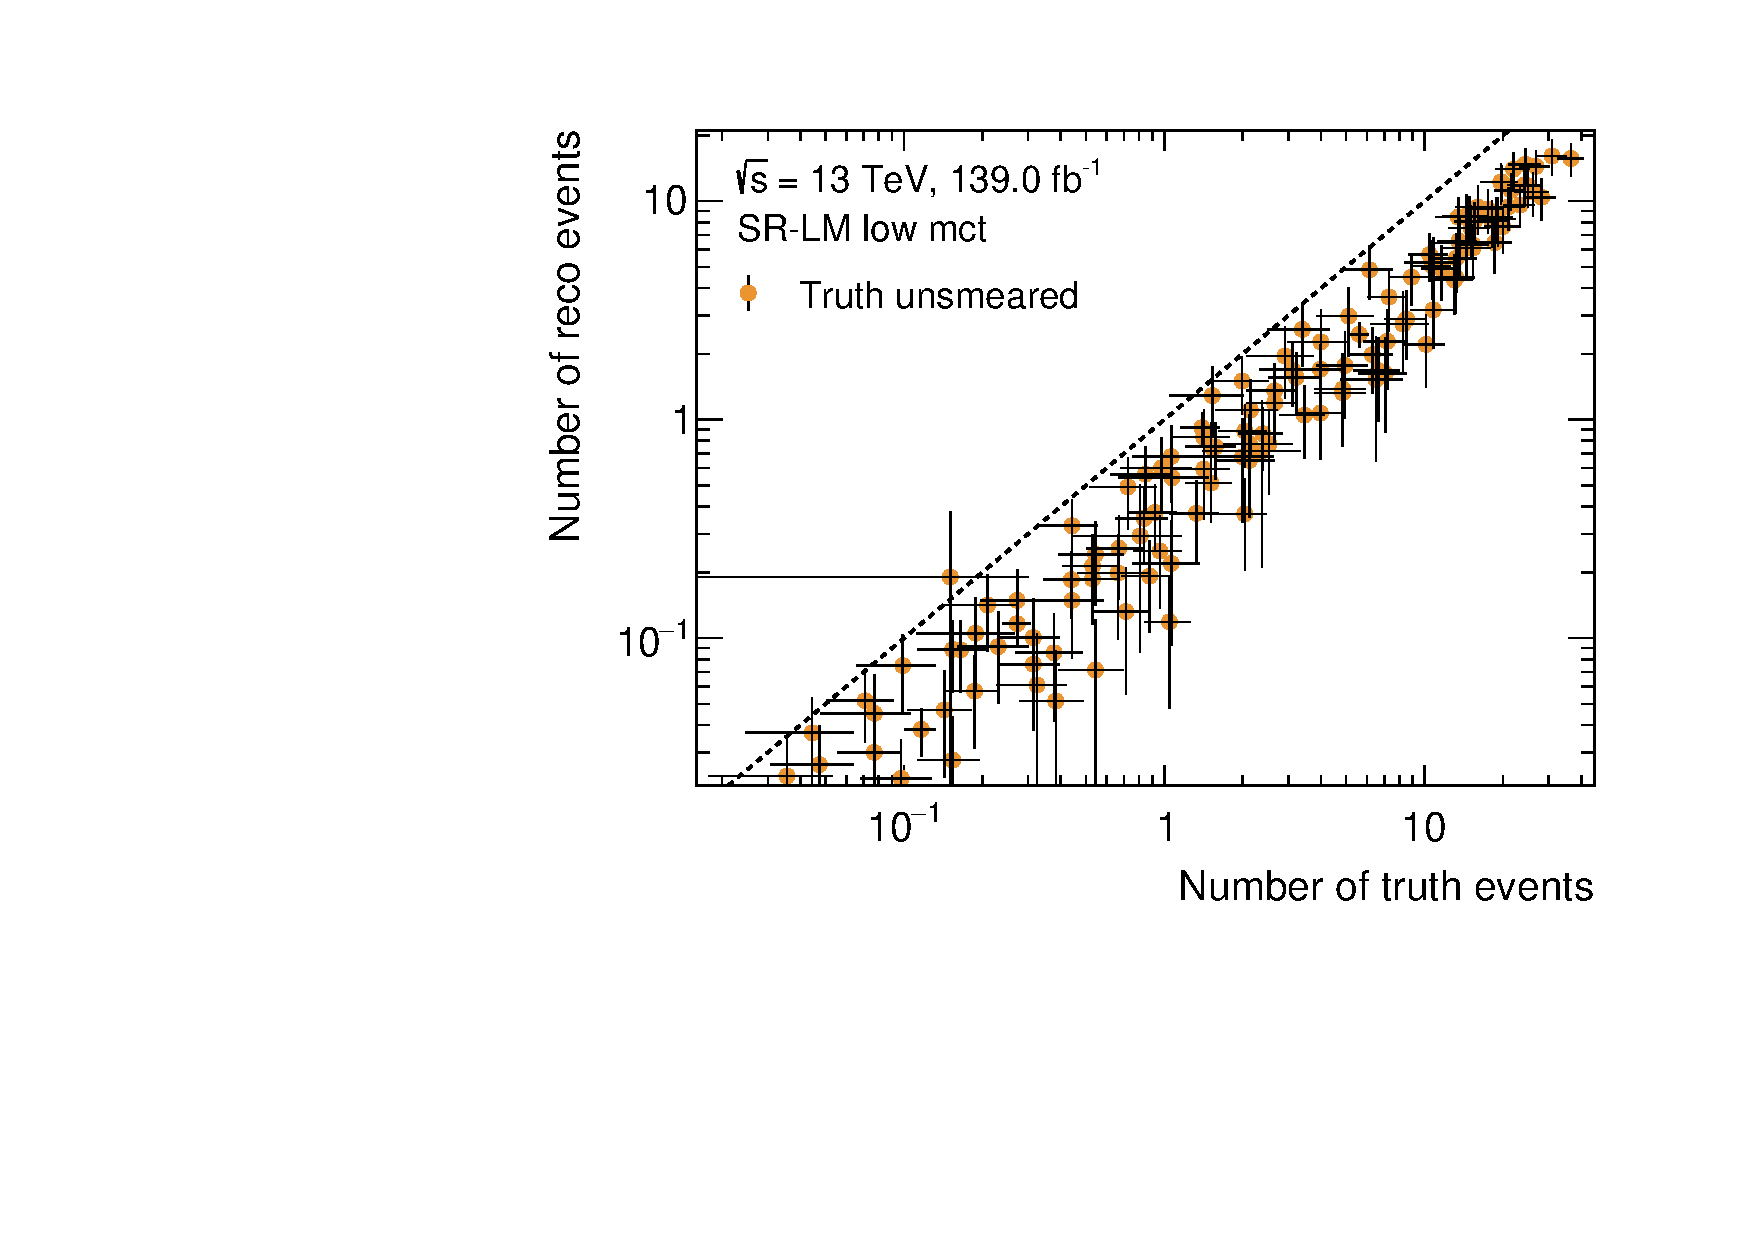
\includegraphics[width=\textwidth]{yields_SR-LM_low_mct_unsmeared}
	\end{subfigure}\hfill
	\begin{subfigure}[b]{0.49\linewidth}
		\centering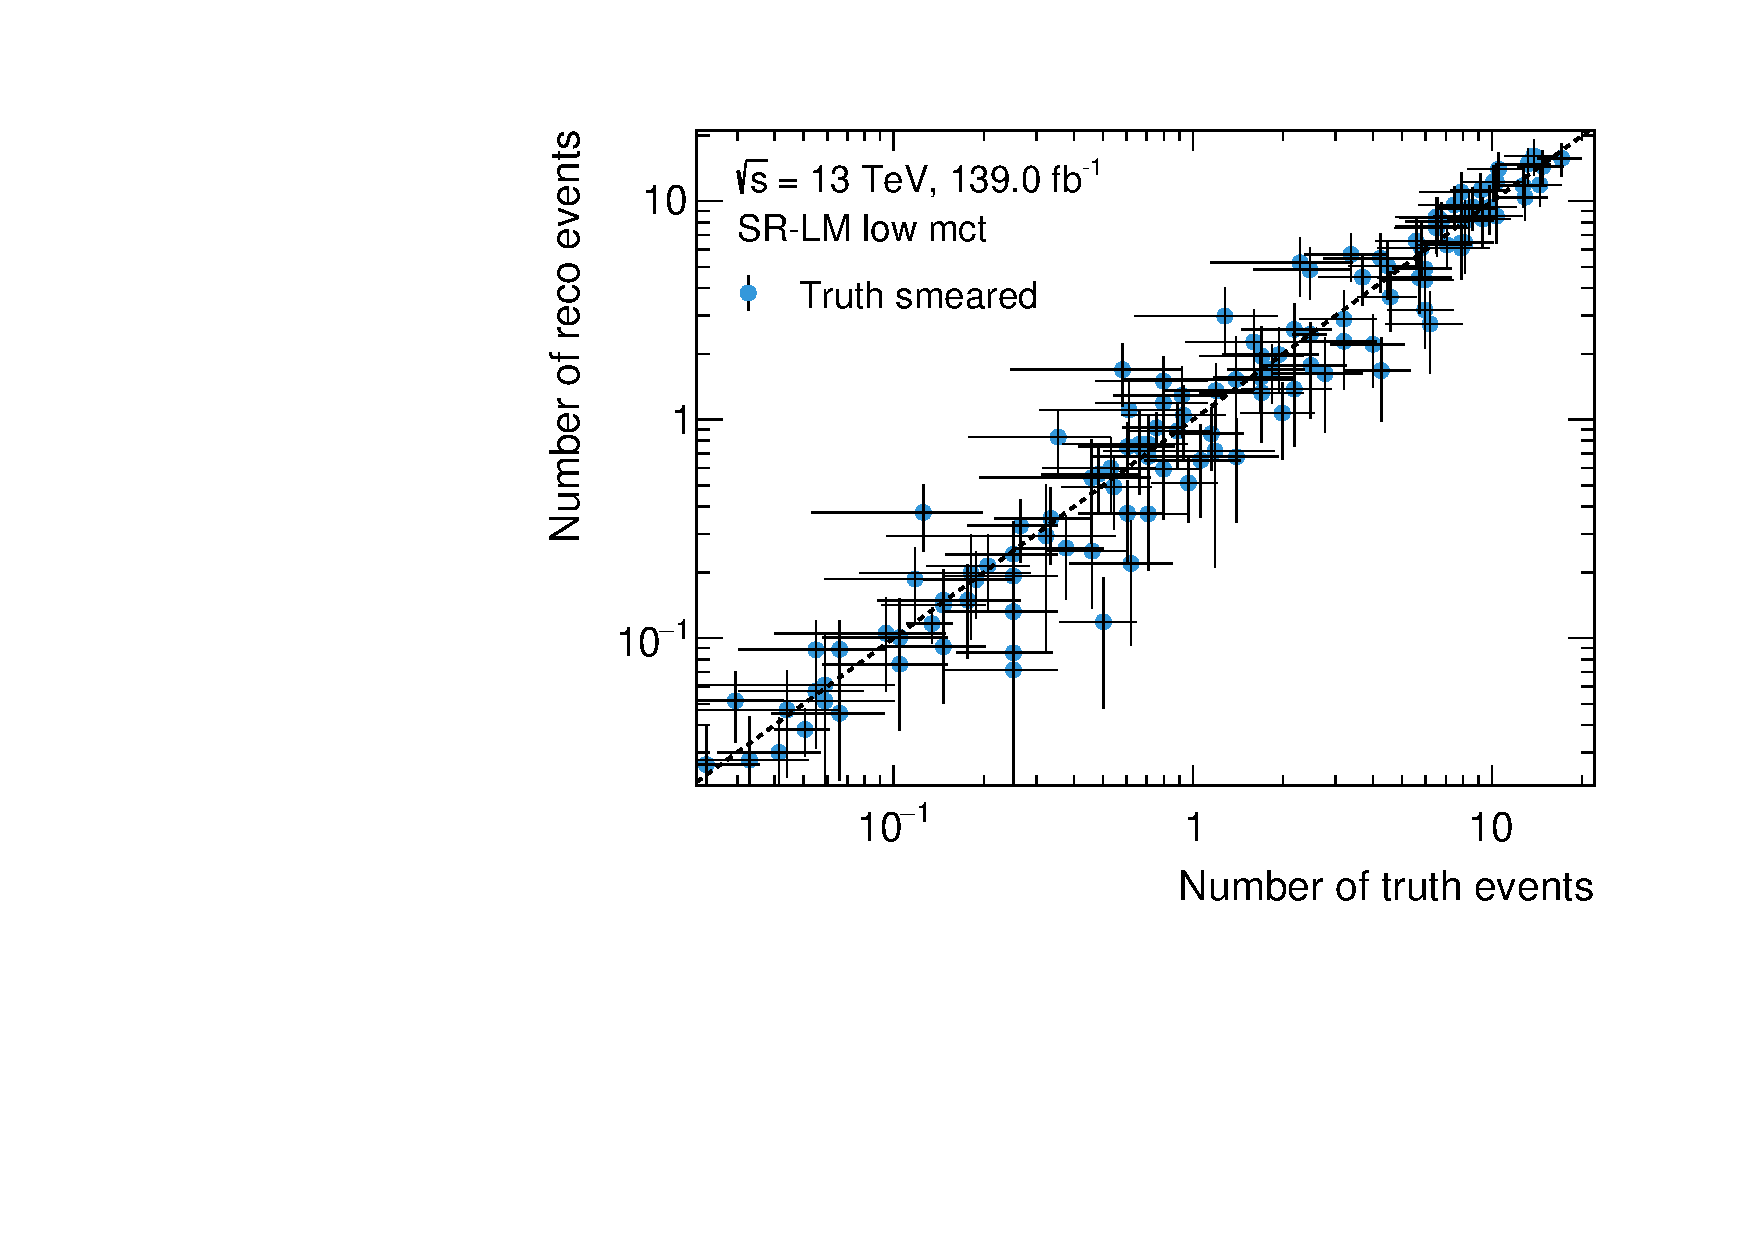
\includegraphics[width=\textwidth]{yields_SR-LM_low_mct_smeared}
	\end{subfigure}\hfill
	\begin{subfigure}[b]{0.49\linewidth}
		\centering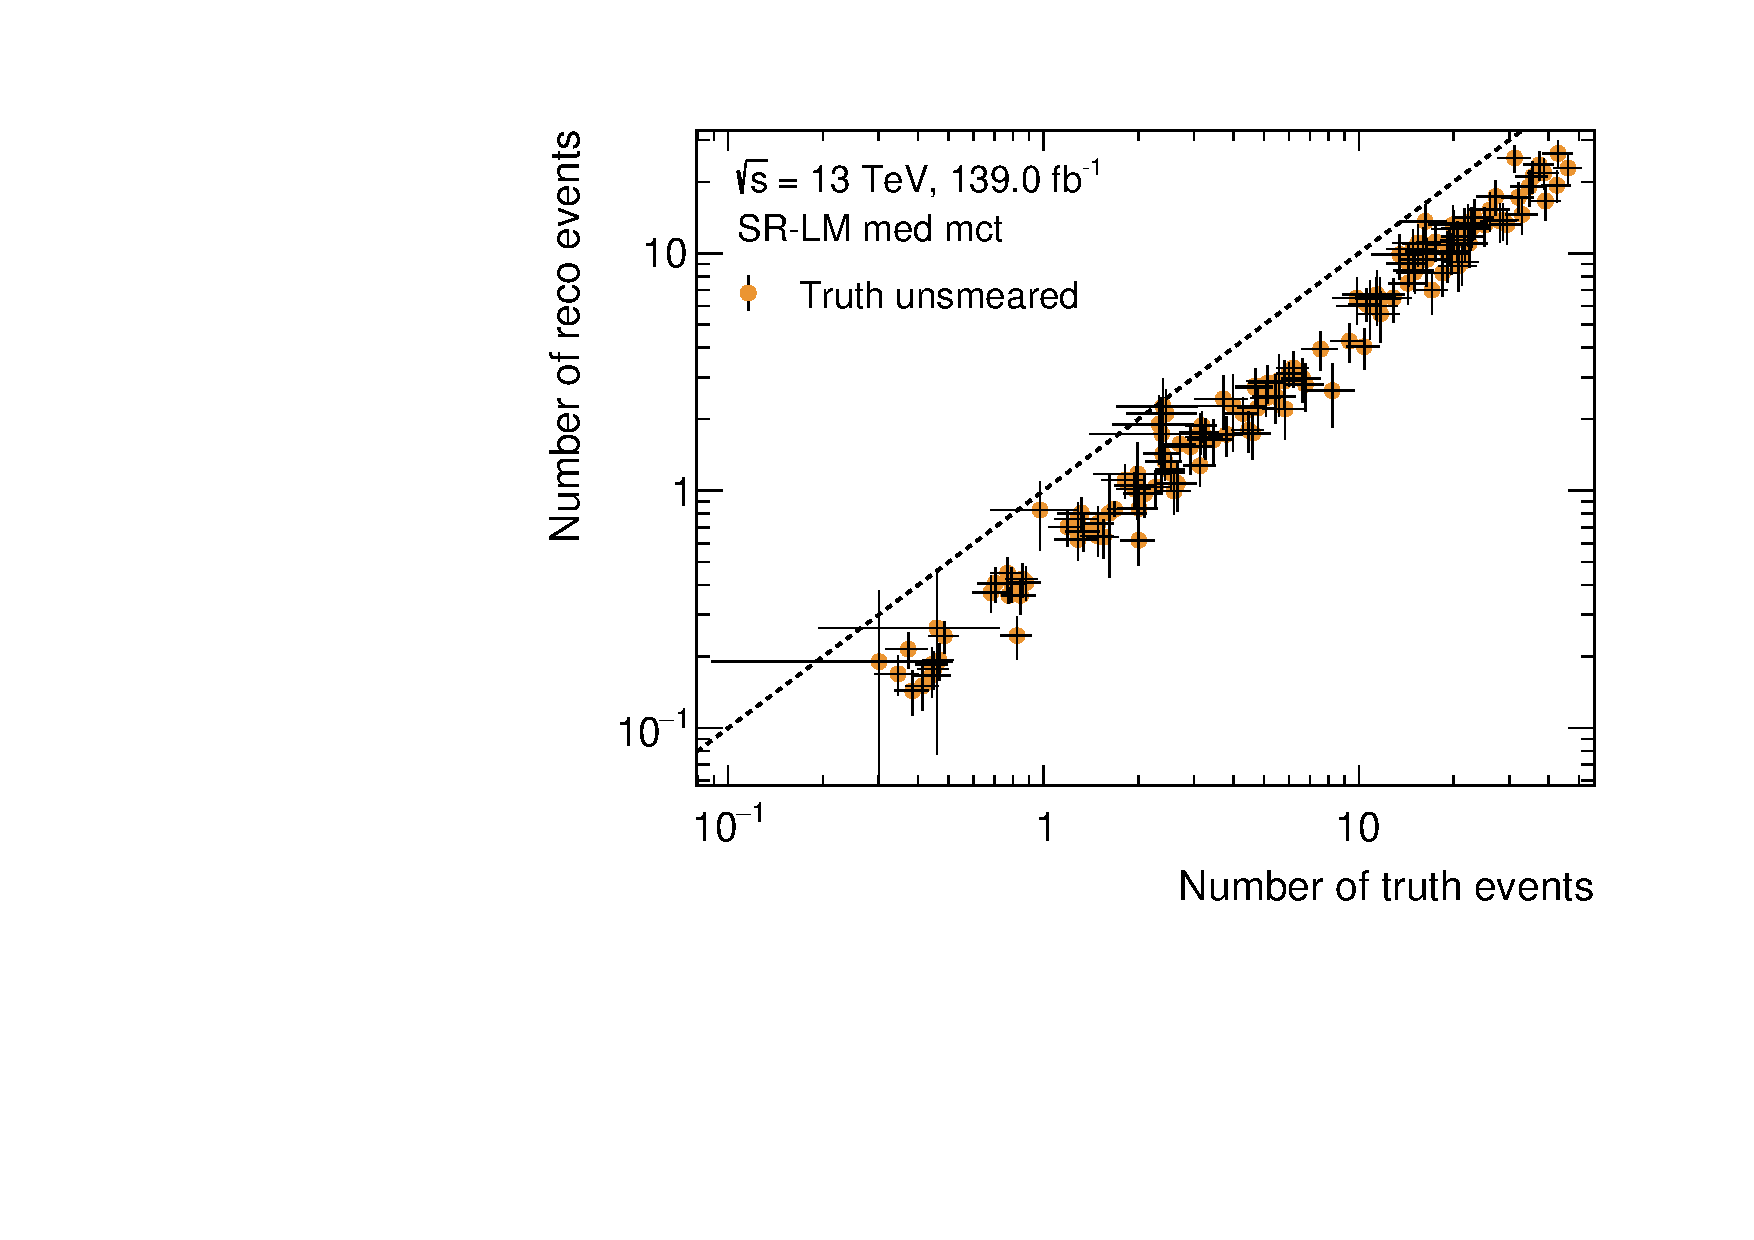
\includegraphics[width=\textwidth]{yields_SR-LM_med_mct_unsmeared}
	\end{subfigure}\hfill
	\begin{subfigure}[b]{0.49\linewidth}
		\centering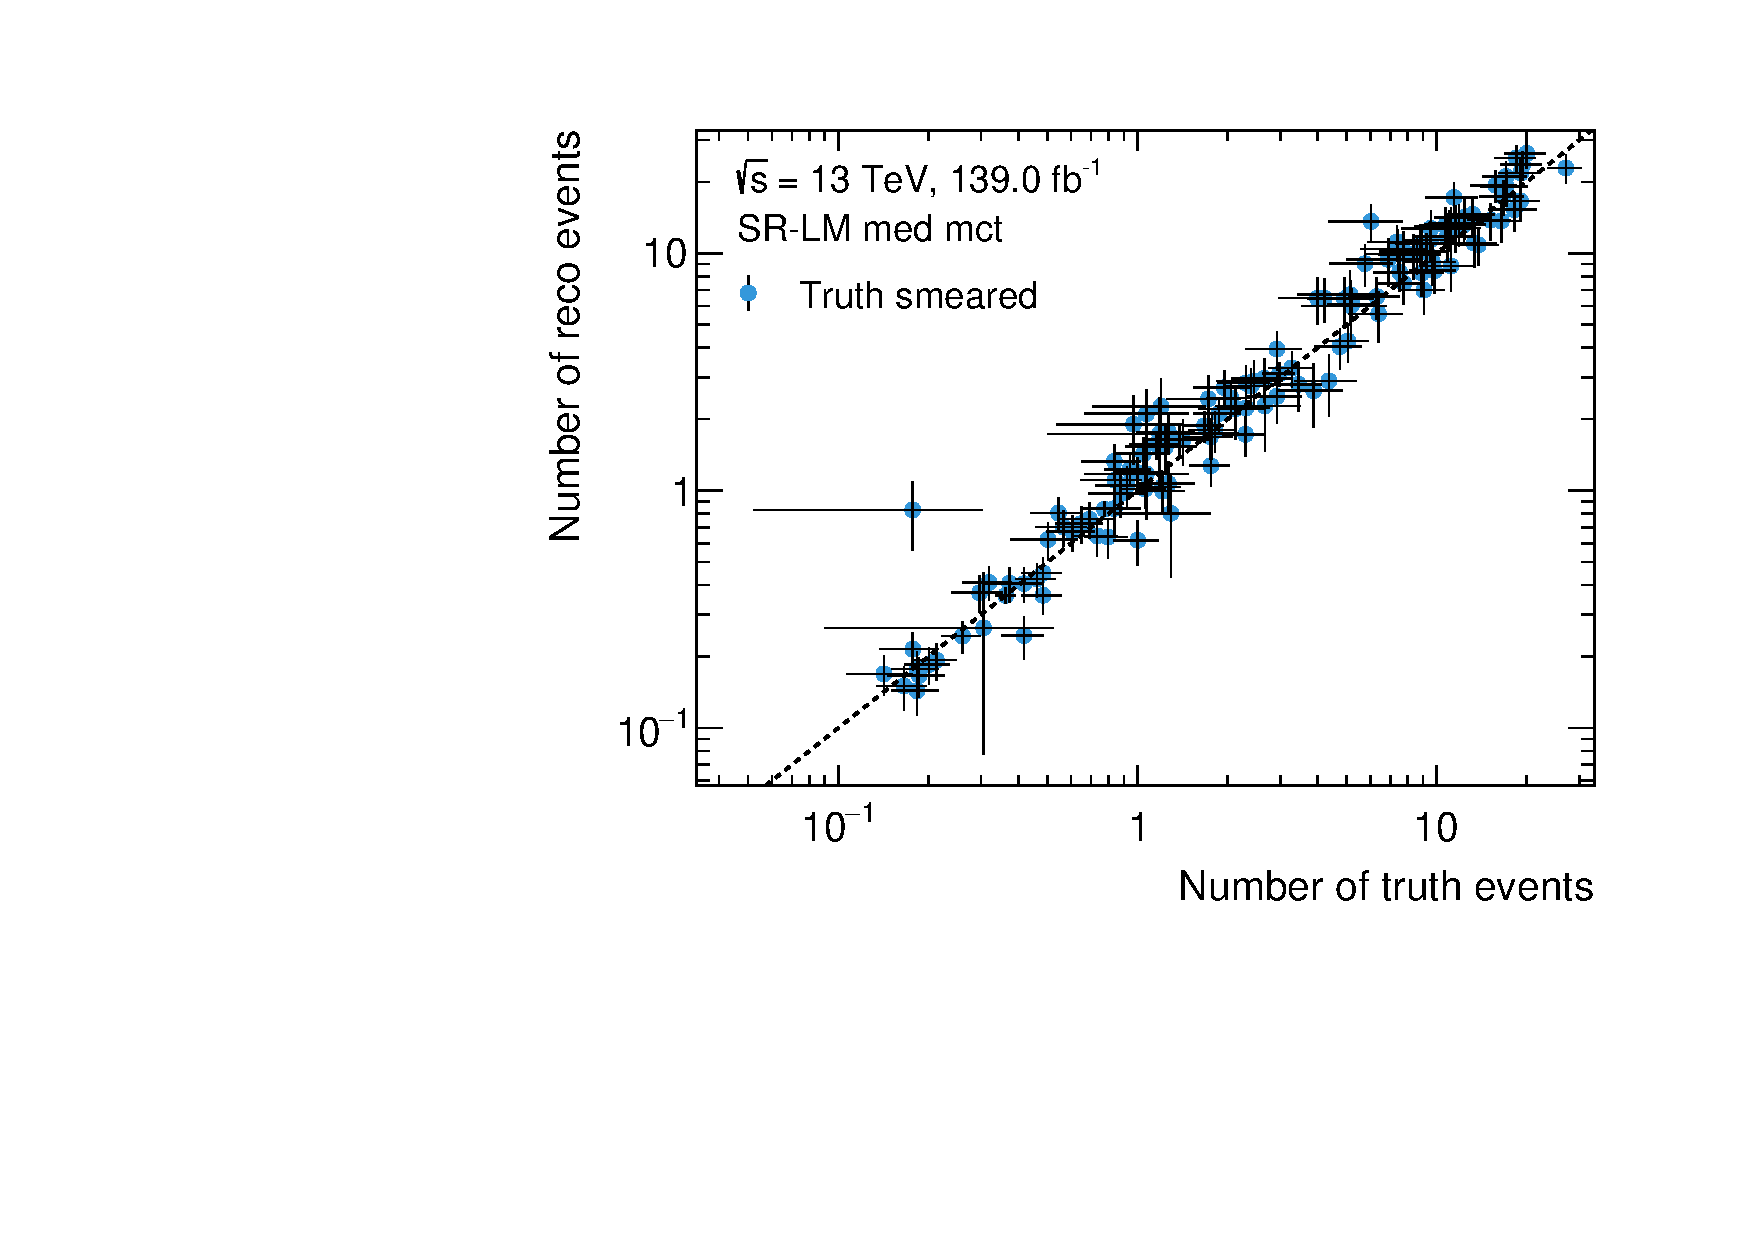
\includegraphics[width=\textwidth]{yields_SR-LM_med_mct_smeared}
	\end{subfigure}\hfill
	\begin{subfigure}[b]{0.49\linewidth}
		\centering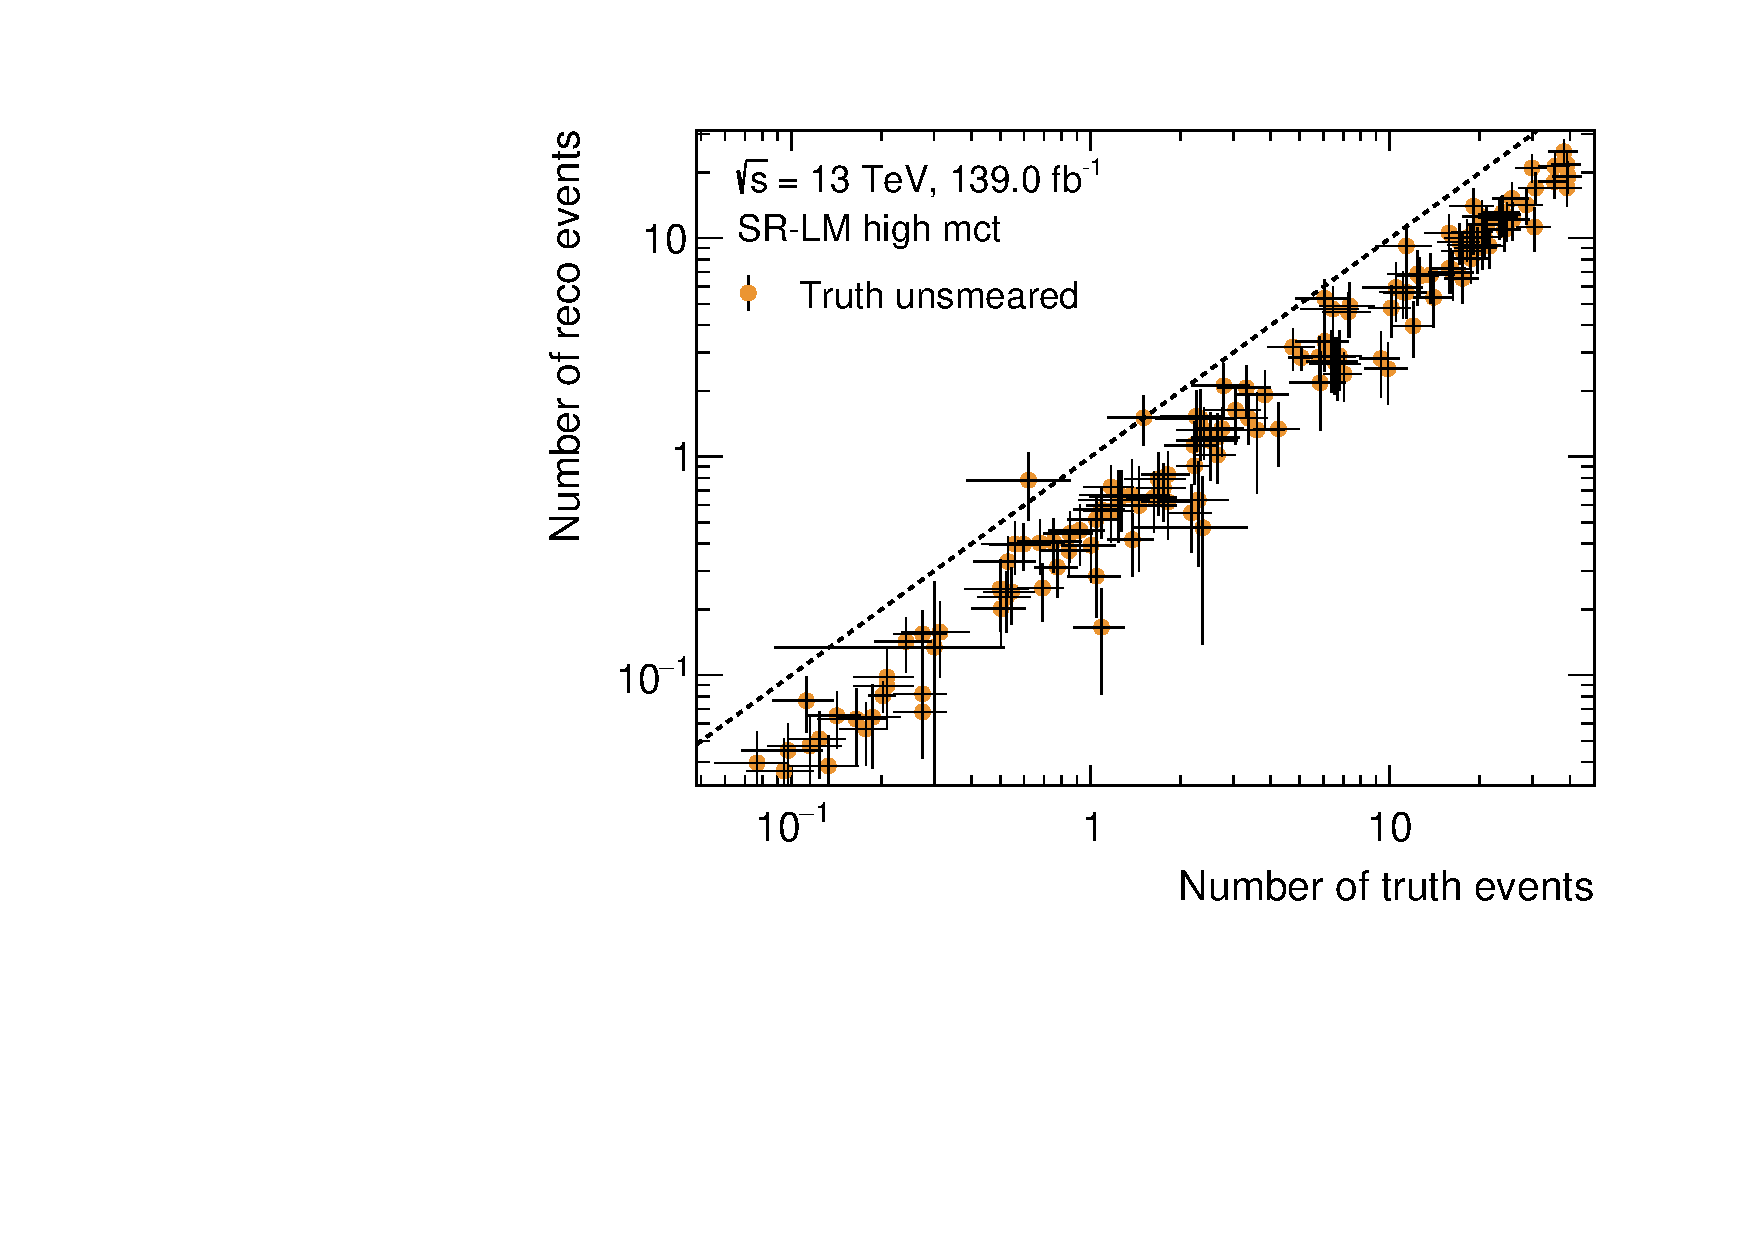
\includegraphics[width=\textwidth]{yields_SR-LM_high_mct_unsmeared}
	\end{subfigure}\hfill
	\begin{subfigure}[b]{0.49\linewidth}
		\centering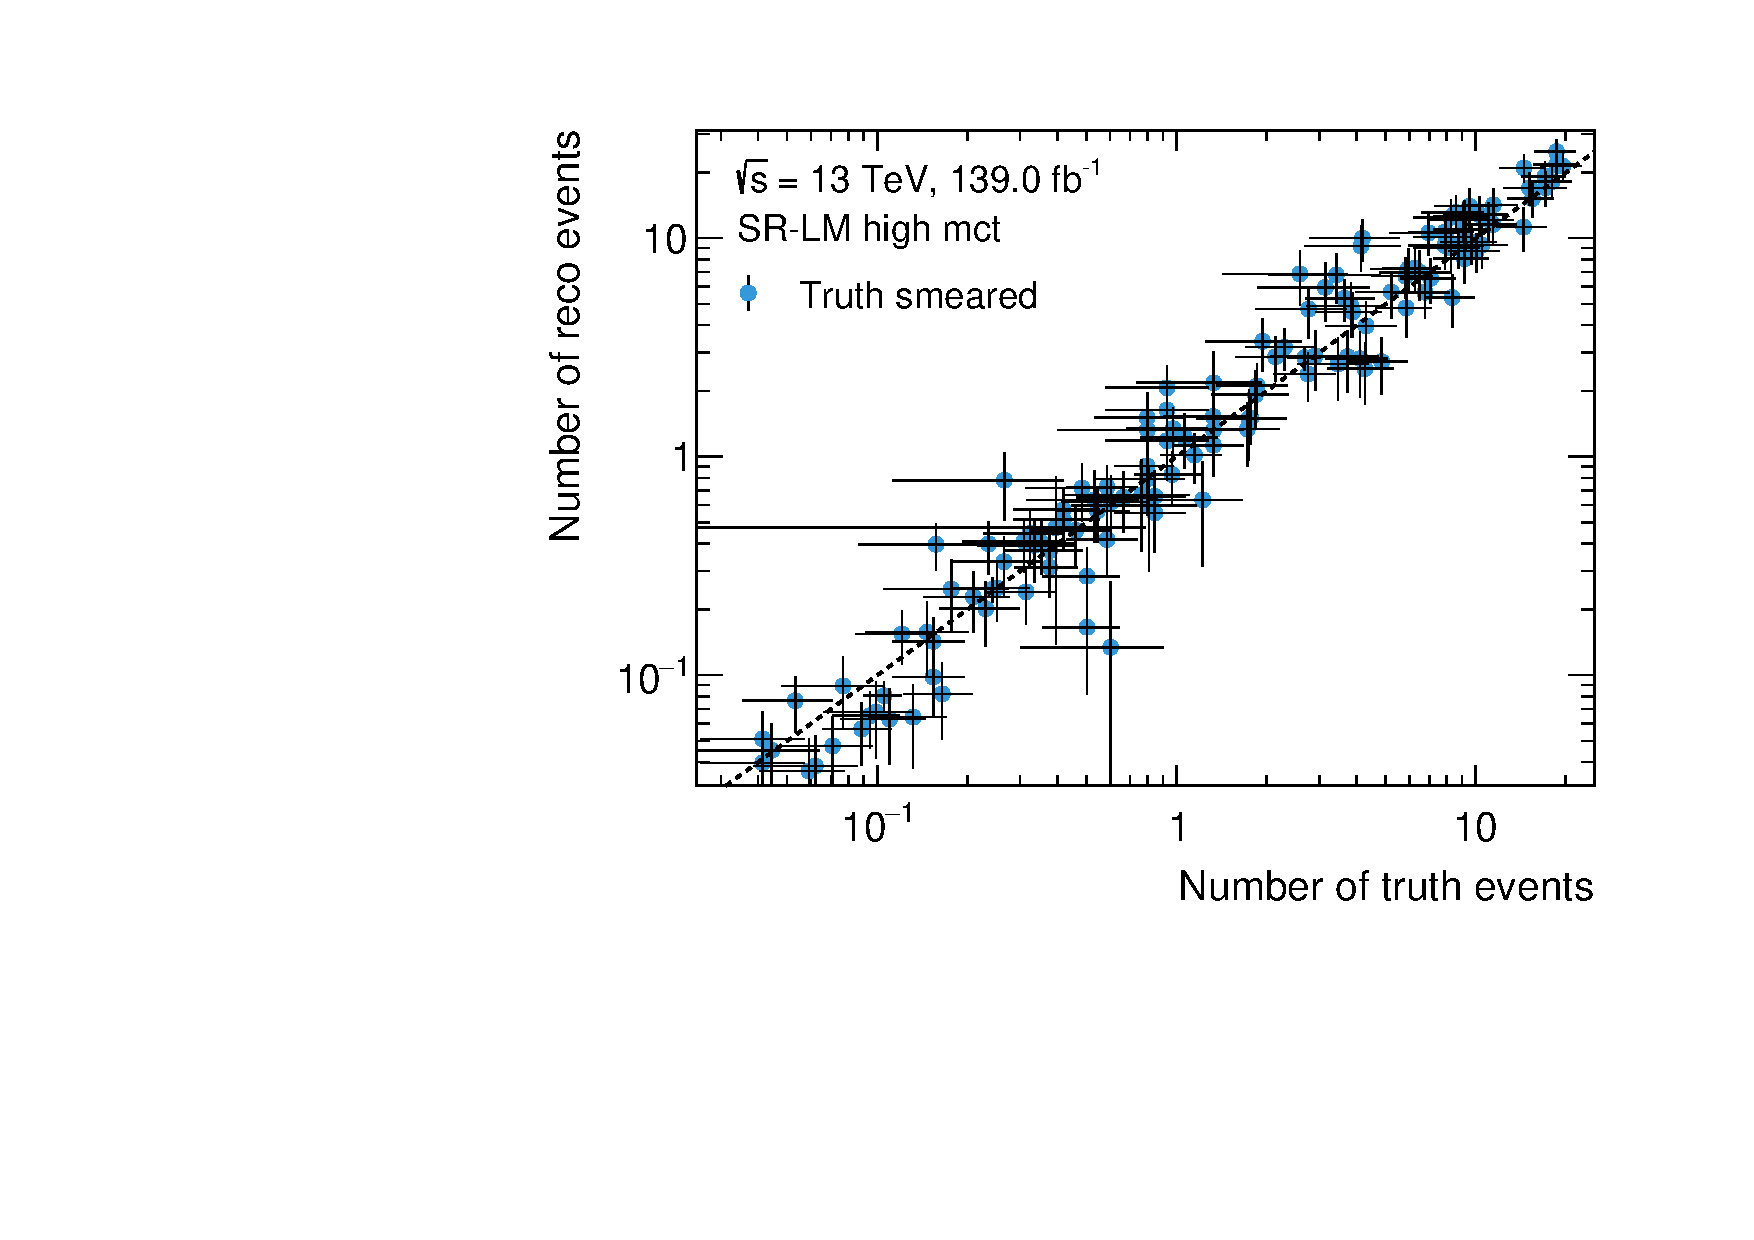
\includegraphics[width=\textwidth]{yields_SR-LM_high_mct_smeared}
	\end{subfigure}
	\caption{Comparison of the event rates at truth- and reconstruction-level before (left) and after (right) truth smearing in SR-LM. From top to bottom, the low, medium and high $\mct$ bins are shown. Every single point in the scatter plots represents a single signal model considered in the original 1-lepton analysis. Uncertainties include only \gls{mc} statistical uncertainties.}
	\label{fig:smearing_signal_regions_1}
\end{figure}

\begin{figure}
	\centering
	\begin{subfigure}[b]{0.49\linewidth}
		\centering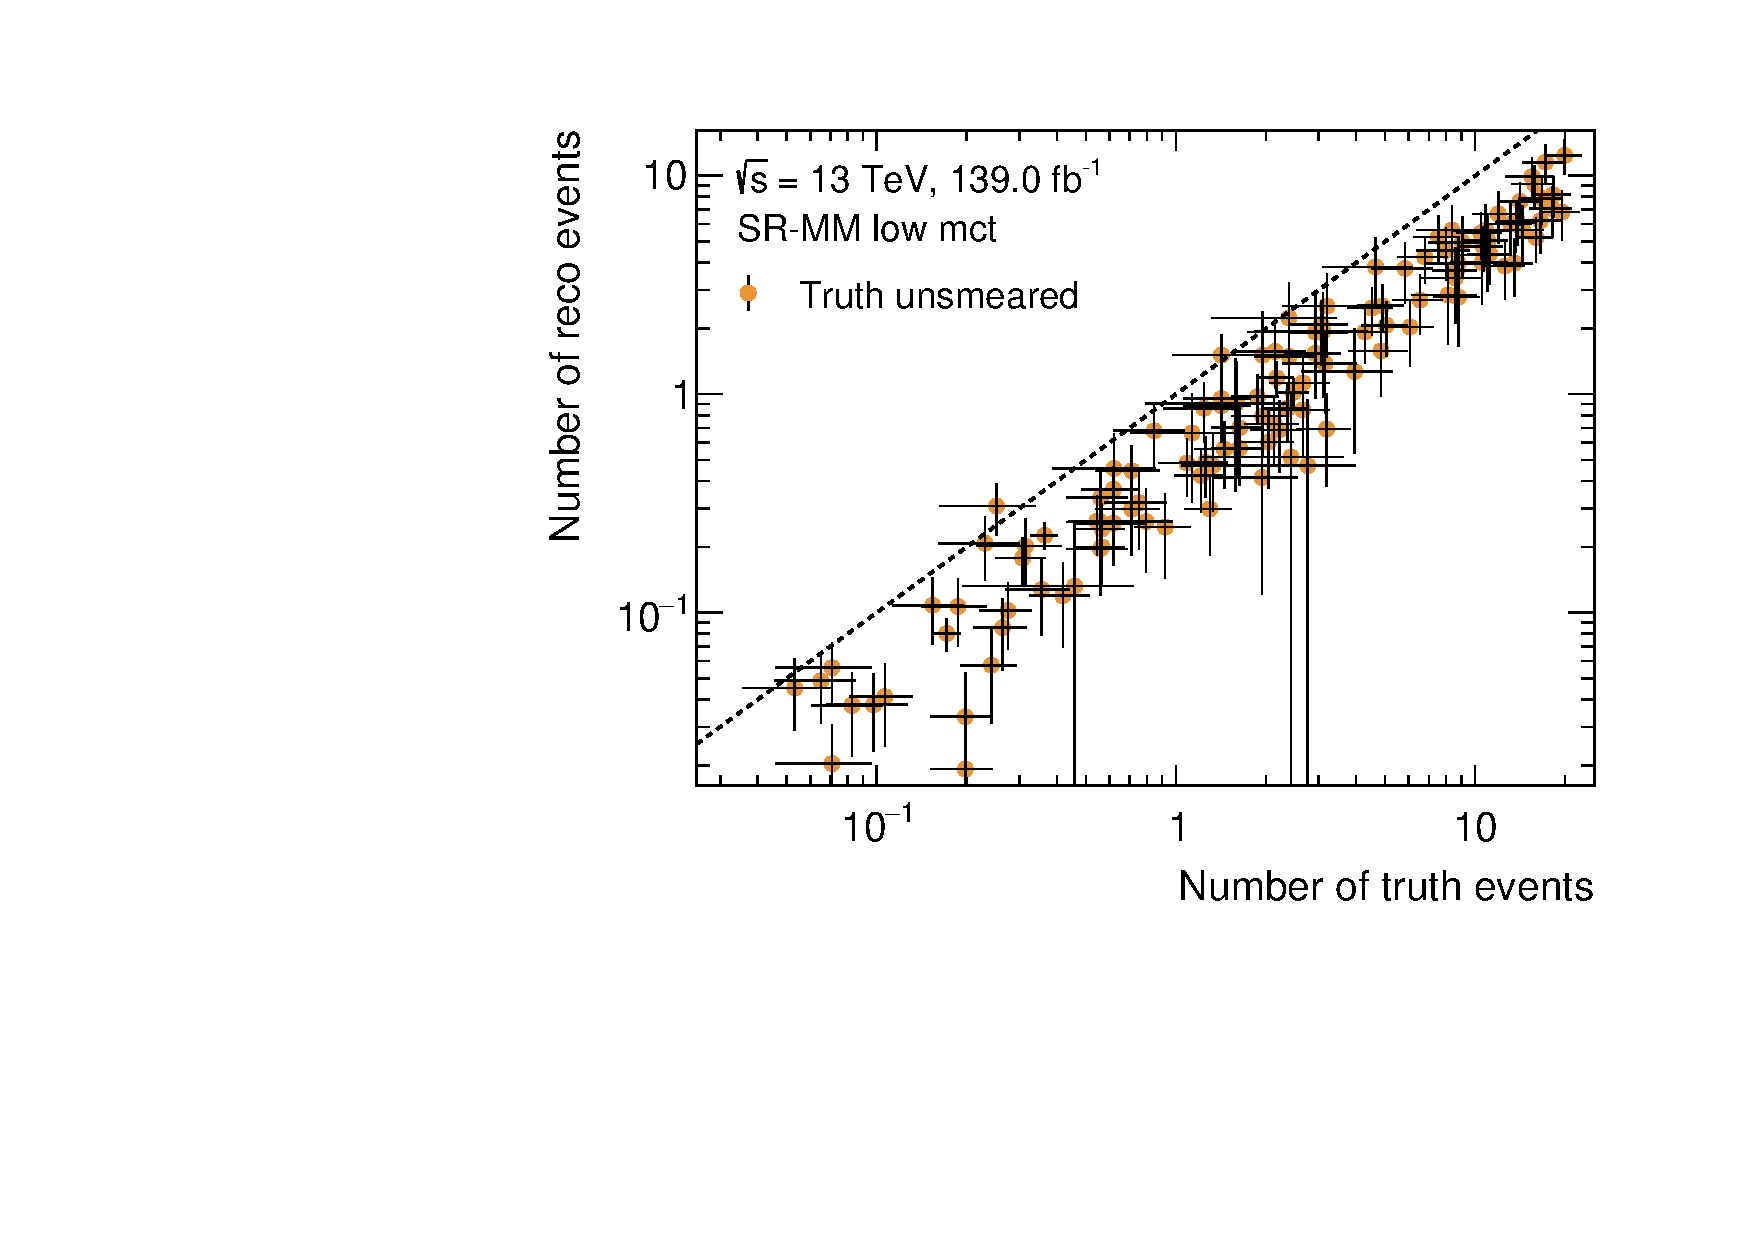
\includegraphics[width=\textwidth]{yields_SR-MM_low_mct_unsmeared}
	\end{subfigure}\hfill
	\begin{subfigure}[b]{0.49\linewidth}
		\centering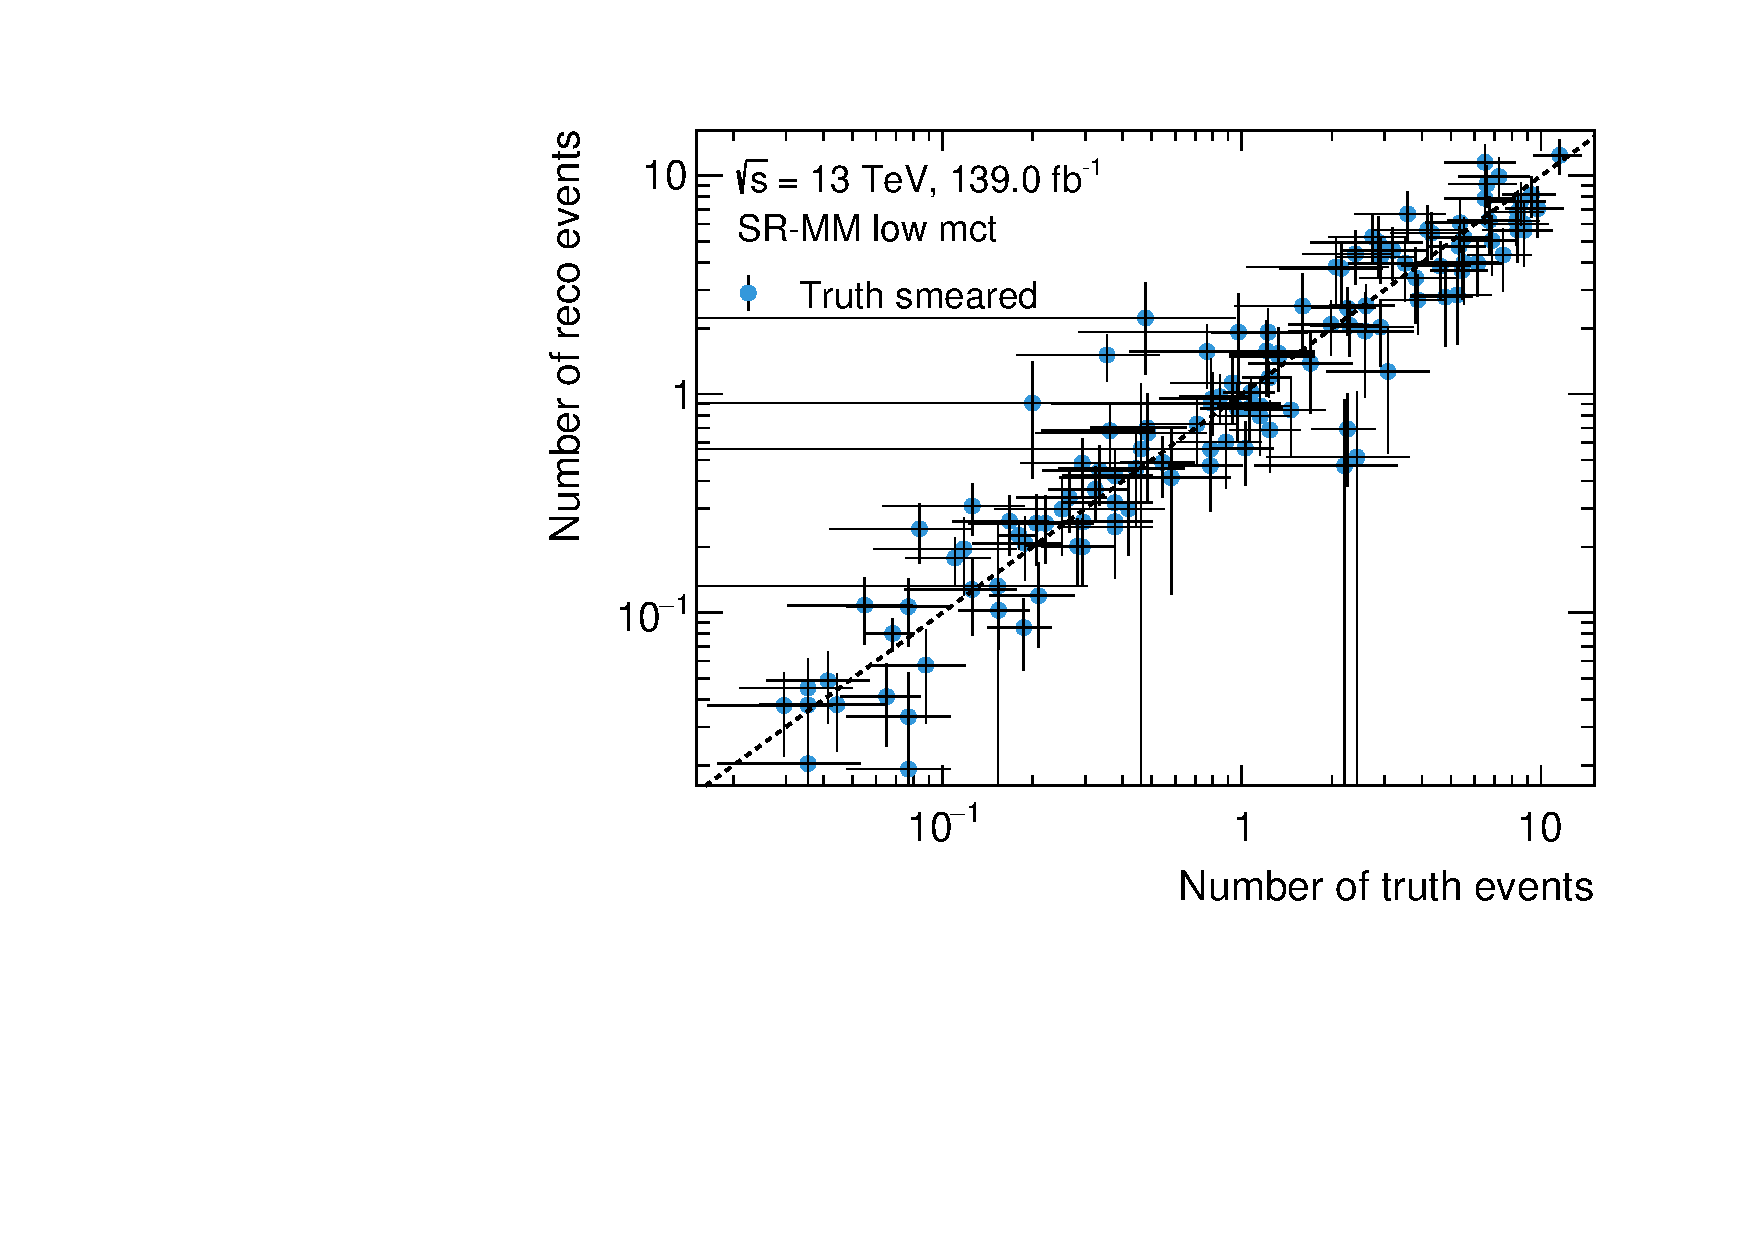
\includegraphics[width=\textwidth]{yields_SR-MM_low_mct_smeared}
	\end{subfigure}\hfill
	\begin{subfigure}[b]{0.49\linewidth}
		\centering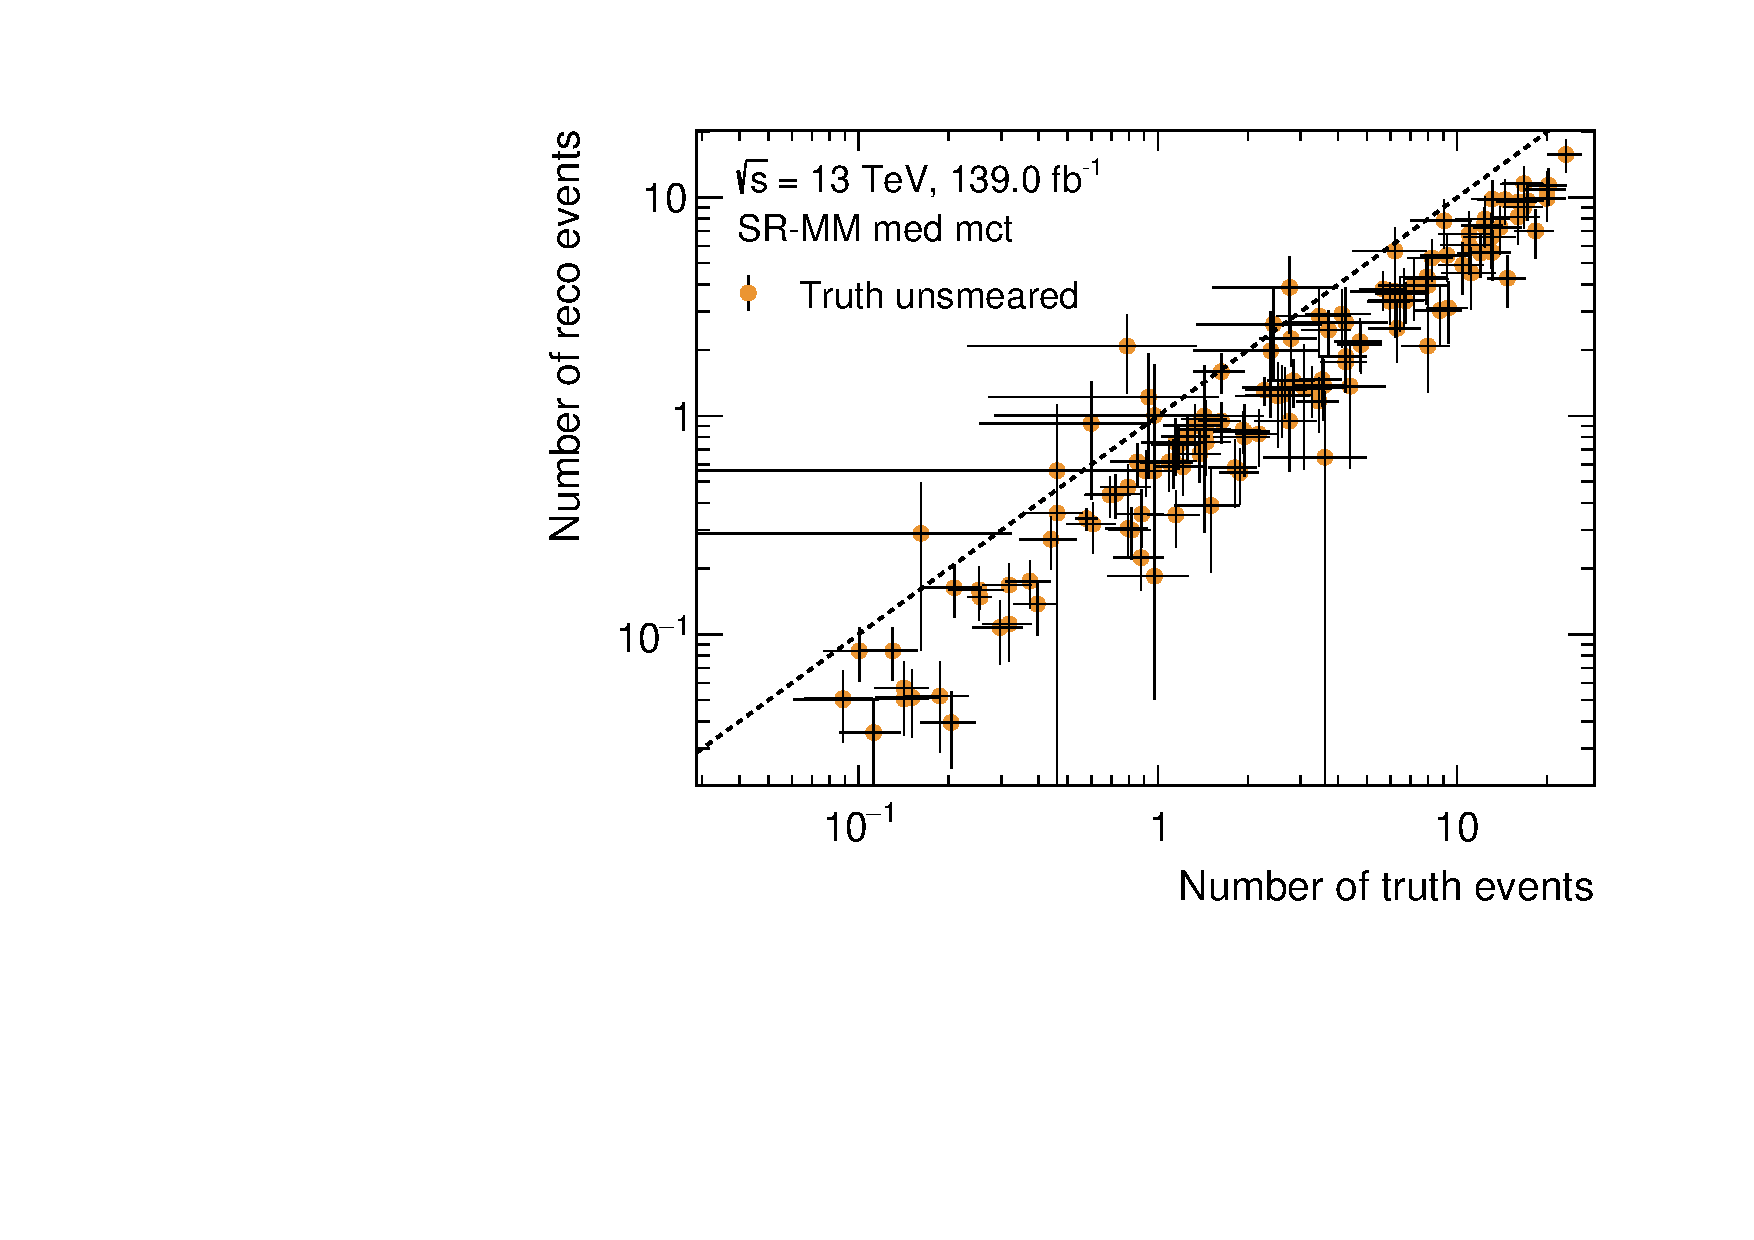
\includegraphics[width=\textwidth]{yields_SR-MM_med_mct_unsmeared}
	\end{subfigure}\hfill
	\begin{subfigure}[b]{0.49\linewidth}
		\centering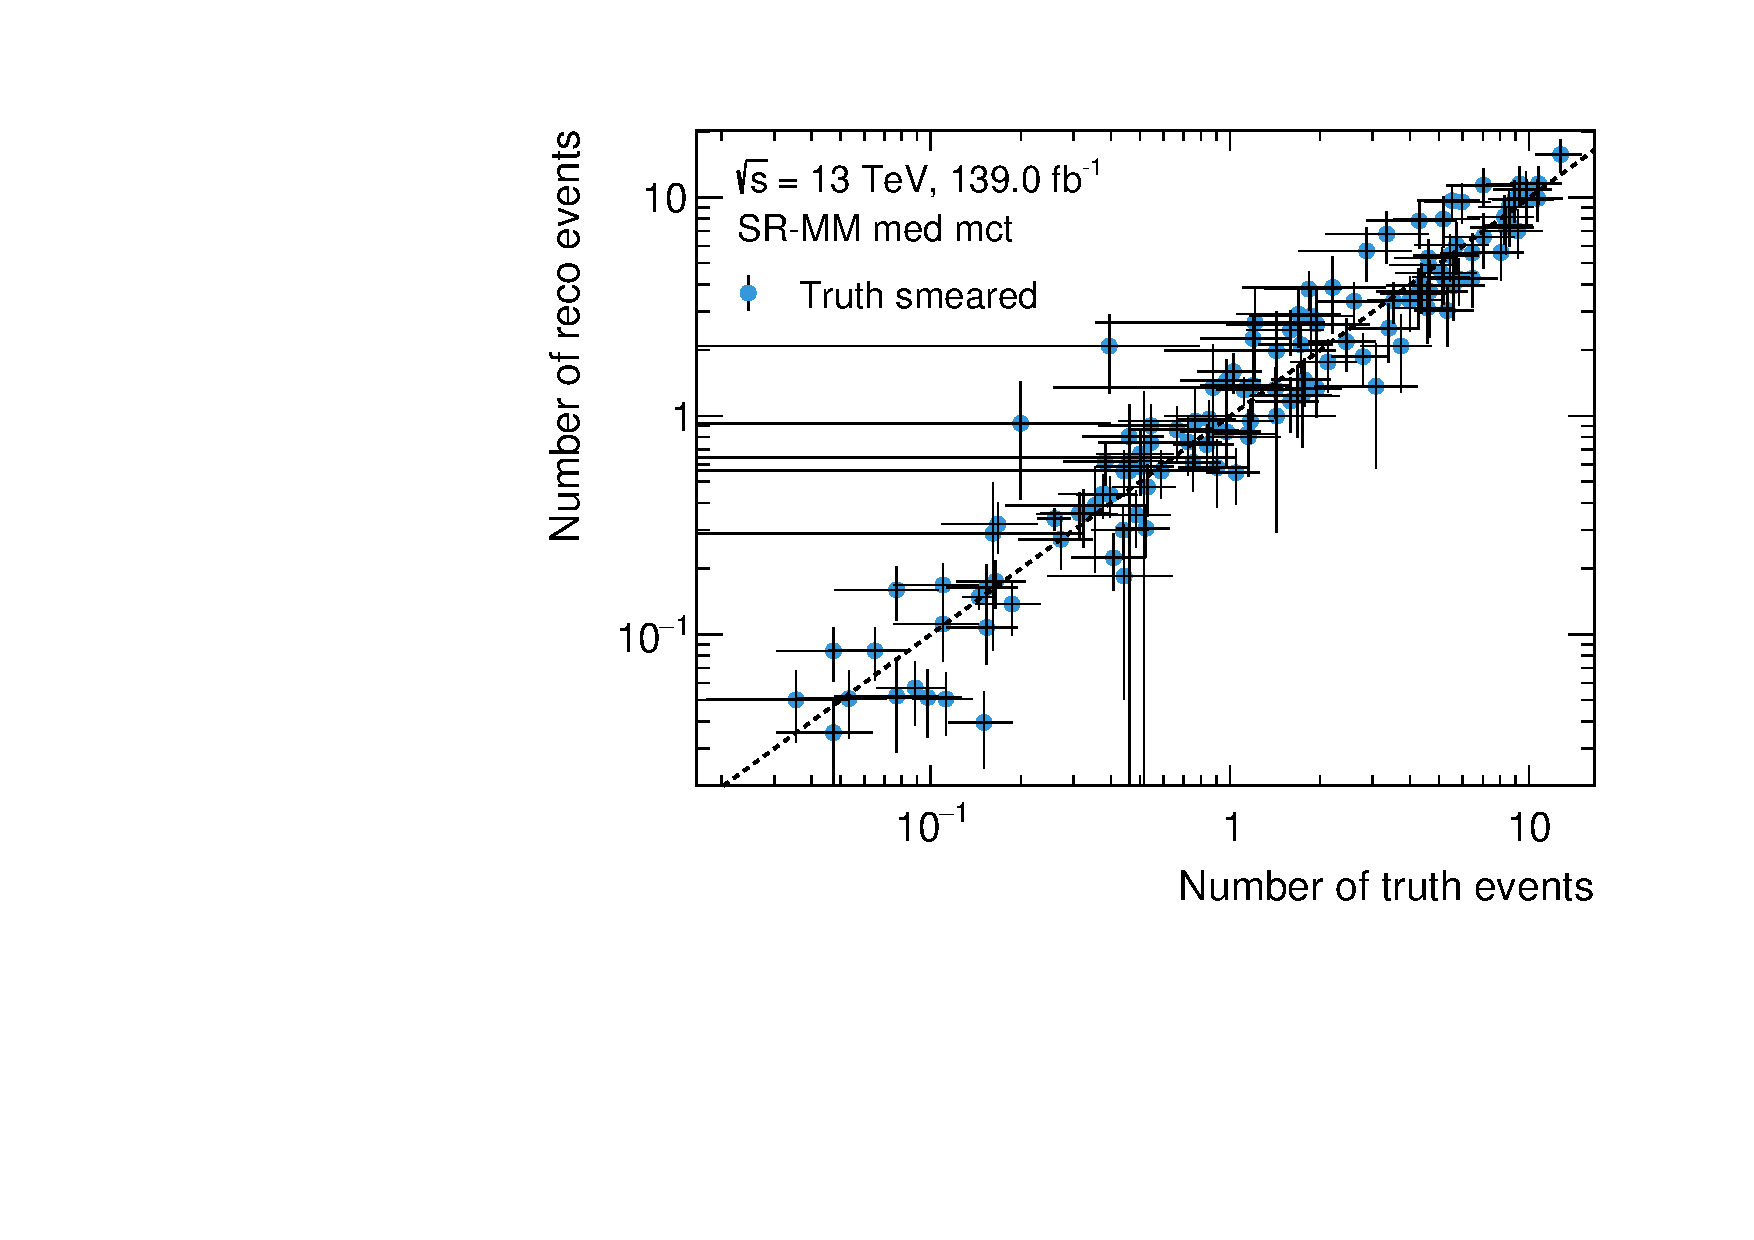
\includegraphics[width=\textwidth]{yields_SR-MM_med_mct_smeared}
	\end{subfigure}\hfill
	\begin{subfigure}[b]{0.49\linewidth}
		\centering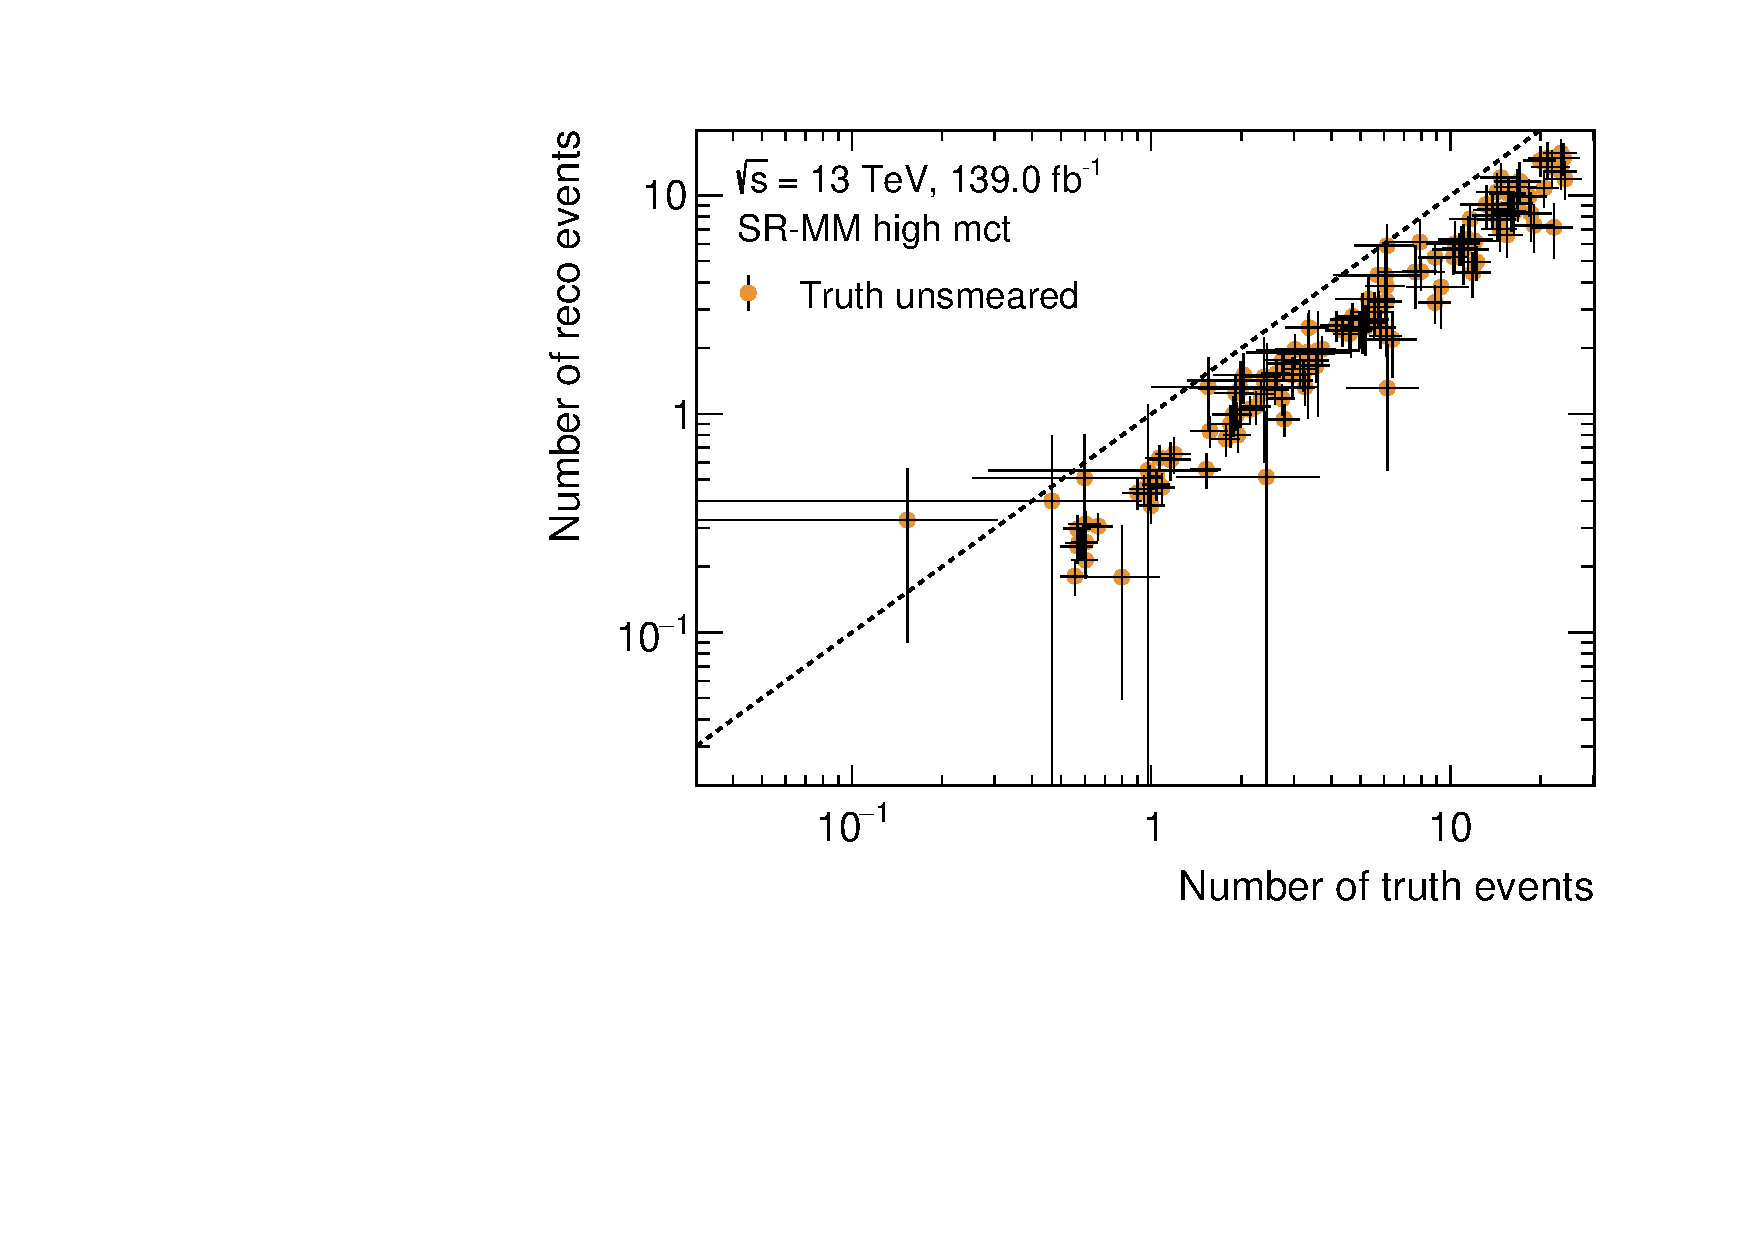
\includegraphics[width=\textwidth]{yields_SR-MM_high_mct_unsmeared}
	\end{subfigure}\hfill
	\begin{subfigure}[b]{0.49\linewidth}
		\centering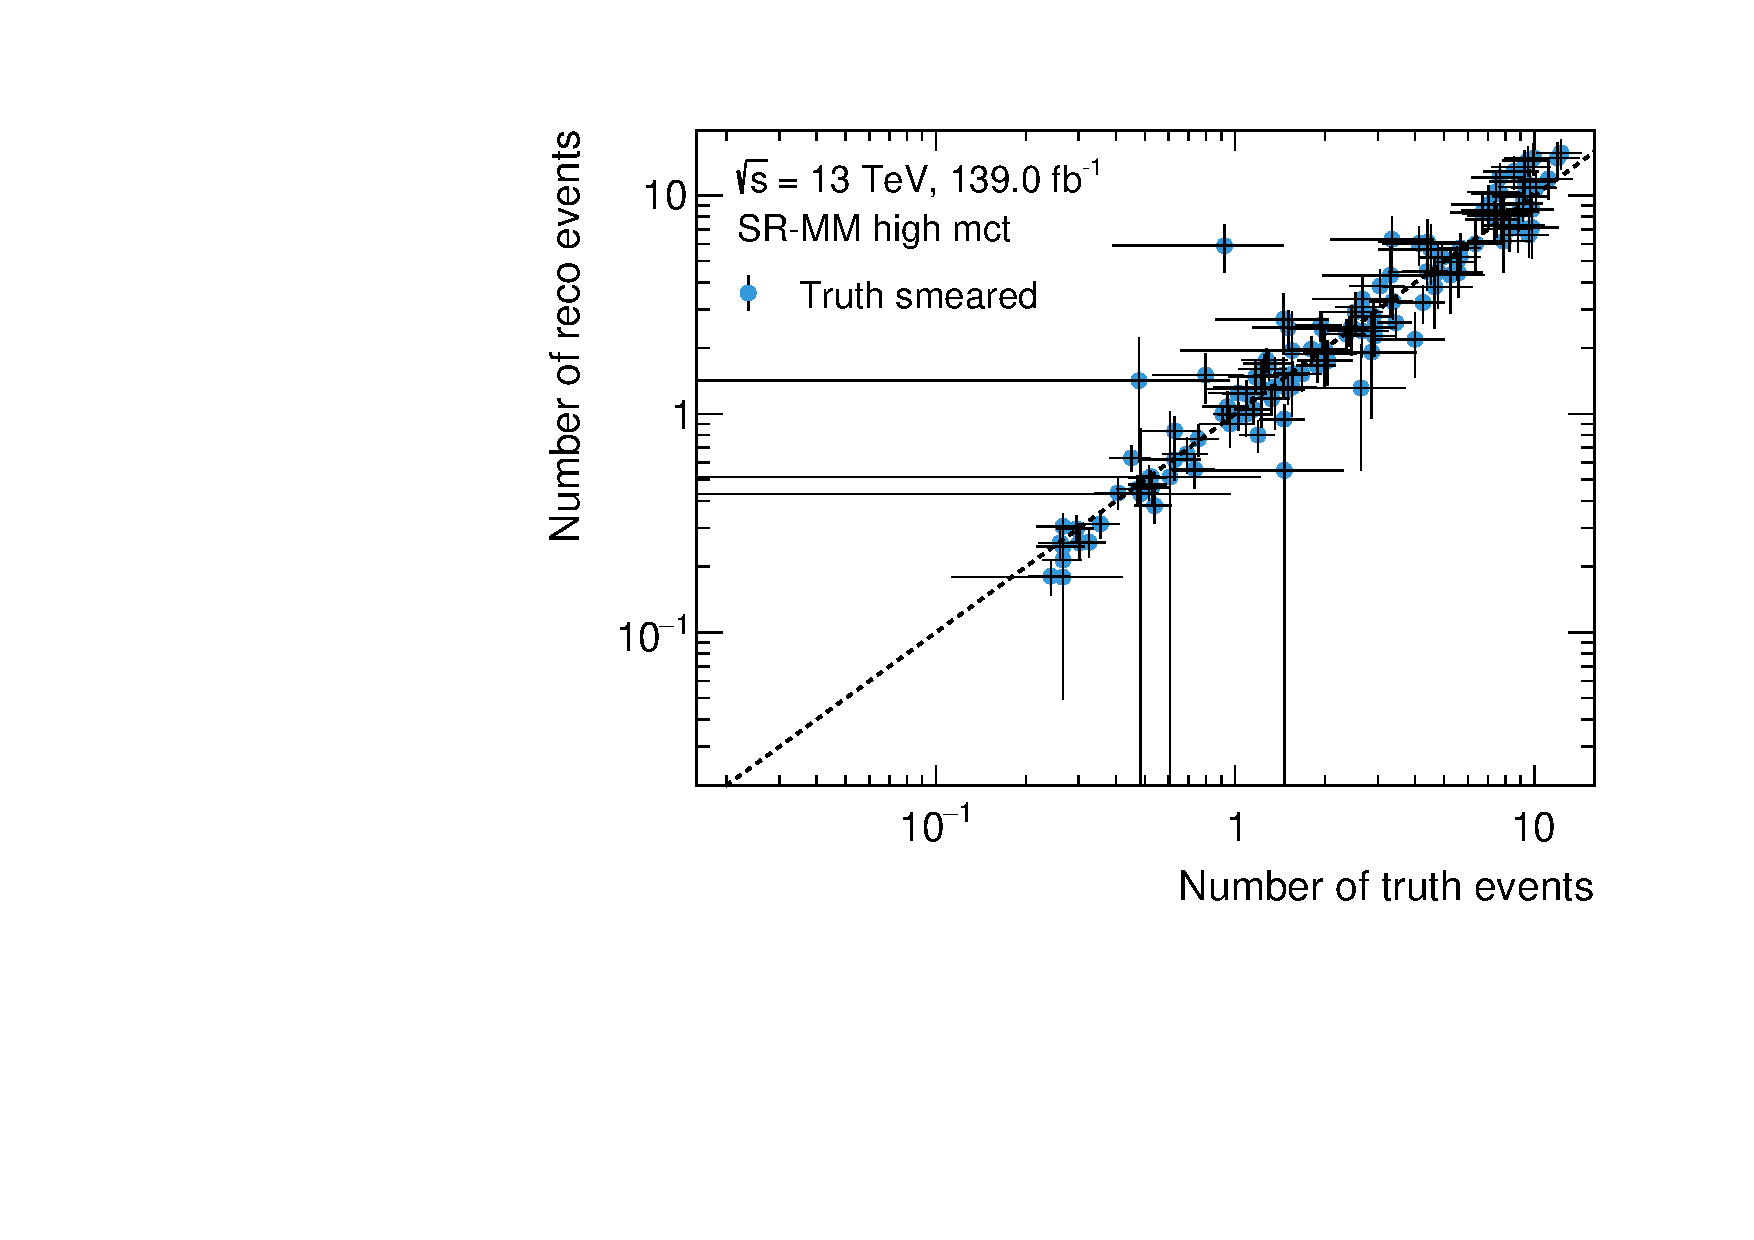
\includegraphics[width=\textwidth]{yields_SR-MM_high_mct_smeared}
	\end{subfigure}
	\caption{Comparison of the event rates at truth- and reconstruction-level before (left) and after (right) truth smearing in SR-MM. From top to bottom, the low, medium and high $\mct$ bins are shown. Every single point in the scatter plots represents a single signal model considered in the original 1-lepton analysis. Uncertainties include only \gls{mc} statistical uncertainties.}
	\label{fig:smearing_signal_regions_2}
\end{figure}

\begin{figure}
	\centering
	\begin{subfigure}[b]{0.49\linewidth}
		\centering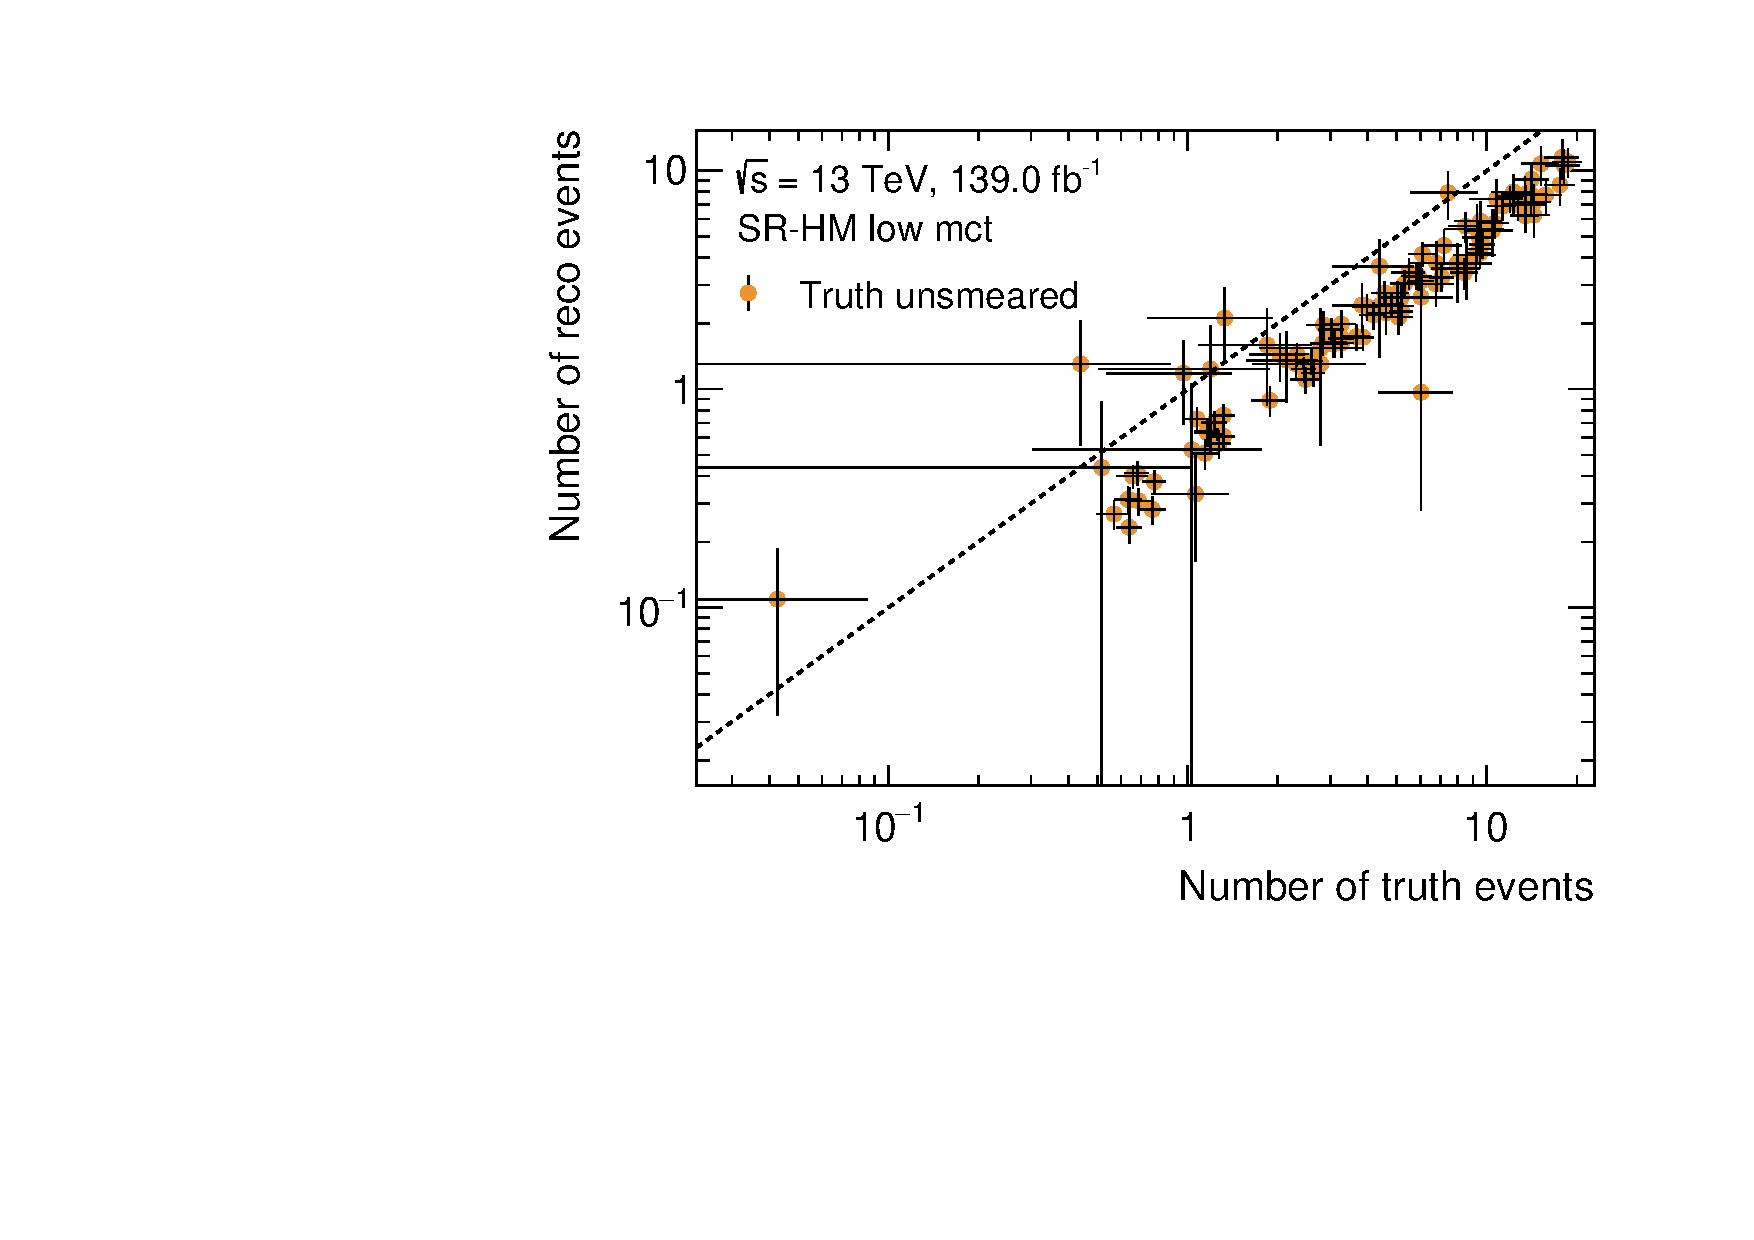
\includegraphics[width=\textwidth]{yields_SR-HM_low_mct_unsmeared}
	\end{subfigure}\hfill
	\begin{subfigure}[b]{0.49\linewidth}
		\centering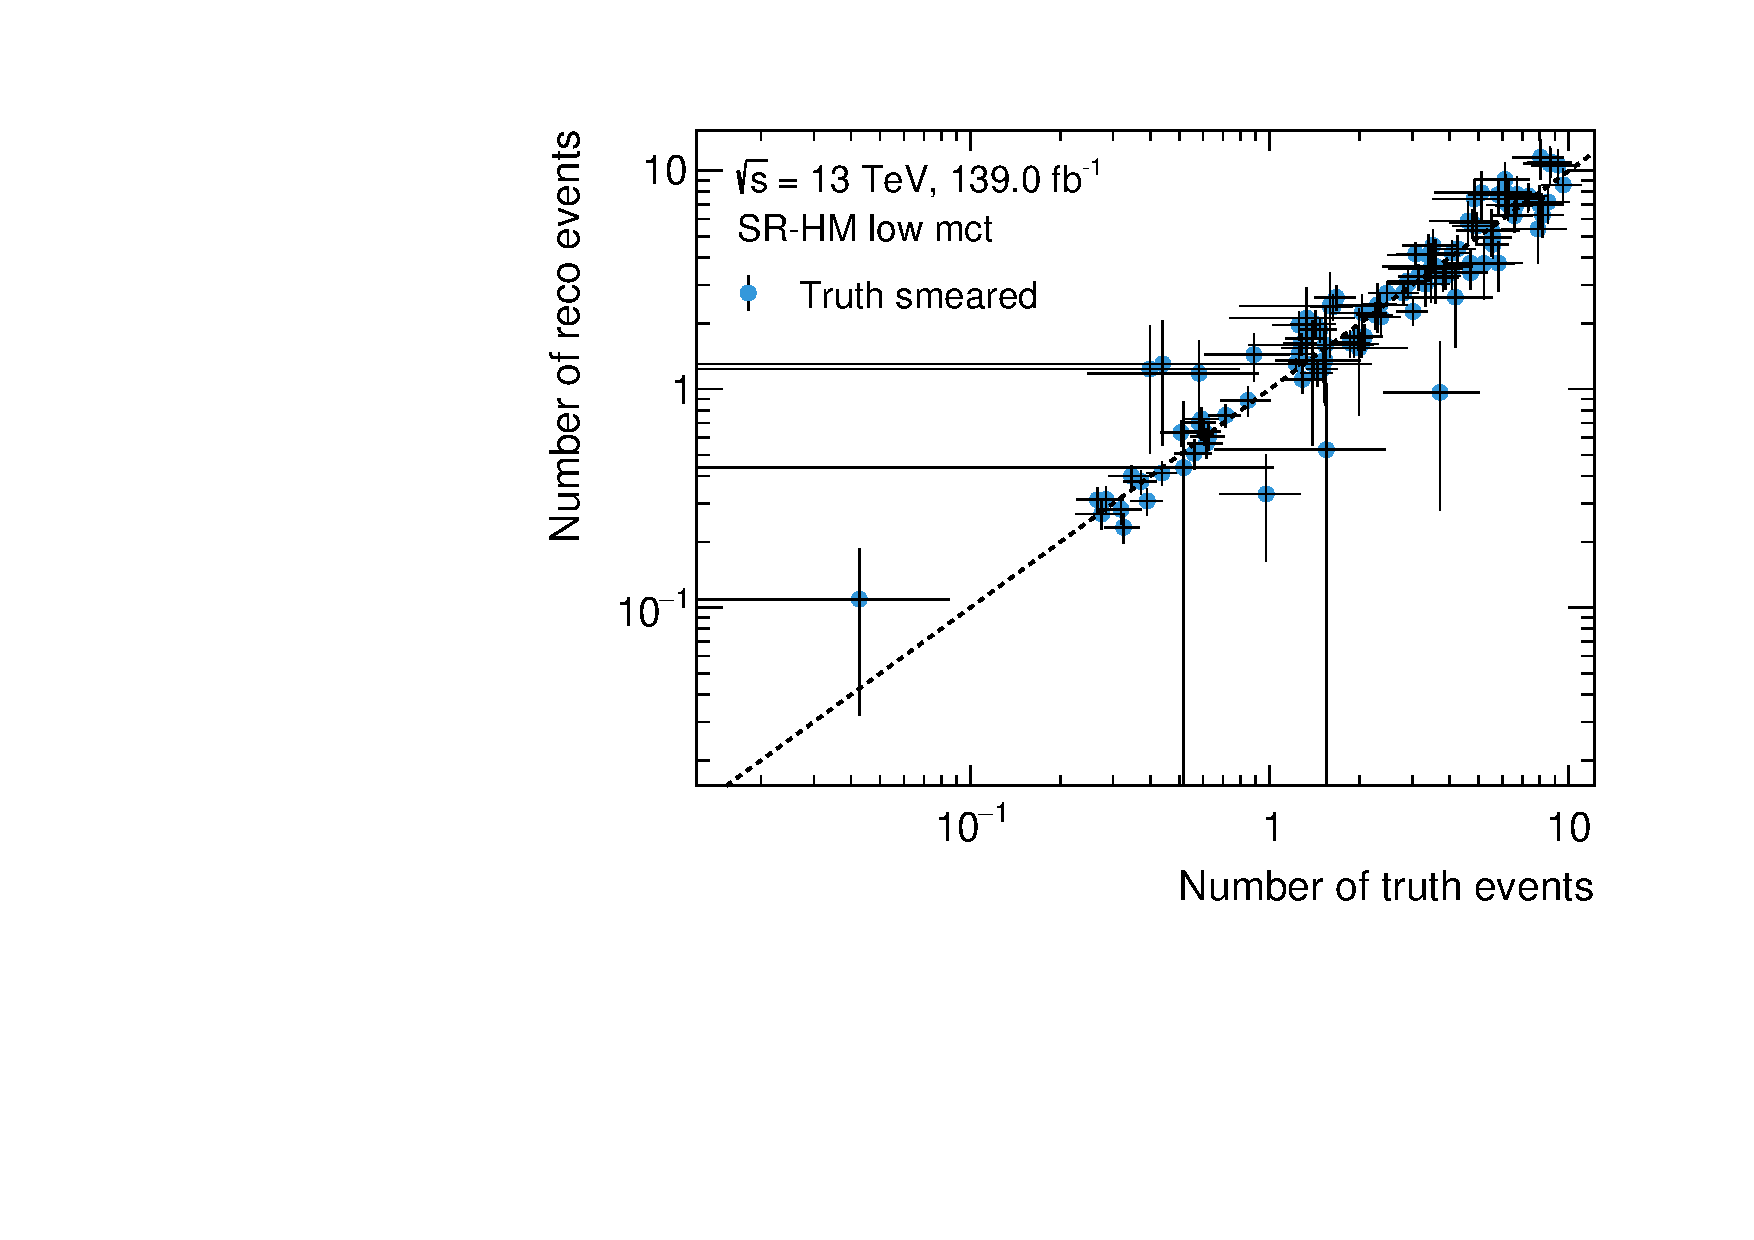
\includegraphics[width=\textwidth]{yields_SR-HM_low_mct_smeared}
	\end{subfigure}\hfill
	\begin{subfigure}[b]{0.49\linewidth}
		\centering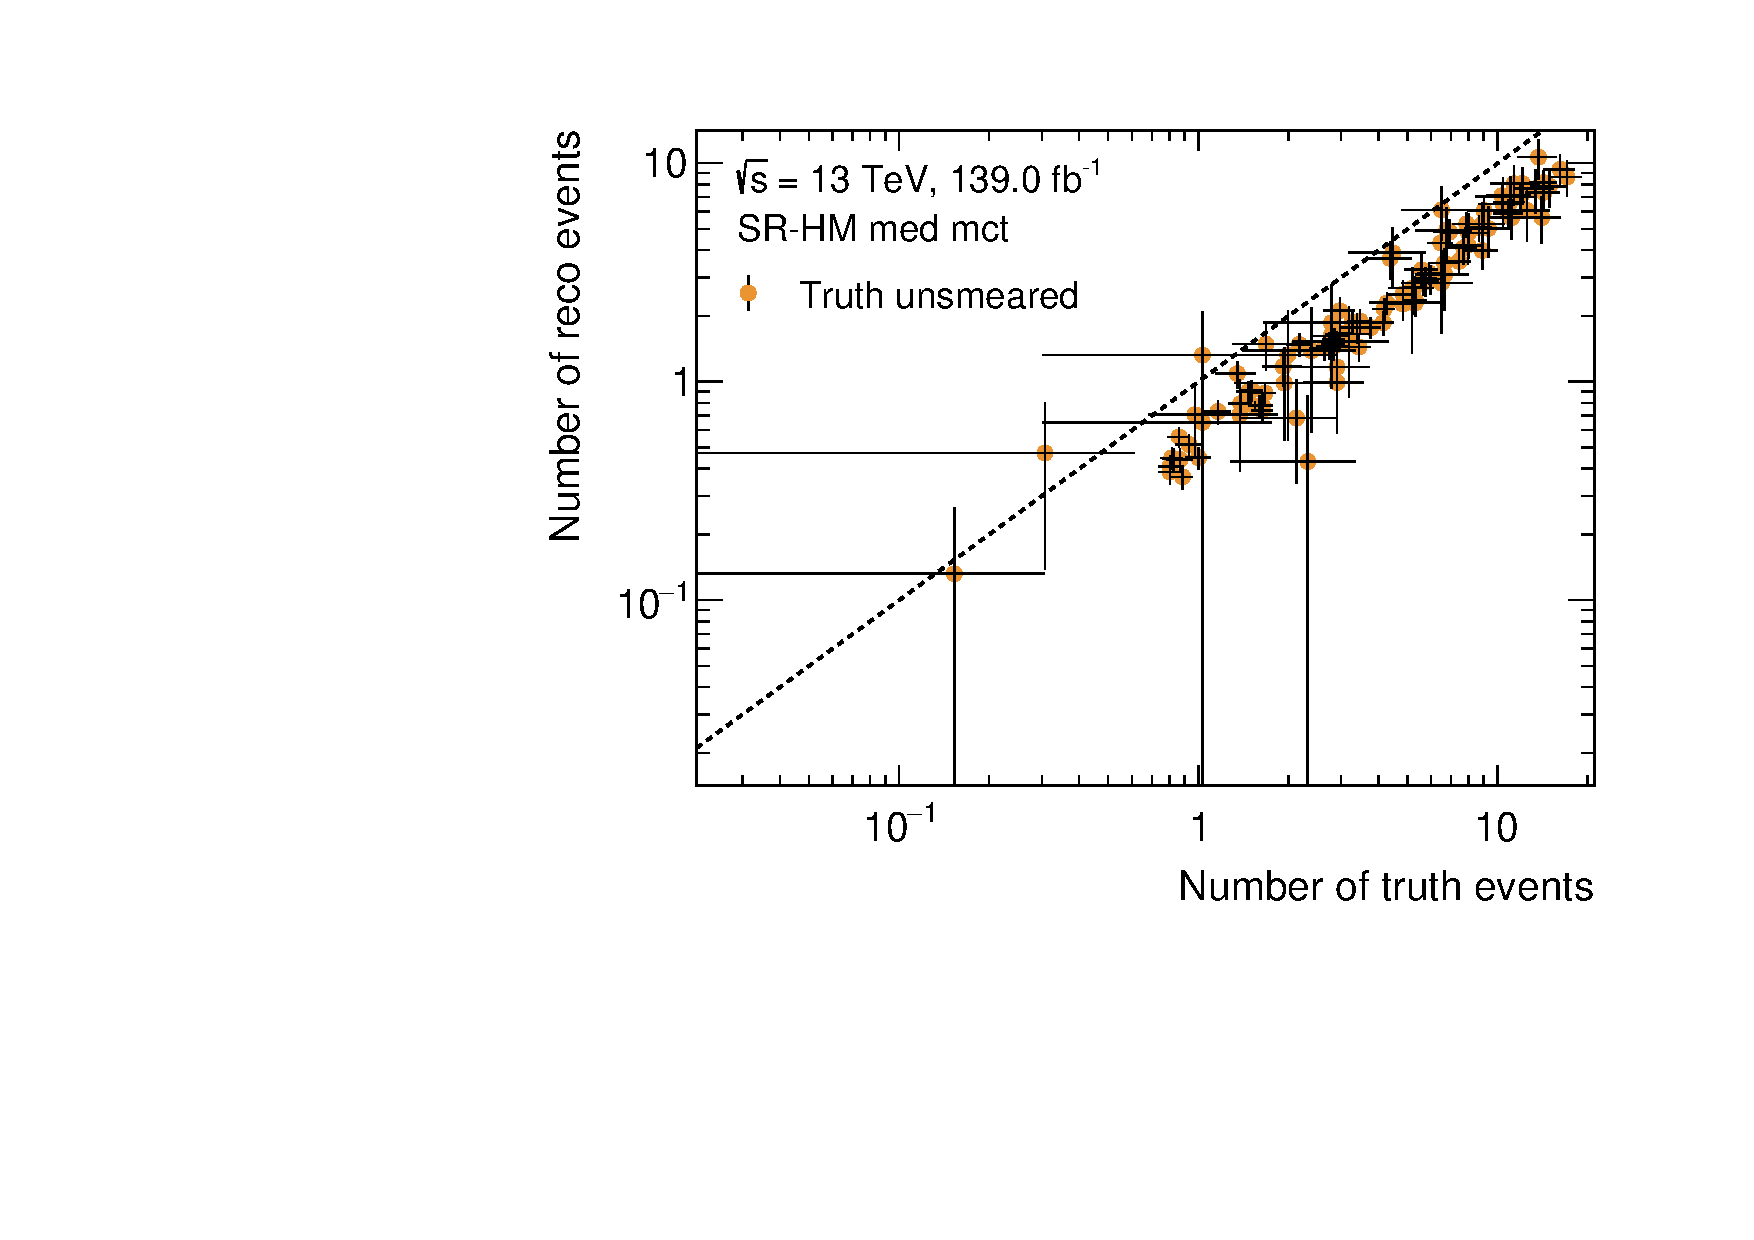
\includegraphics[width=\textwidth]{yields_SR-HM_med_mct_unsmeared}
	\end{subfigure}\hfill
	\begin{subfigure}[b]{0.49\linewidth}
		\centering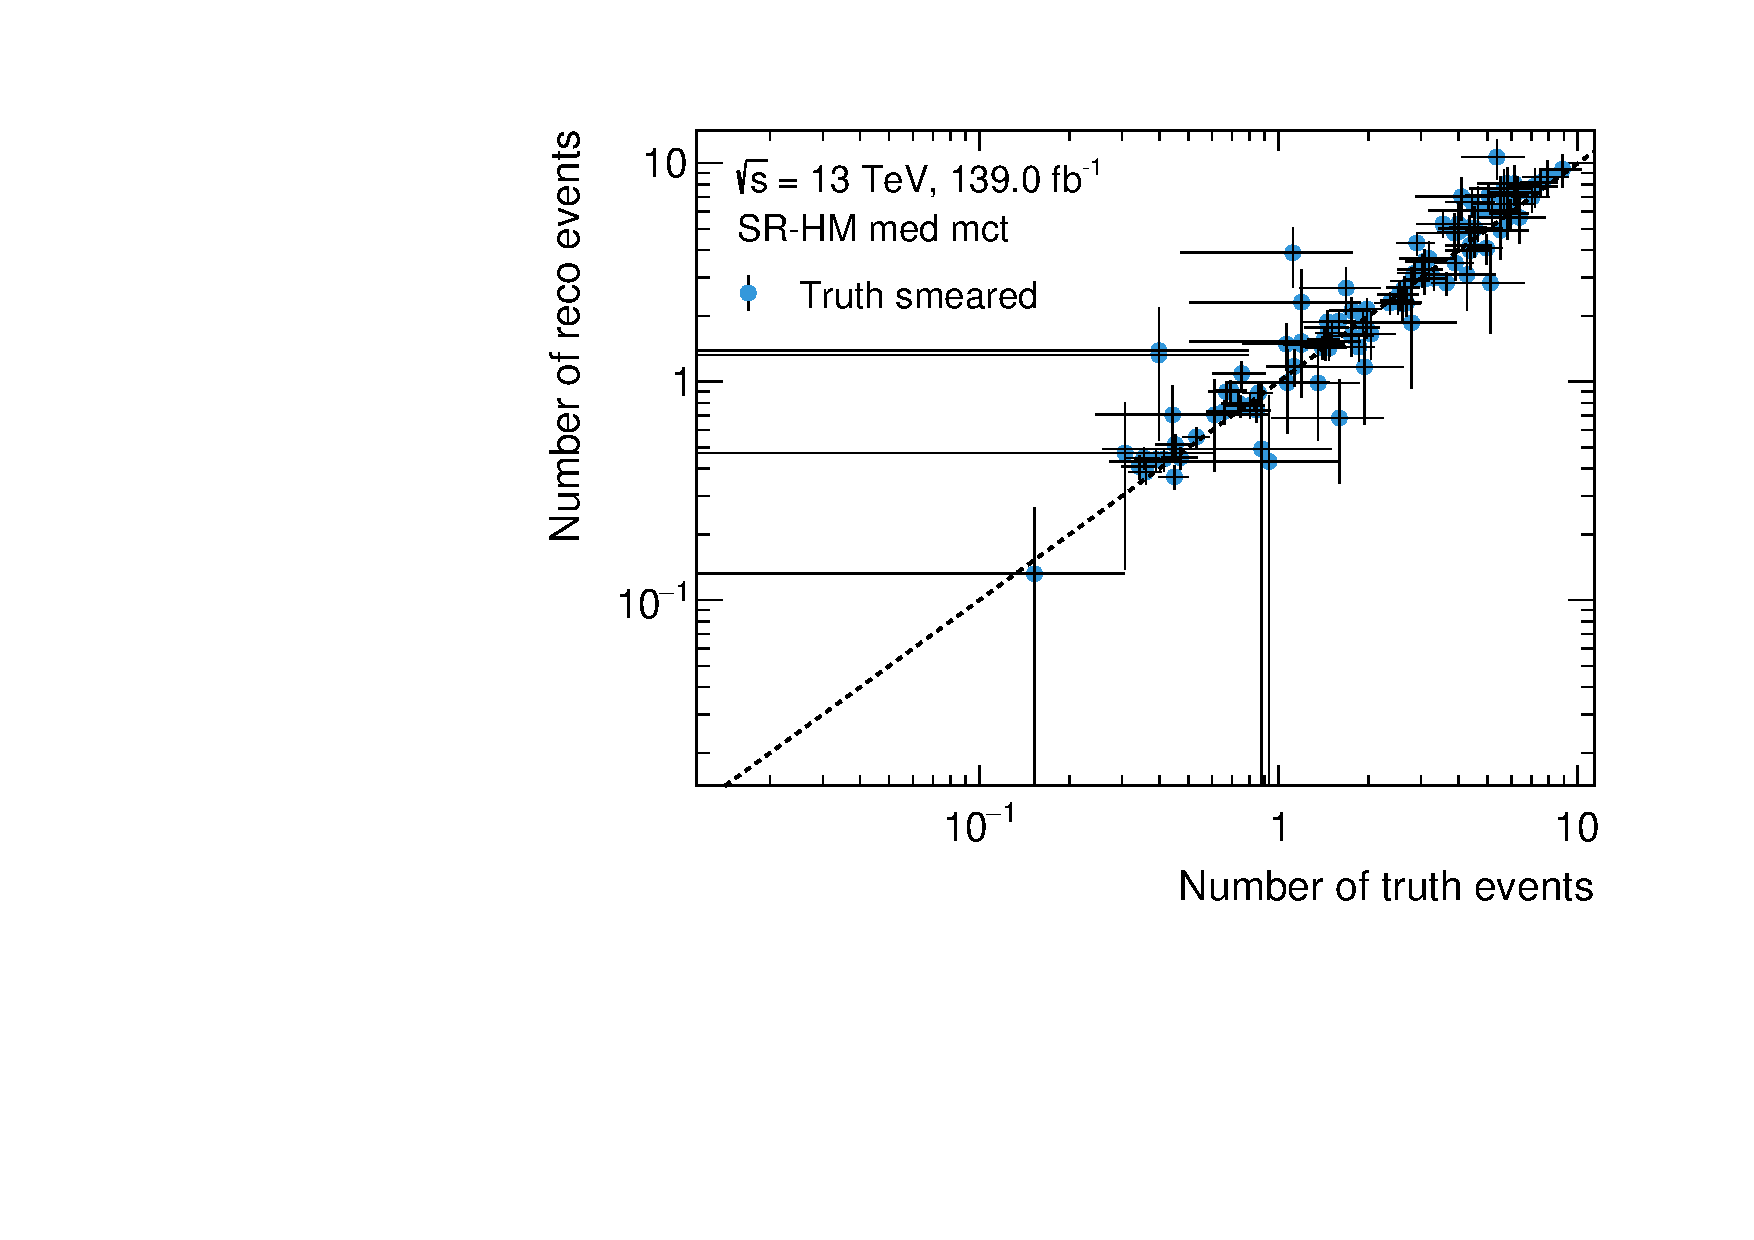
\includegraphics[width=\textwidth]{yields_SR-HM_med_mct_smeared}
	\end{subfigure}\hfill
	\begin{subfigure}[b]{0.49\linewidth}
		\centering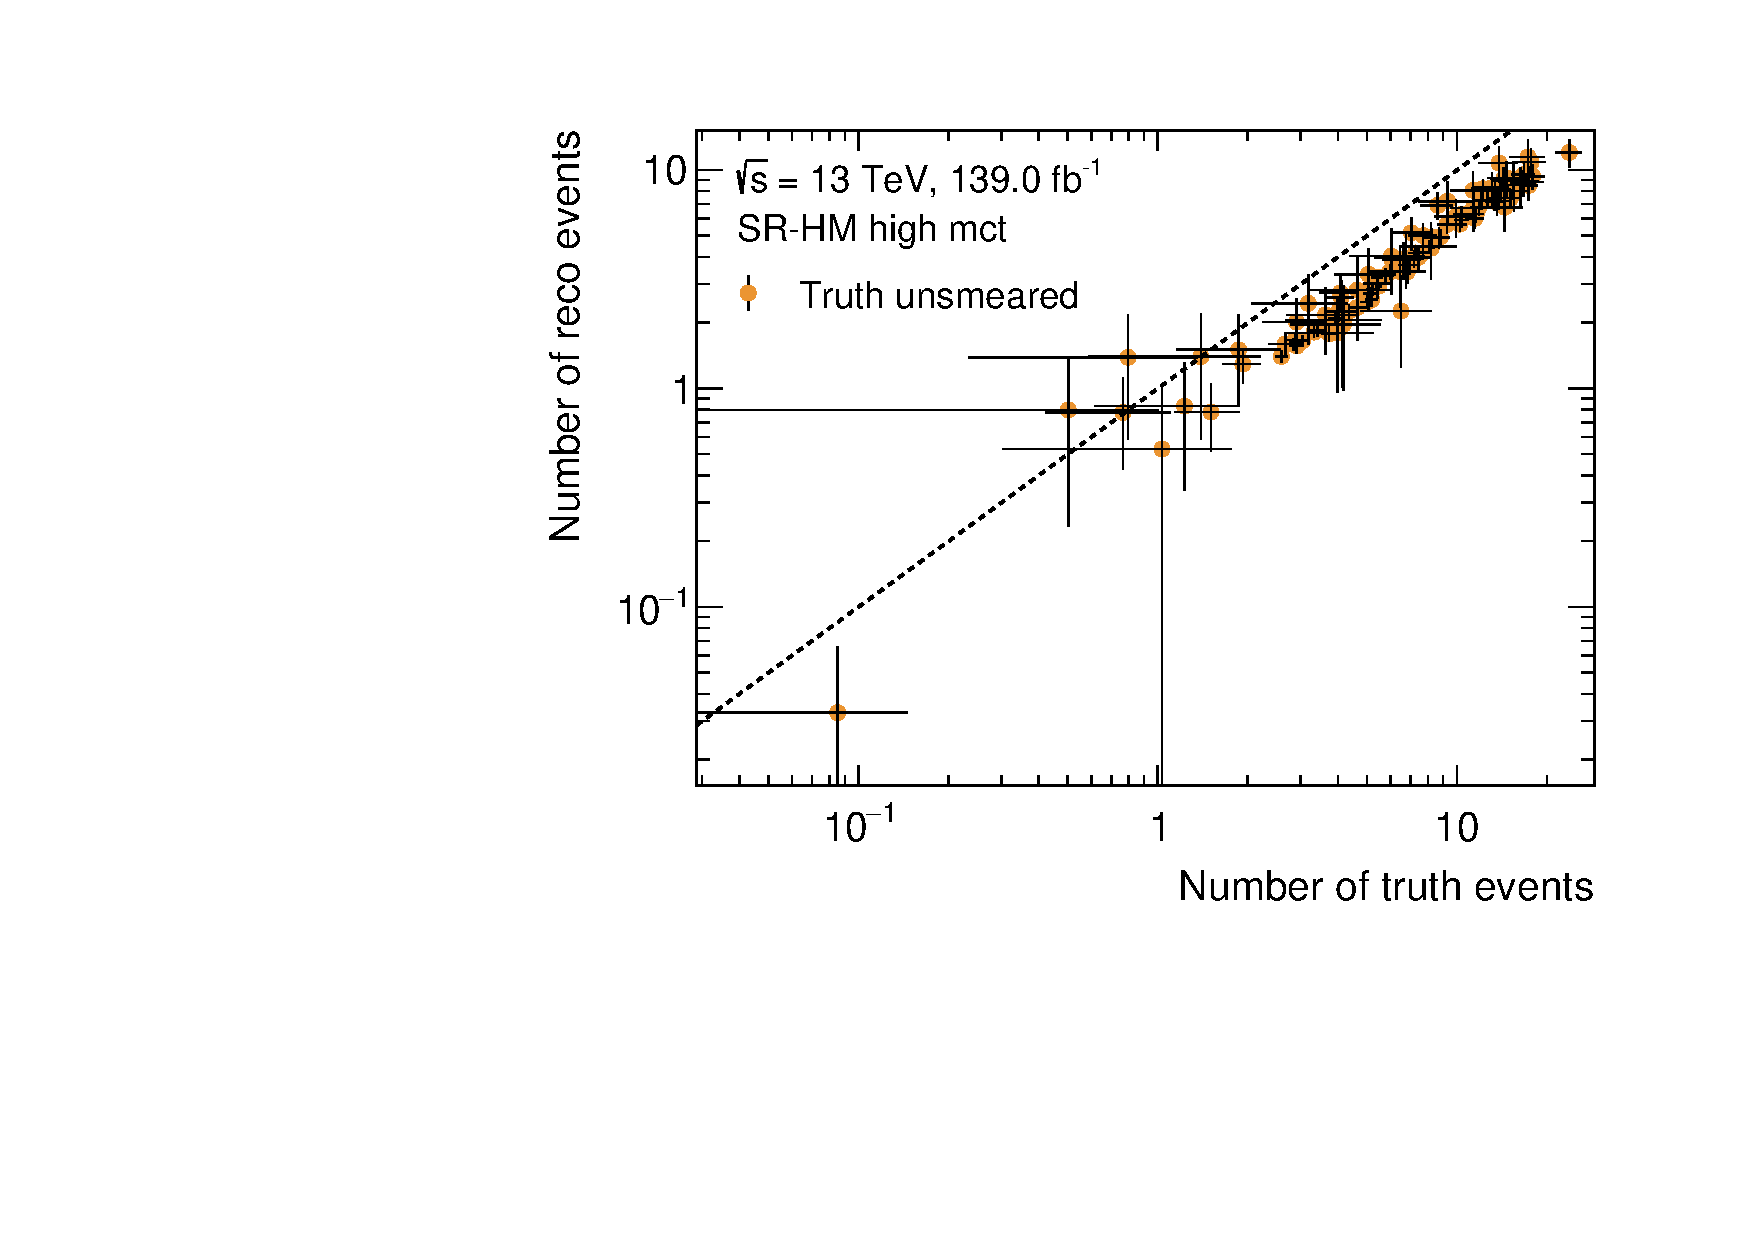
\includegraphics[width=\textwidth]{yields_SR-HM_high_mct_unsmeared}
	\end{subfigure}\hfill
	\begin{subfigure}[b]{0.49\linewidth}
		\centering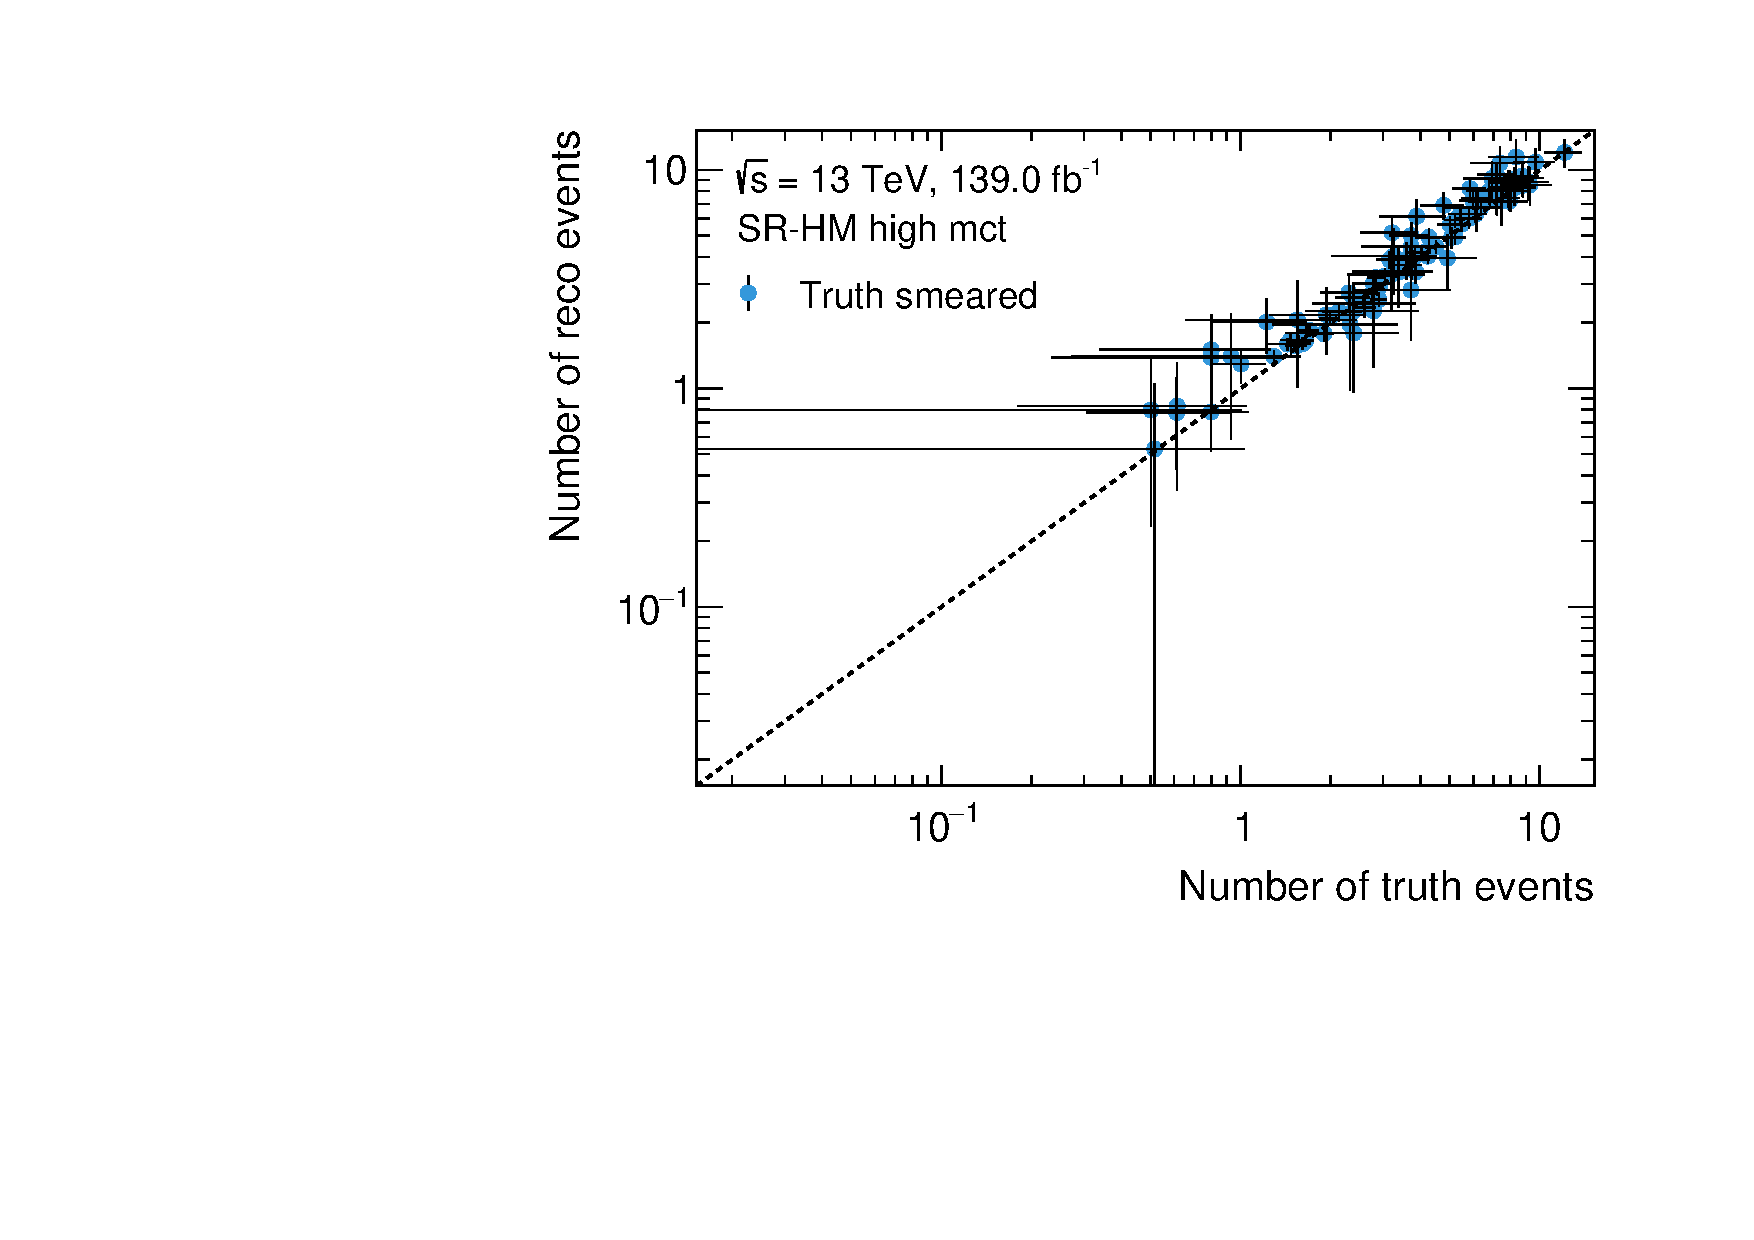
\includegraphics[width=\textwidth]{yields_SR-HM_high_mct_smeared}
	\end{subfigure}
	\caption{Comparison of the event rates at truth- and reconstruction-level before (left) and after (right) truth smearing in SR-HM. From top to bottom, the low, medium and high $\mct$ bins are shown. Every single point in the scatter plots represents a single signal model considered in the original 1-lepton analysis. Uncertainties include only \gls{mc} statistical uncertainties.}
	\label{fig:smearing_signal_regions_3}
\end{figure}


\section{Impact of LSP type}

 \begin{figure}
	\centering
	\begin{subfigure}[b]{0.5\linewidth}
		\centering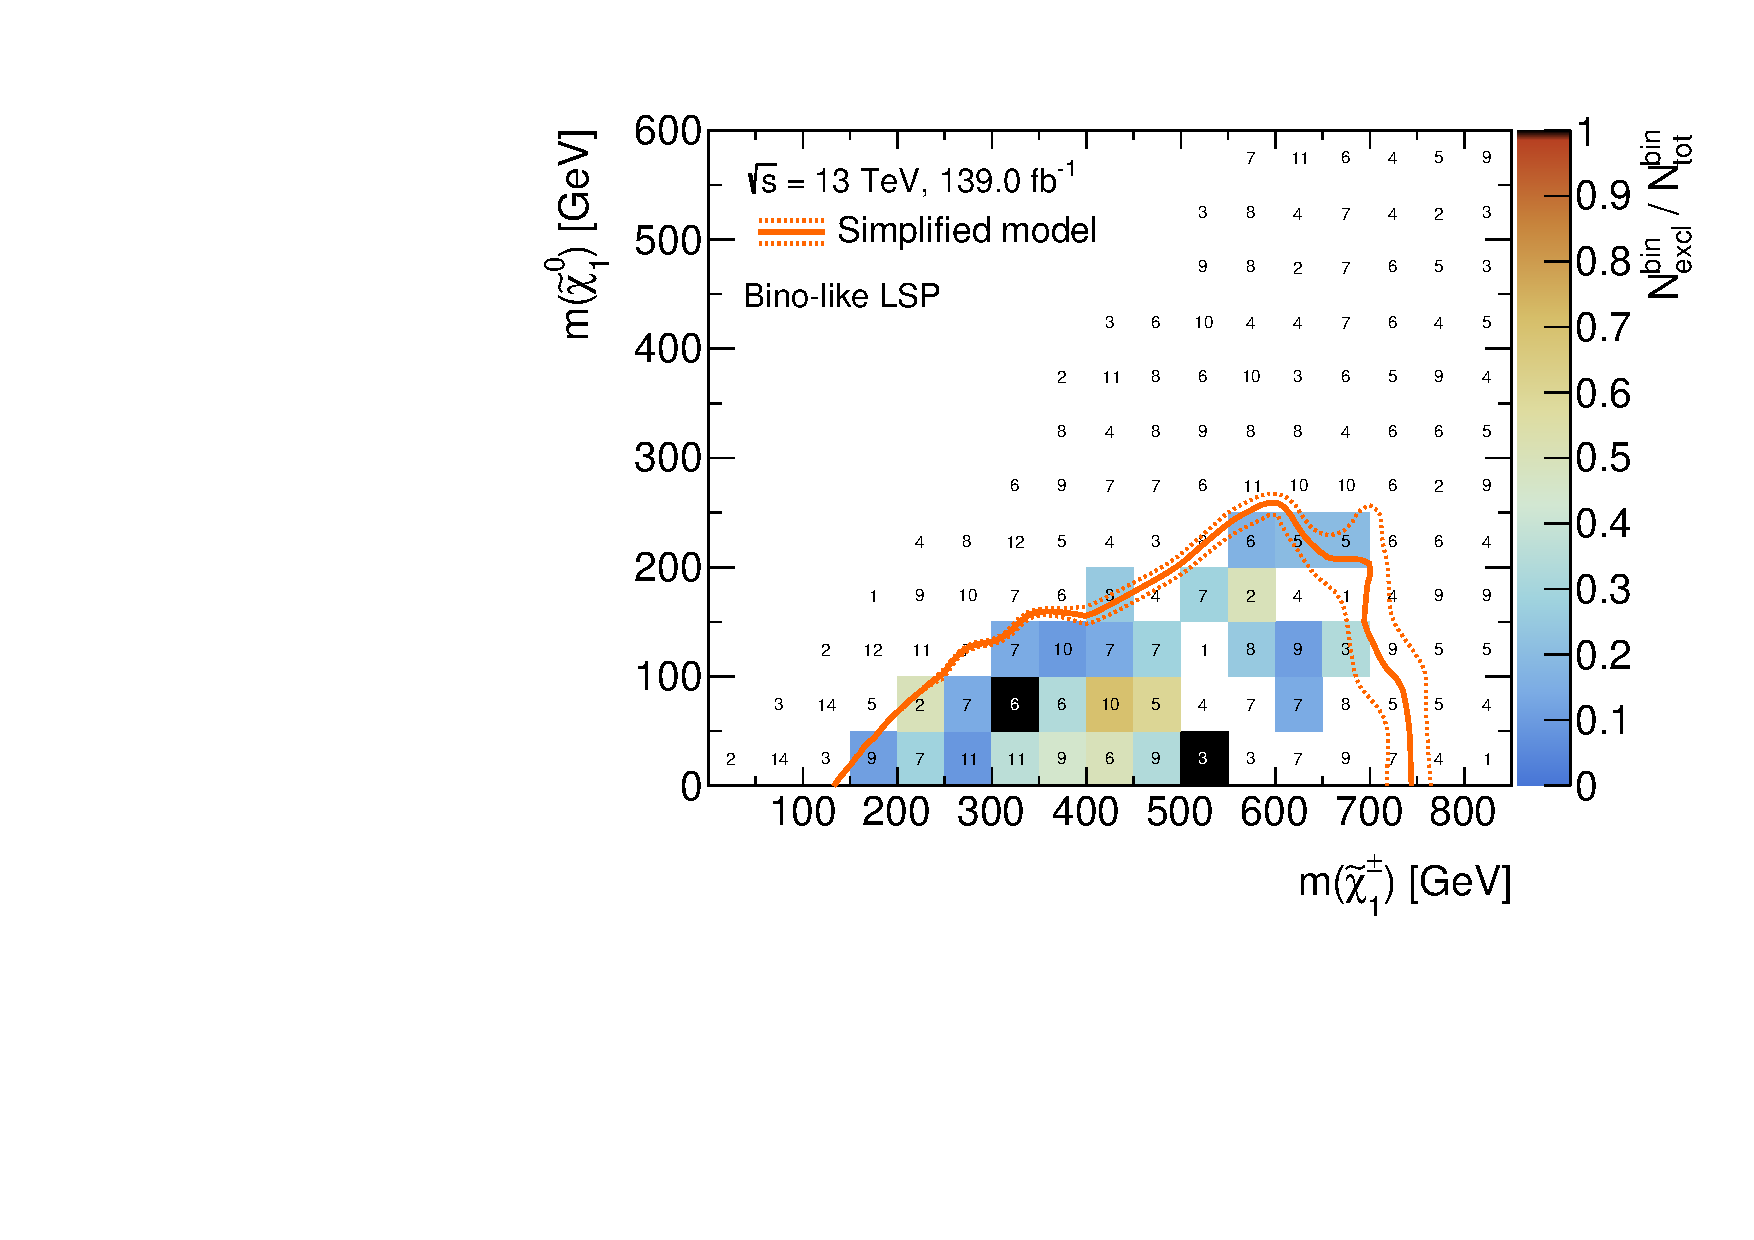
\includegraphics[width=\textwidth]{cut_bino_LSP/mchi1p_mlsp_contour}
		\caption{\label{fig:mchi1p_mlsp_contour_bino_lsp}}
	\end{subfigure}\hfill
	\begin{subfigure}[b]{0.5\linewidth}
		\centering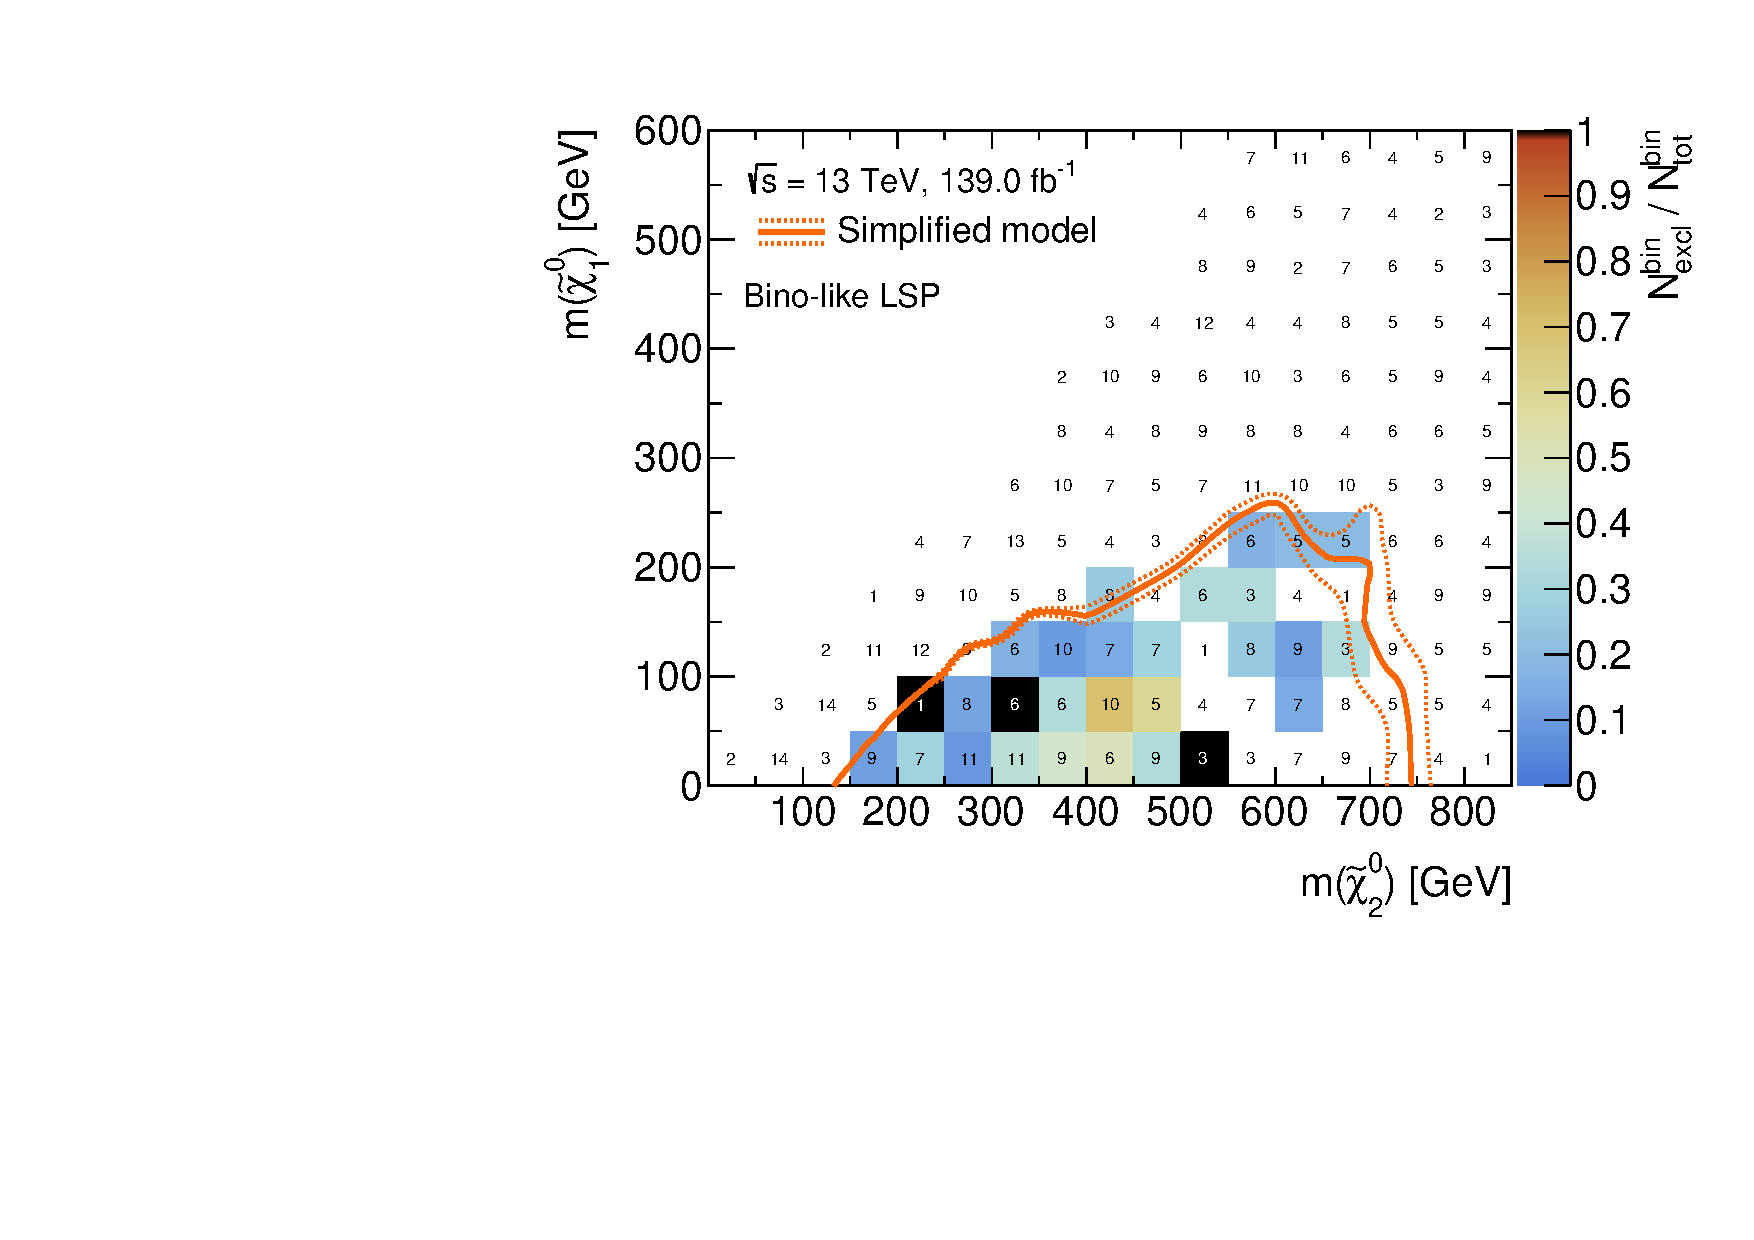
\includegraphics[width=\textwidth]{cut_bino_LSP/mchi20_mlsp_contour}
		\caption{\label{fig:mchi20_mlsp_contour_bino_lsp}}
	\end{subfigure}\hfill
	\begin{subfigure}[b]{0.5\linewidth}
		\centering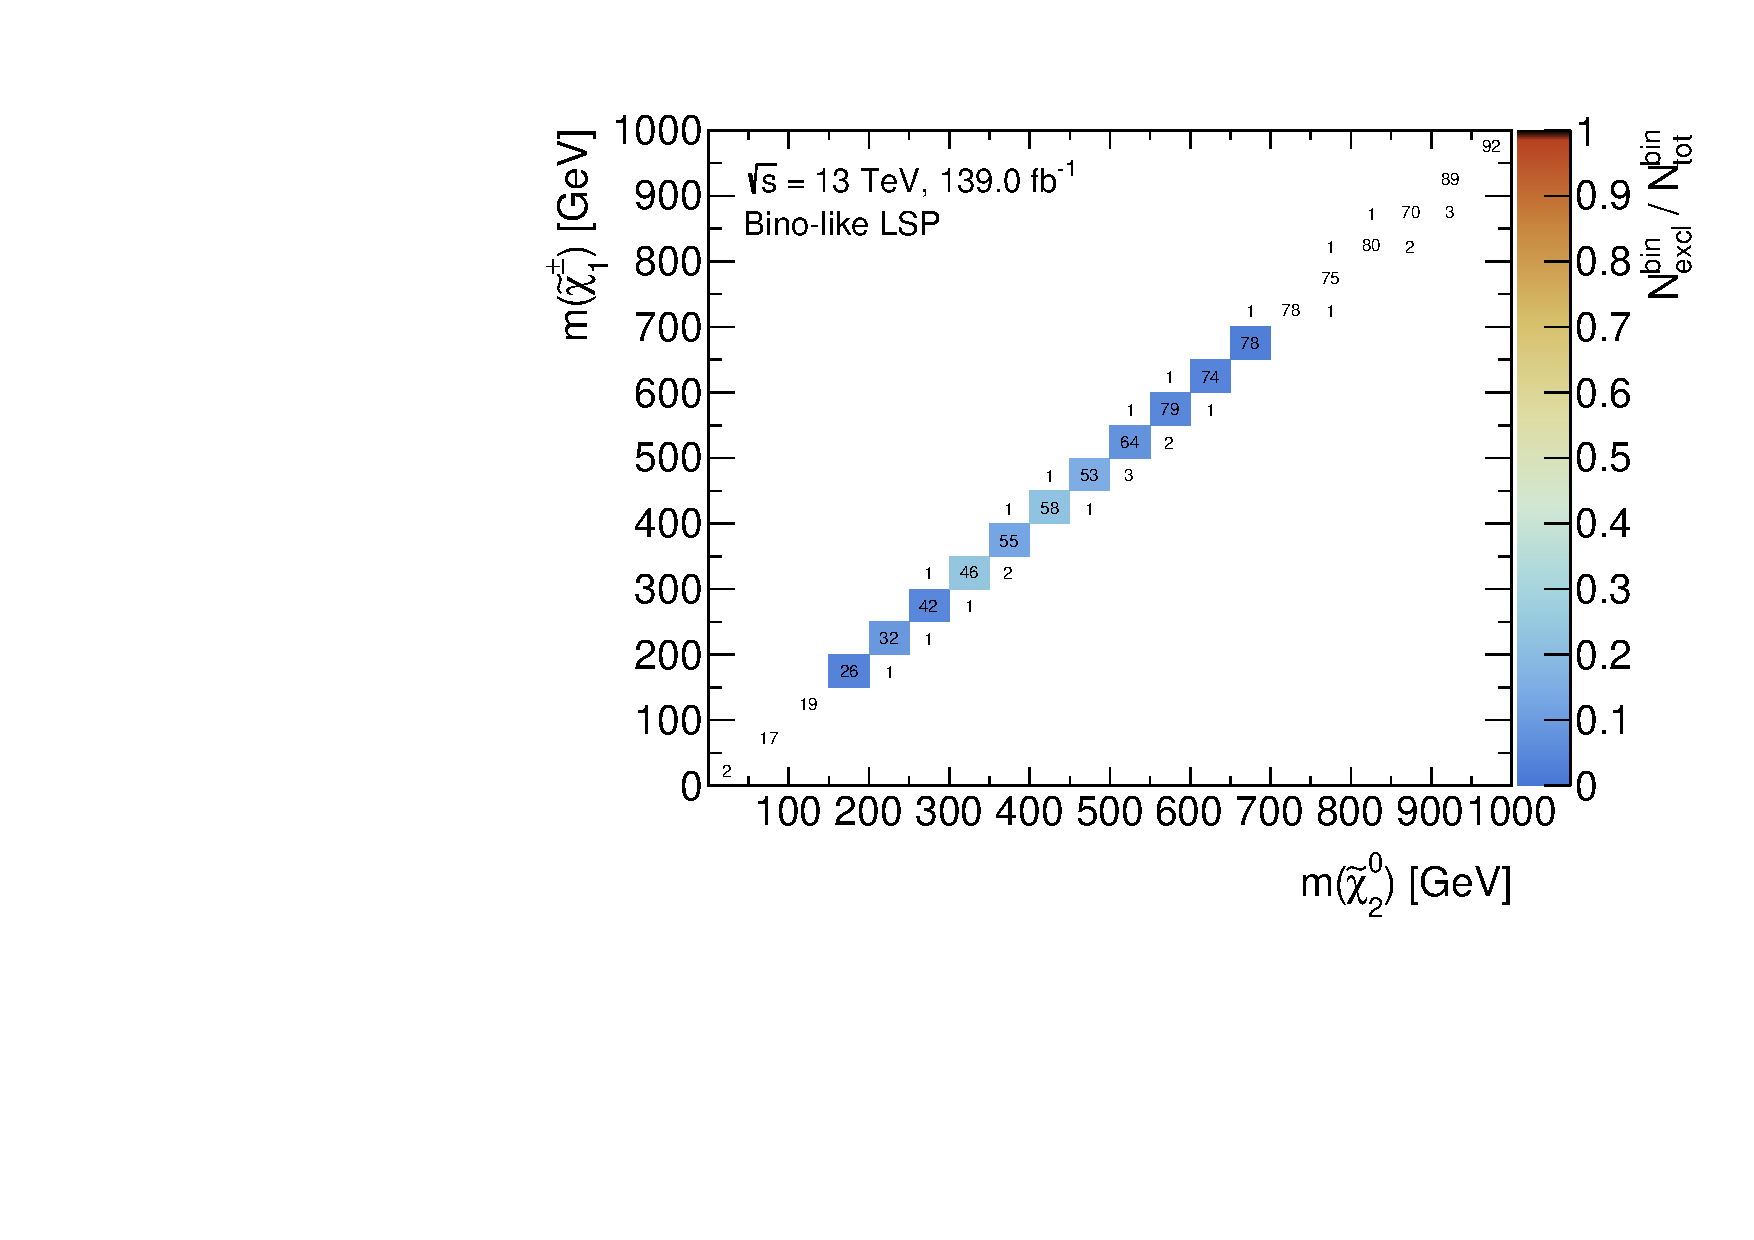
\includegraphics[width=\textwidth]{cut_bino_LSP/mchi1p_mchi20_contour}
		\caption{\label{fig:mchi1p_mchi20_contour_bino_lsp}}
	\end{subfigure}\hfill
	\caption{Bin-by-bin fraction of excluded models as a function of the relevant sparticle masses. Only \gls{pmssm} models with a bino-like \gls{lsp} are shown. The numbers in the bins correspond to the total number of models sampled falling into the respective bin. The number of models excluded by the 1-lepton analysis is encoded with a colour bar ranging from 0 to 1. Where all models in a given bin are excluded, the bin is coloured in black. Bins without a models excluded are left white. Models are evaluated using the simplified likelihood of the 1-lepton analysis. The simplified model contour is shown in orange.}
	\label{fig:impact_electroweakinos_2D_bino_lsp}
\end{figure}

 \begin{figure}
	\centering
	\begin{subfigure}[b]{0.5\linewidth}
		\centering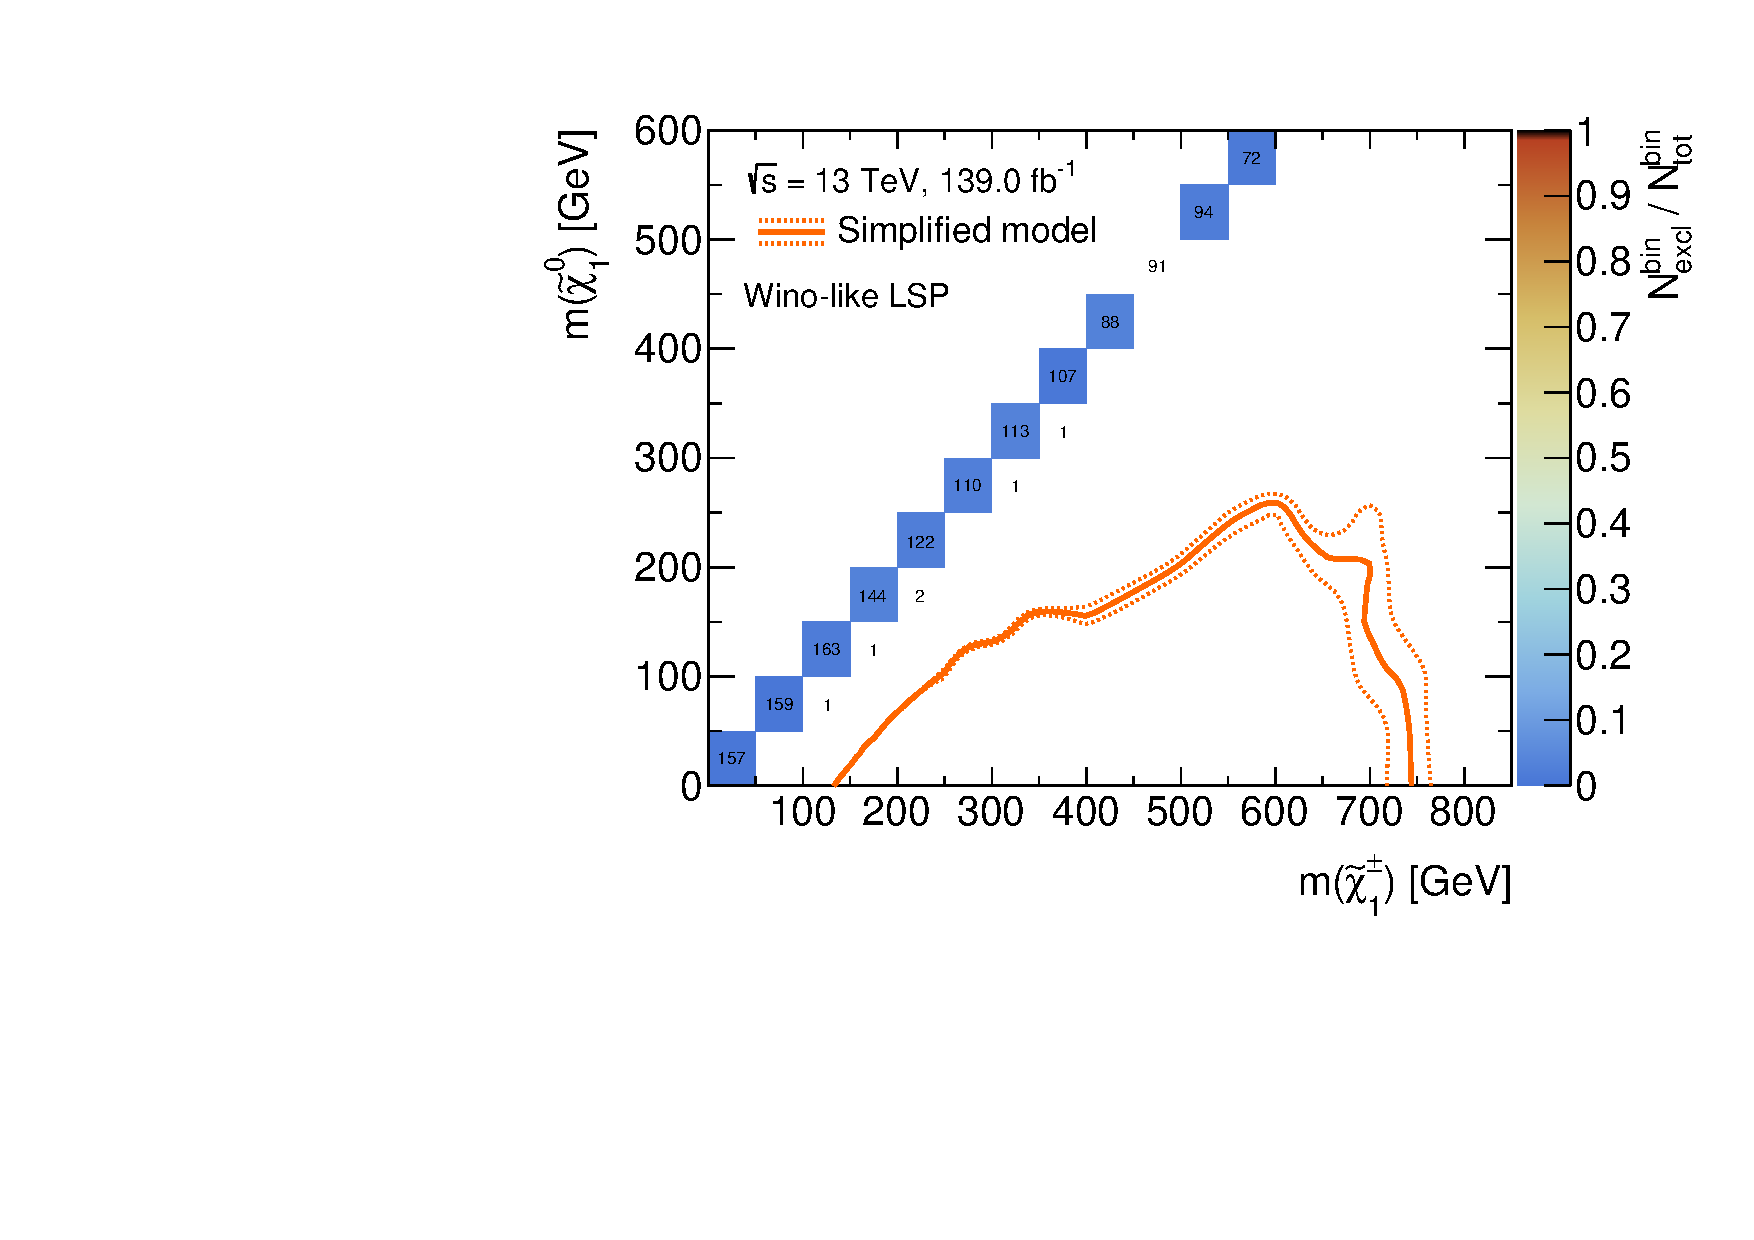
\includegraphics[width=\textwidth]{cut_wino_LSP/mchi1p_mlsp_contour}
		\caption{\label{fig:mchi1p_mlsp_contour_wino_lsp}}
	\end{subfigure}\hfill
	\begin{subfigure}[b]{0.5\linewidth}
		\centering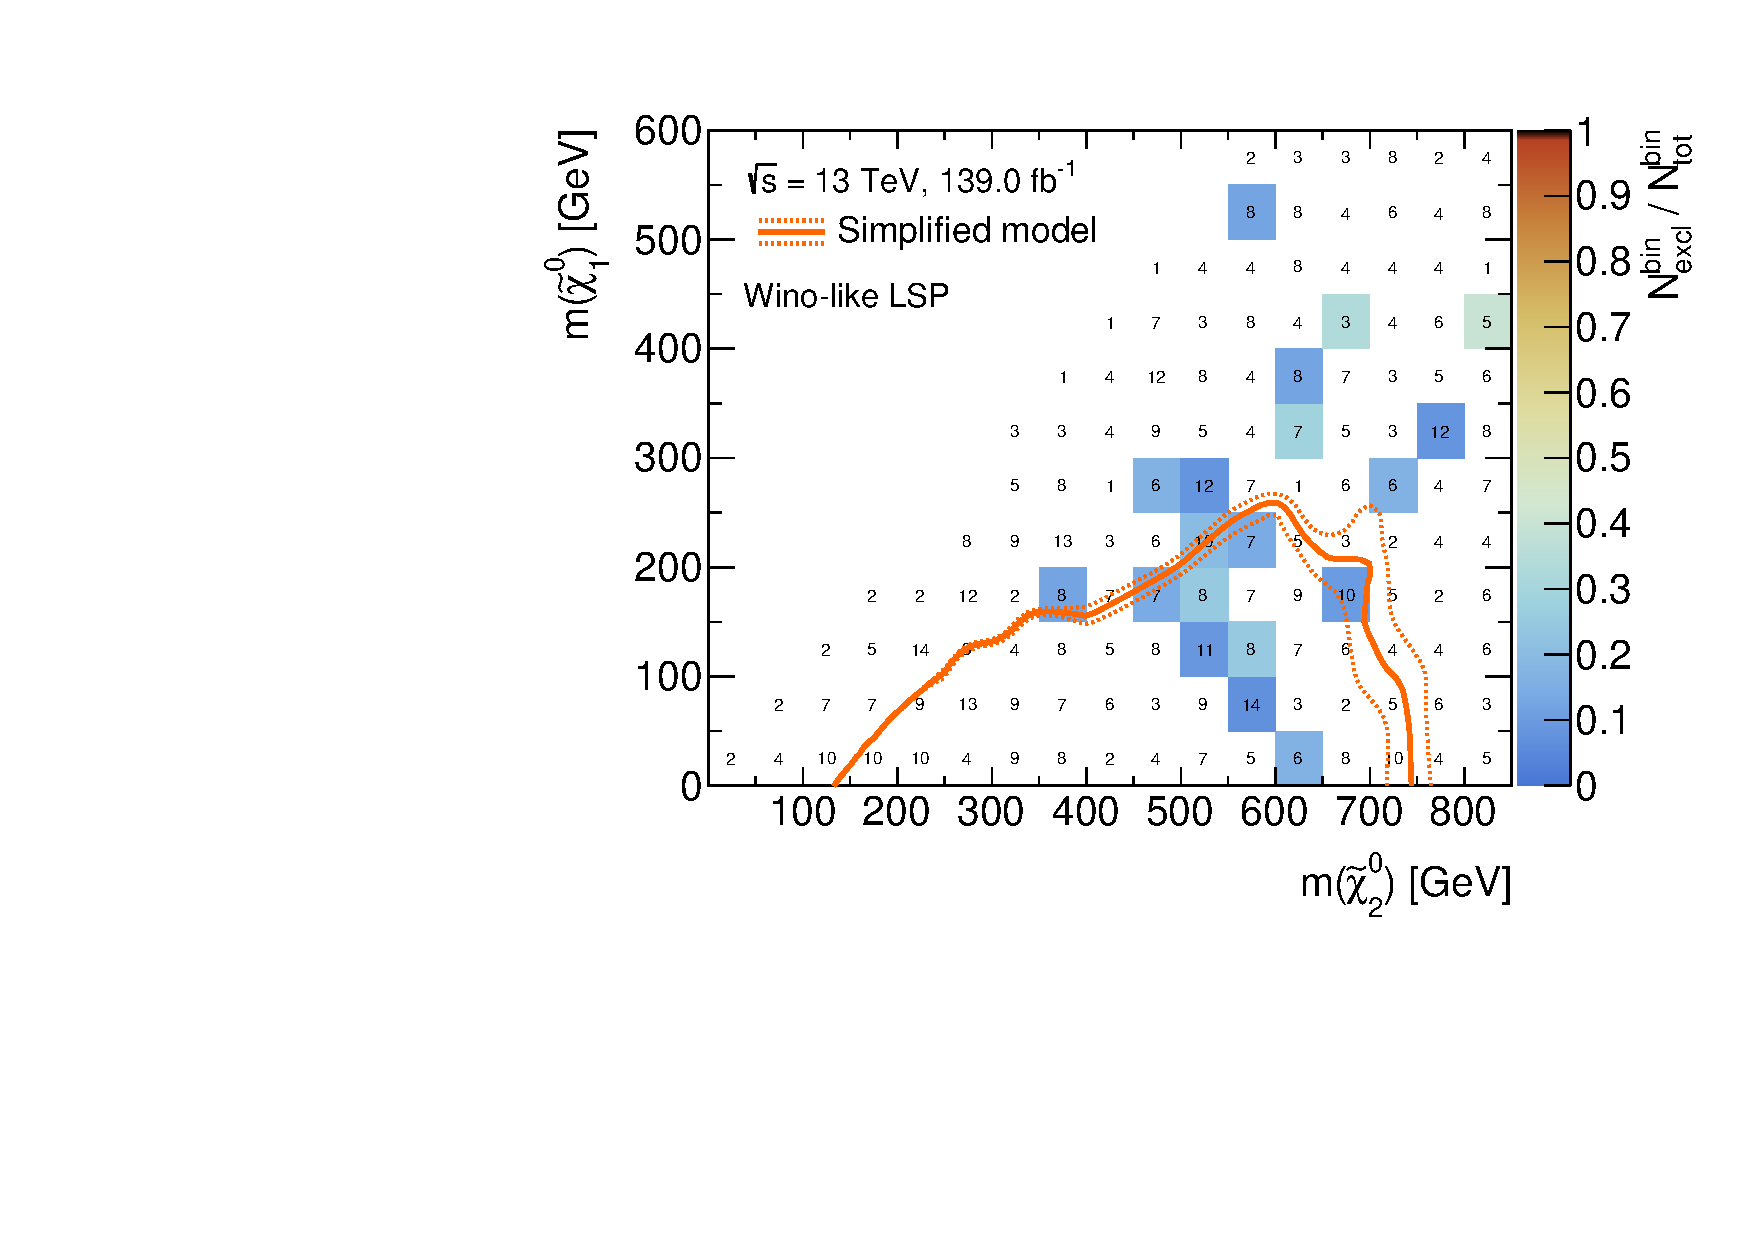
\includegraphics[width=\textwidth]{cut_wino_LSP/mchi20_mlsp_contour}
		\caption{\label{fig:mchi20_mlsp_contour_wino_lsp}}
	\end{subfigure}\hfill
	\begin{subfigure}[b]{0.5\linewidth}
		\centering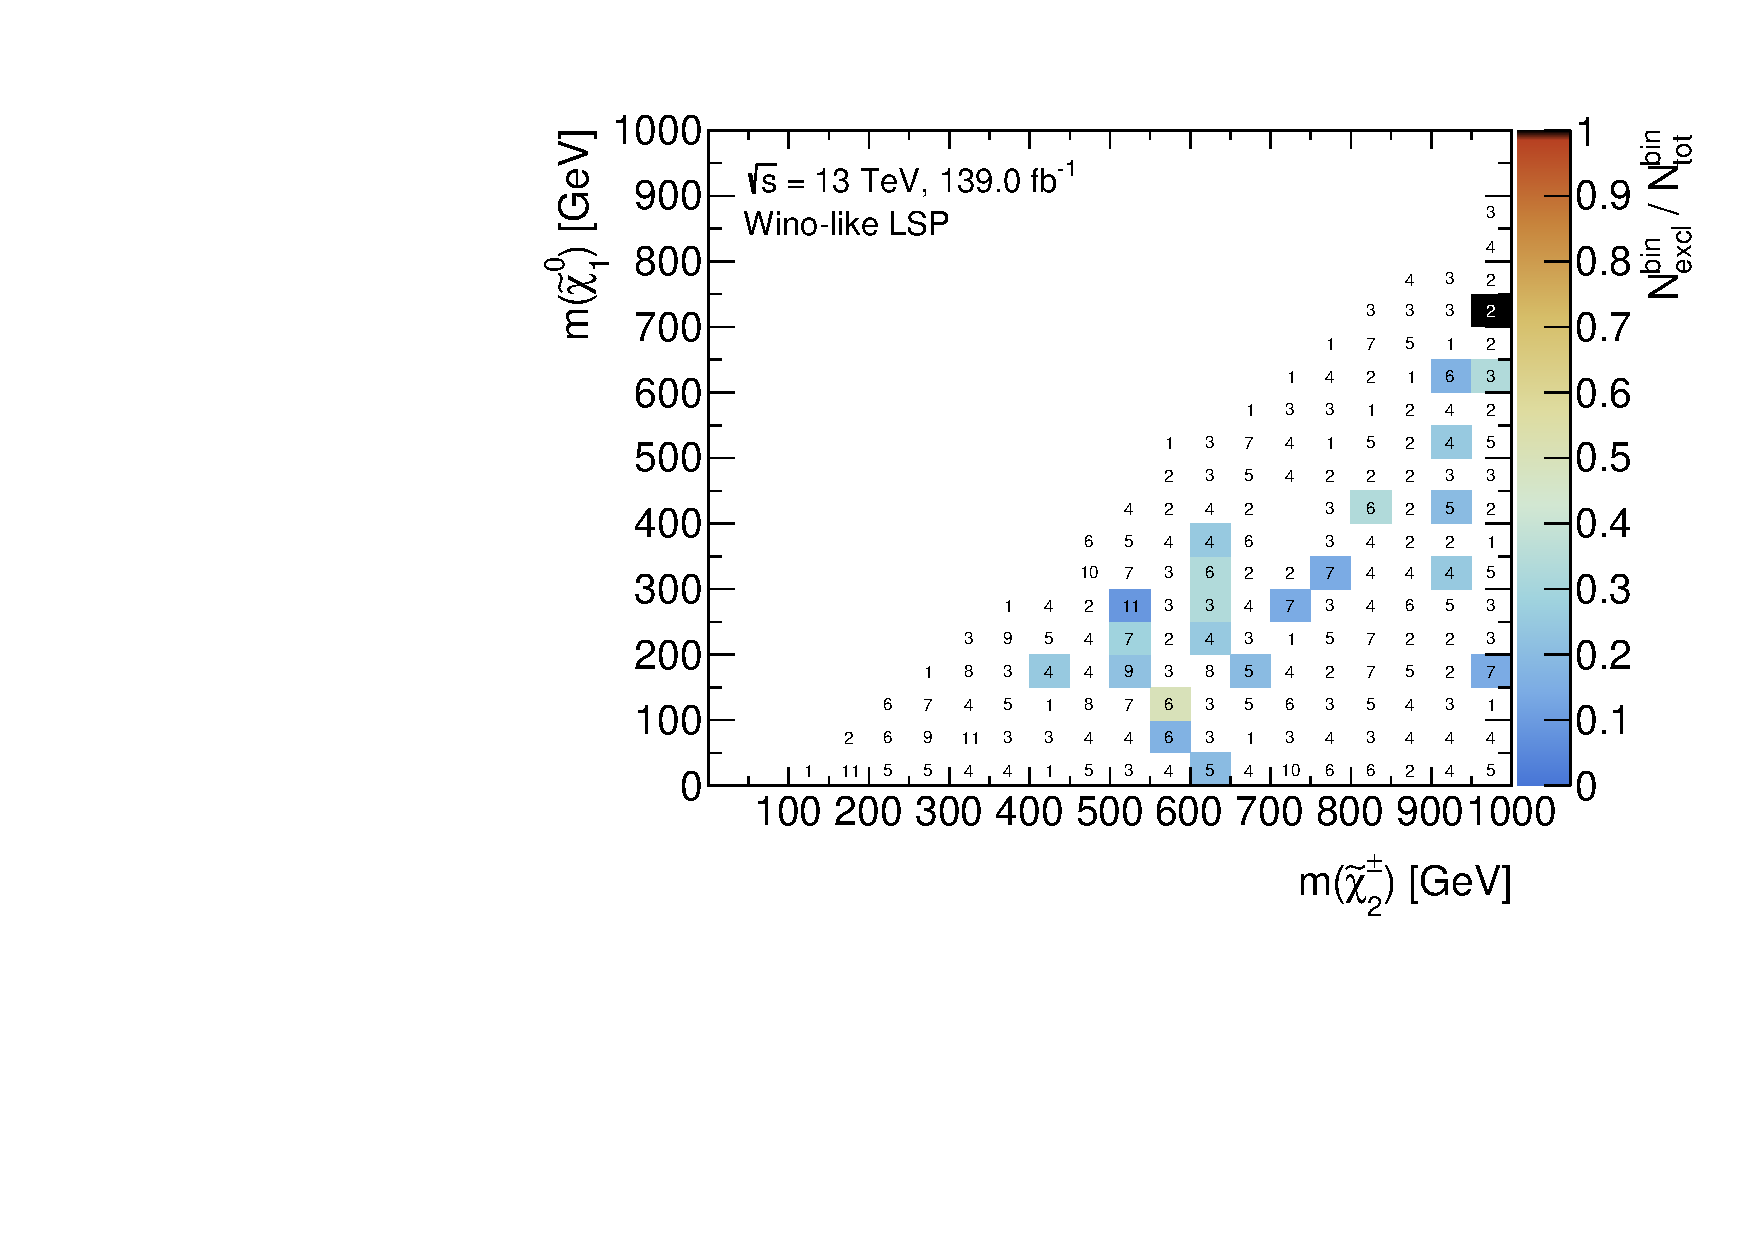
\includegraphics[width=\textwidth]{cut_wino_LSP/mchi10_mchi2p_contour}
		\caption{\label{fig:mchi10_mchi2p_contour_wino_lsp}}
	\end{subfigure}\hfill
	\caption{Bin-by-bin fraction of excluded models as a function of the relevant sparticle masses. Only \gls{pmssm} models with a wino-like \gls{lsp} are shown. The numbers in the bins correspond to the total number of models sampled falling into the respective bin. The number of models excluded by the 1-lepton analysis is encoded with a colour bar ranging from 0 to 1. Where all models in a given bin are excluded, the bin is coloured in black. Bins without a models excluded are left white. Models are evaluated using the simplified likelihood of the 1-lepton analysis. The simplified model contour is shown in orange.}
	\label{fig:impact_electroweakinos_2D_wino_lsp}
\end{figure}

 \begin{figure}
	\centering
	\begin{subfigure}[b]{0.5\linewidth}
		\centering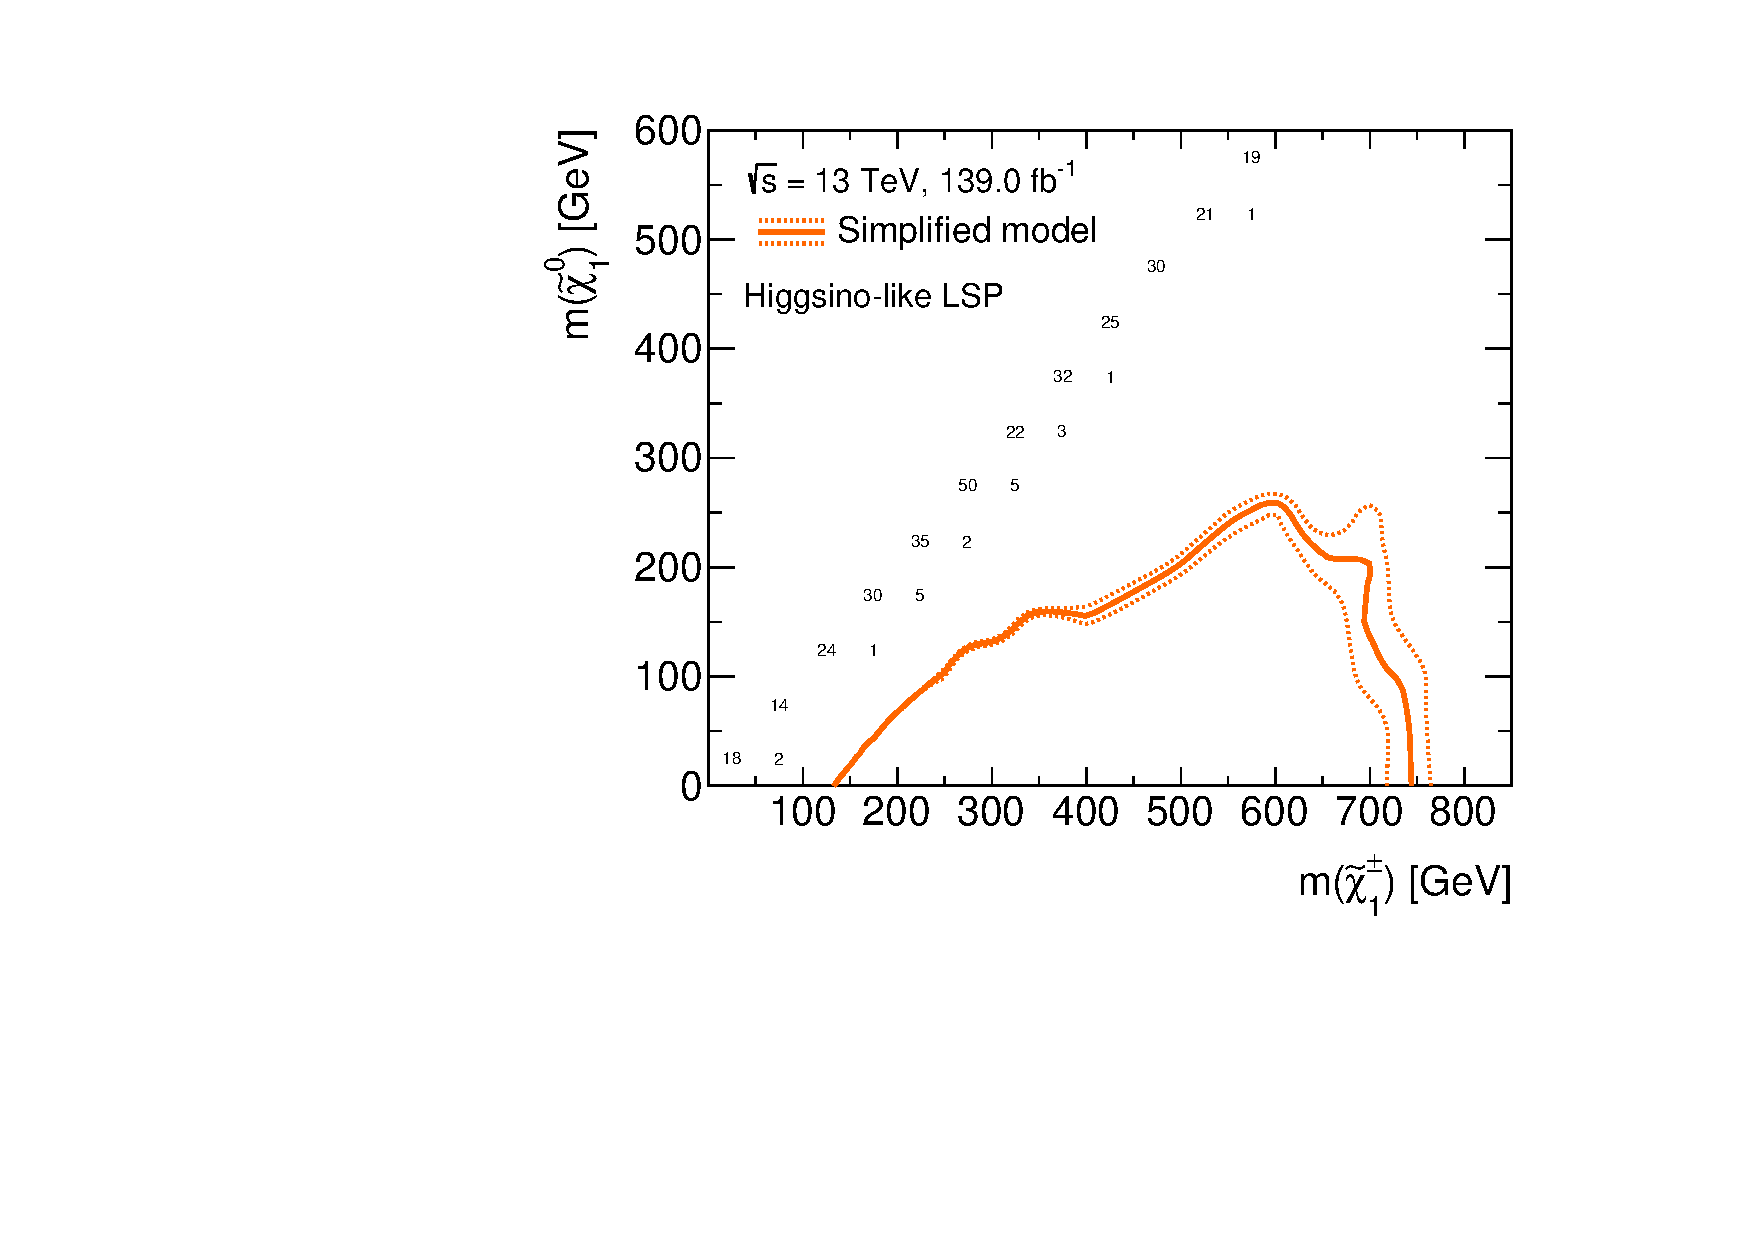
\includegraphics[width=\textwidth]{cut_higgsino_LSP/mchi1p_mlsp_contour}
		\caption{\label{fig:mchi1p_mlsp_contour_higgsino_lsp}}
	\end{subfigure}\hfill
	\begin{subfigure}[b]{0.5\linewidth}
		\centering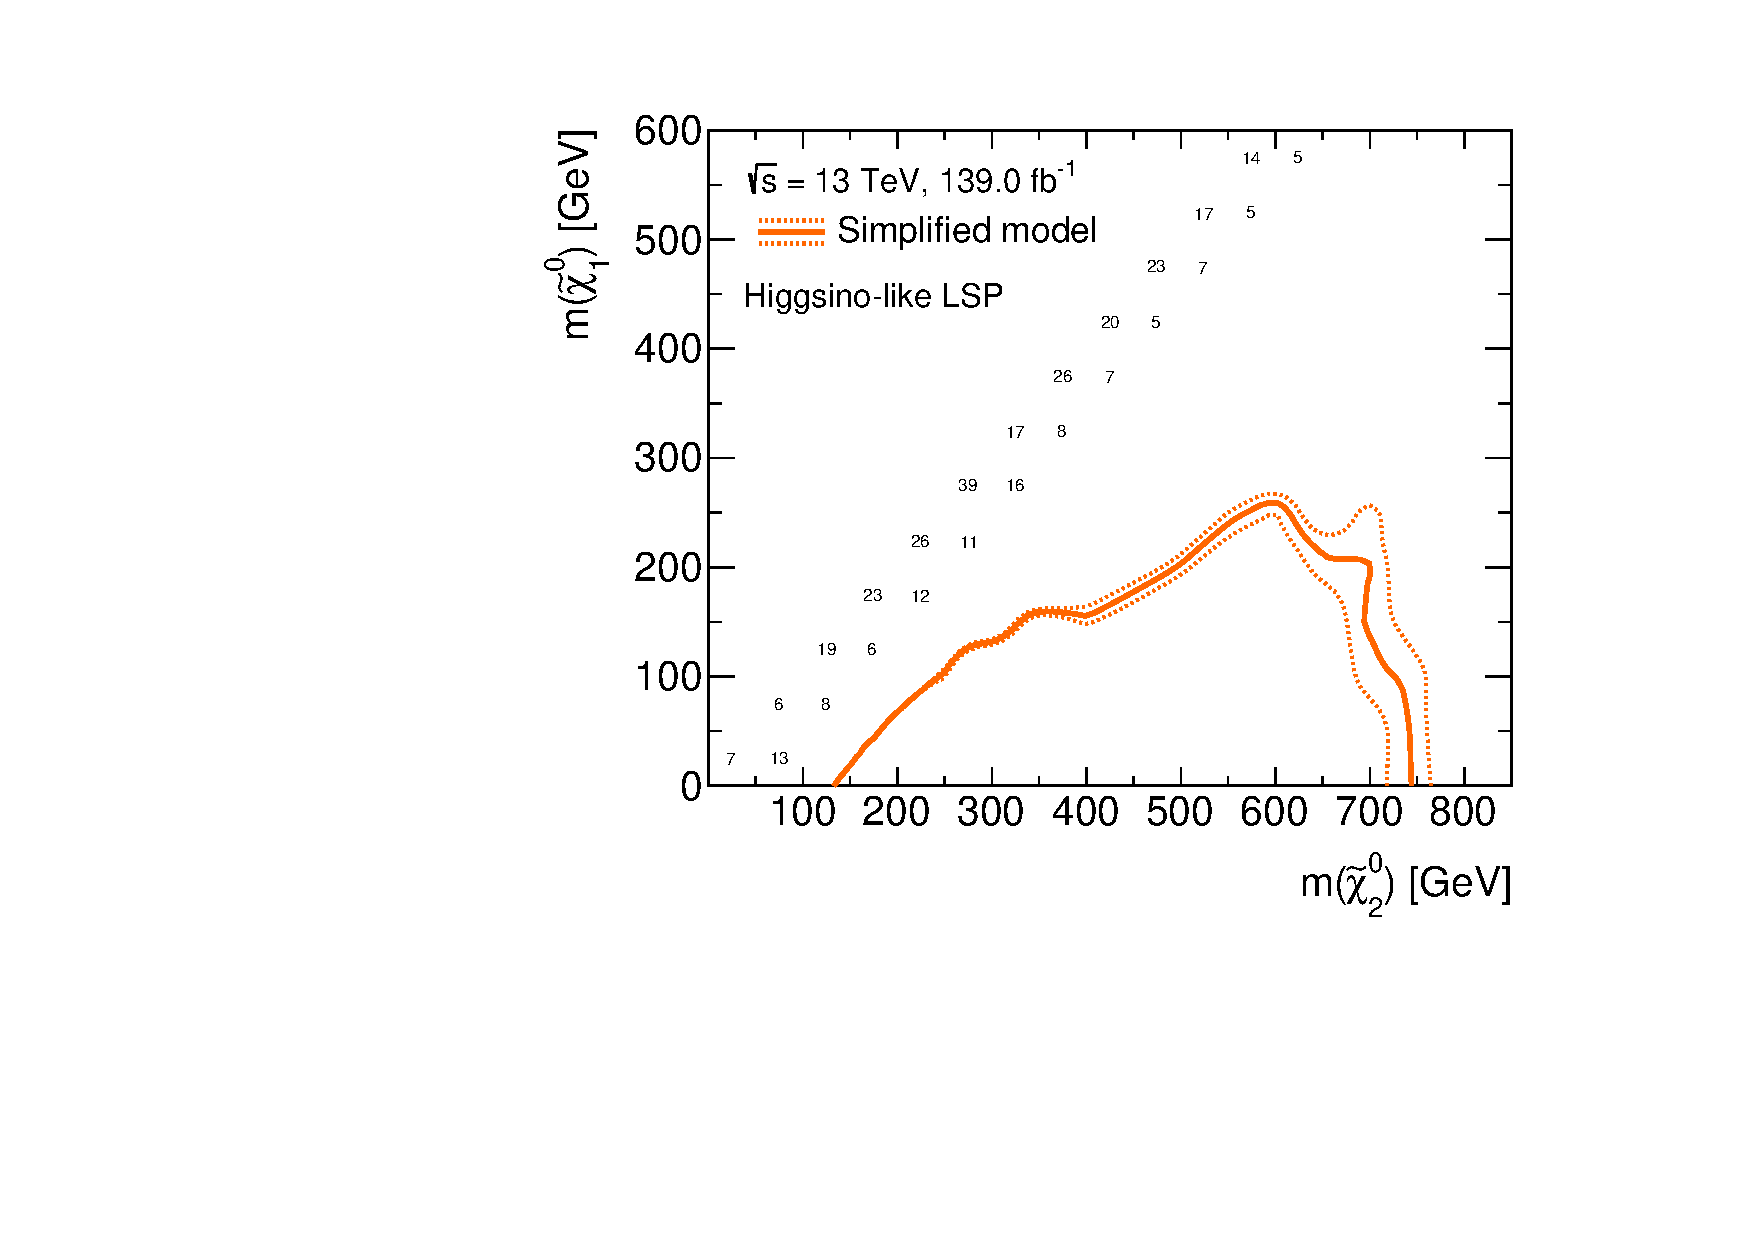
\includegraphics[width=\textwidth]{cut_higgsino_LSP/mchi20_mlsp_contour}
		\caption{\label{fig:mchi20_mlsp_contour_higgsino_lsp}}
	\end{subfigure}\hfill
	\begin{subfigure}[b]{0.5\linewidth}
		\centering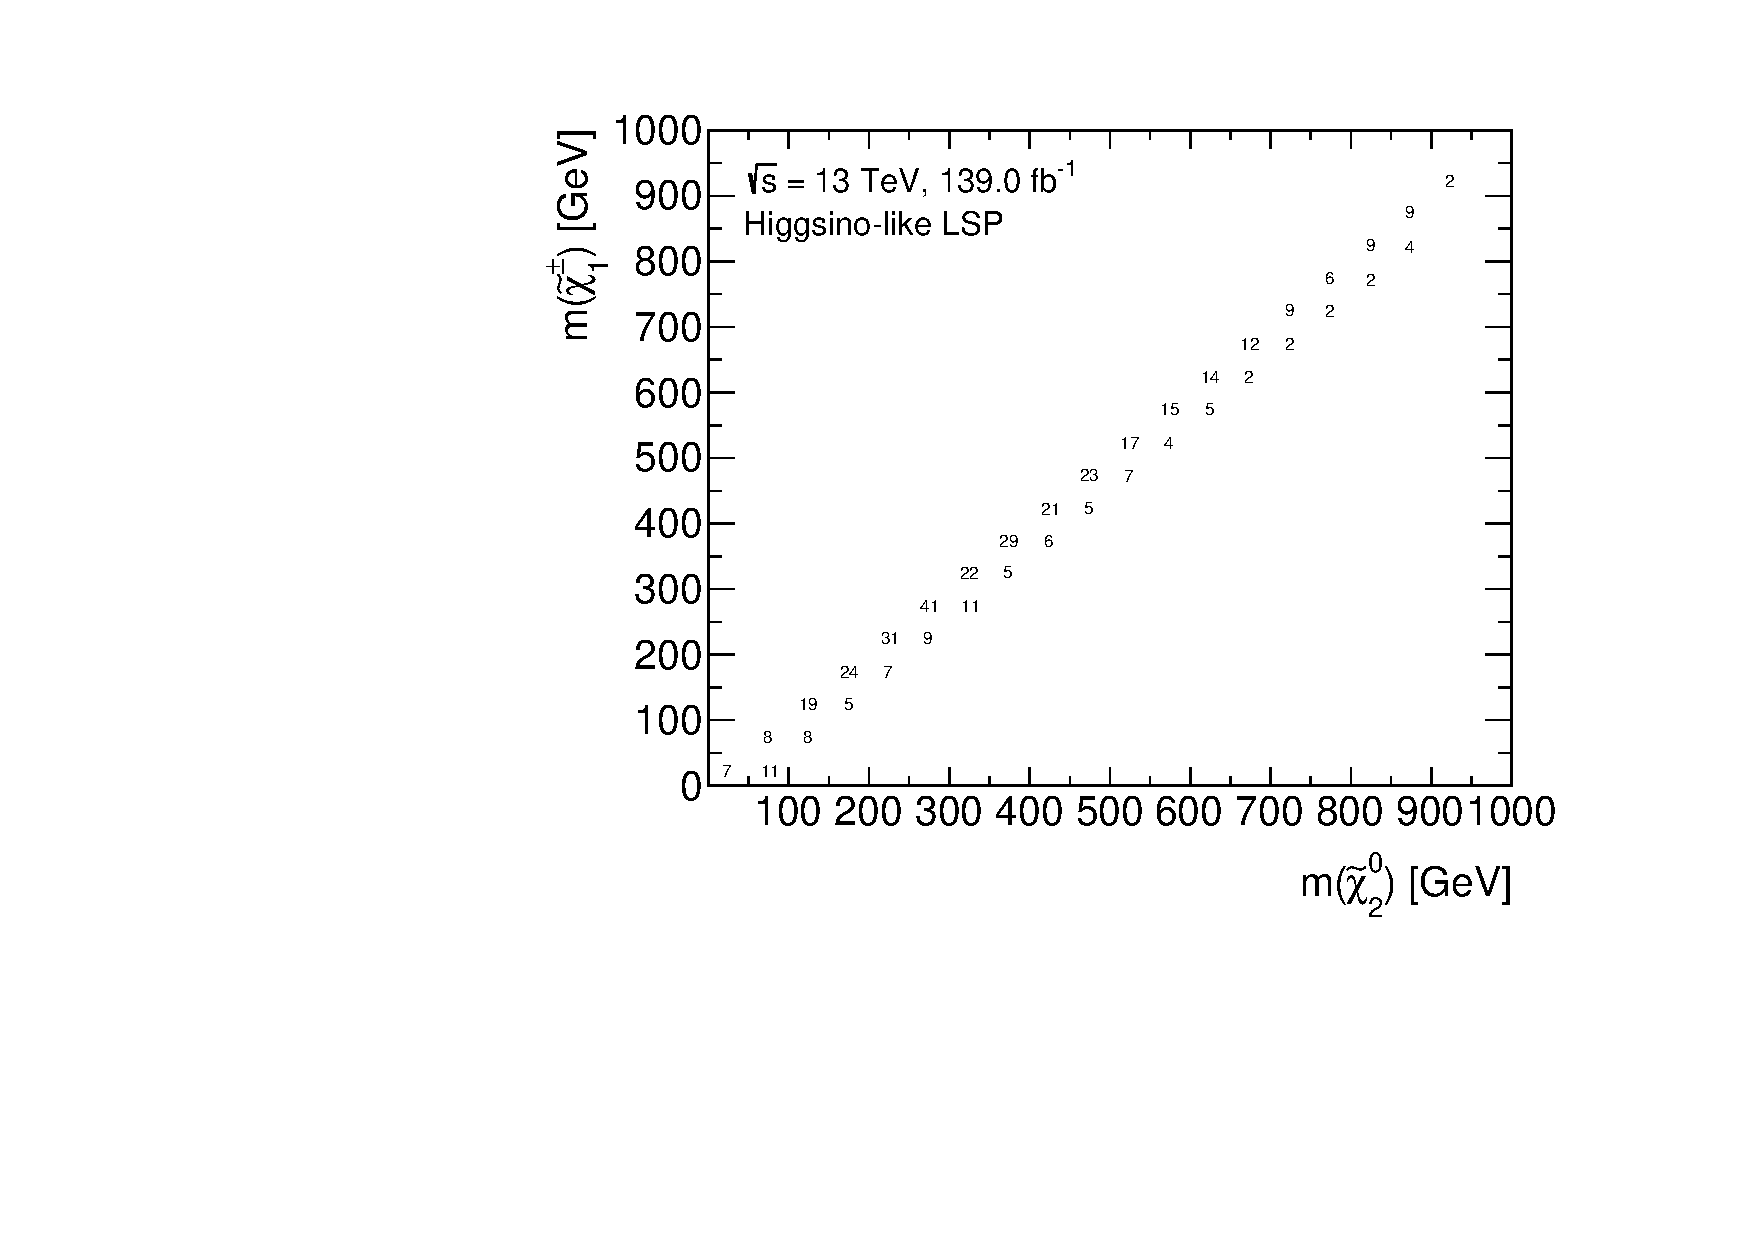
\includegraphics[width=\textwidth]{cut_higgsino_LSP/mchi1p_mchi20_contour}
		\caption{\label{fig:mchi1p_mchi20_contour_higgsino_lsp}}
	\end{subfigure}\hfill
	\caption{Bin-by-bin fraction of excluded models as a function of the relevant sparticle masses. Only \gls{pmssm} models with a higgsino-like \gls{lsp} are shown. The numbers in the bins correspond to the total number of models sampled falling into the respective bin. The number of models excluded by the 1-lepton analysis is encoded with a colour bar ranging from 0 to 1. Where all models in a given bin are excluded, the bin is coloured in black. Bins without a models excluded are left white. Models are evaluated using the simplified likelihood of the 1-lepton analysis. The simplified model contour is shown in orange.}
	\label{fig:impact_electroweakinos_2D_higgsino_lsp}
\end{figure}


\section{Higgs coupling to neutralinos}

\begin{figure}
	\centering
	\begin{subfigure}[b]{0.49\linewidth}
		\centering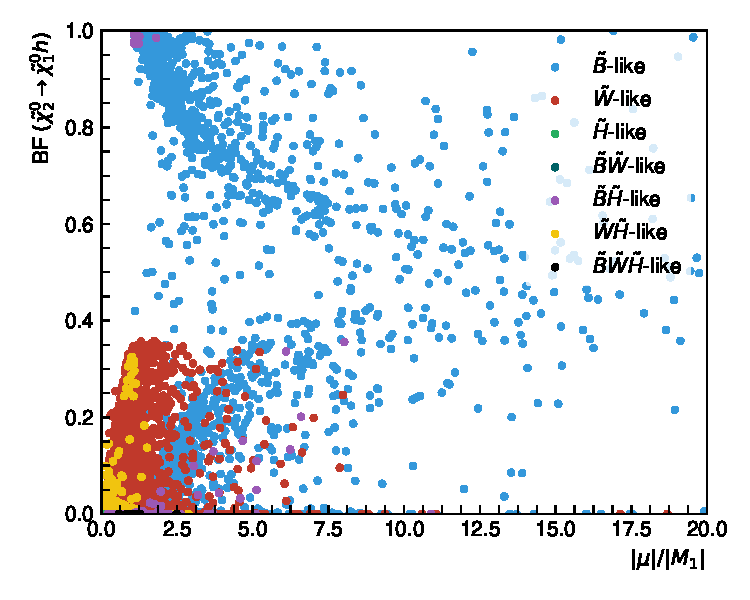
\includegraphics[width=\textwidth]{scatter/lsp_types_BR_Higgs_muM1}
		\caption{\label{fig:lsp_types_BR_Higgs_muM1}}
	\end{subfigure}\hfill
	\begin{subfigure}[b]{0.49\linewidth}
		\centering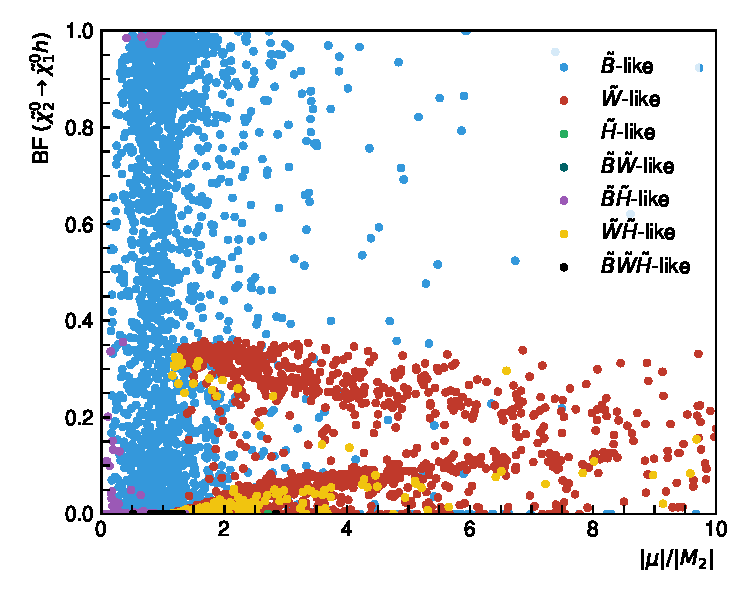
\includegraphics[width=\textwidth]{scatter/lsp_types_BR_Higgs_muM2}
		\caption{\label{fig:lsp_types_BR_Higgs_muM2}}
	\end{subfigure}\hfill
	\caption{}
	\label{fig:higgs_coupling_neutralino}
\end{figure}

\section{Impact of mixed branching fractions}


\begin{figure}
	\centering
	\begin{subfigure}[b]{0.49\linewidth}
		\centering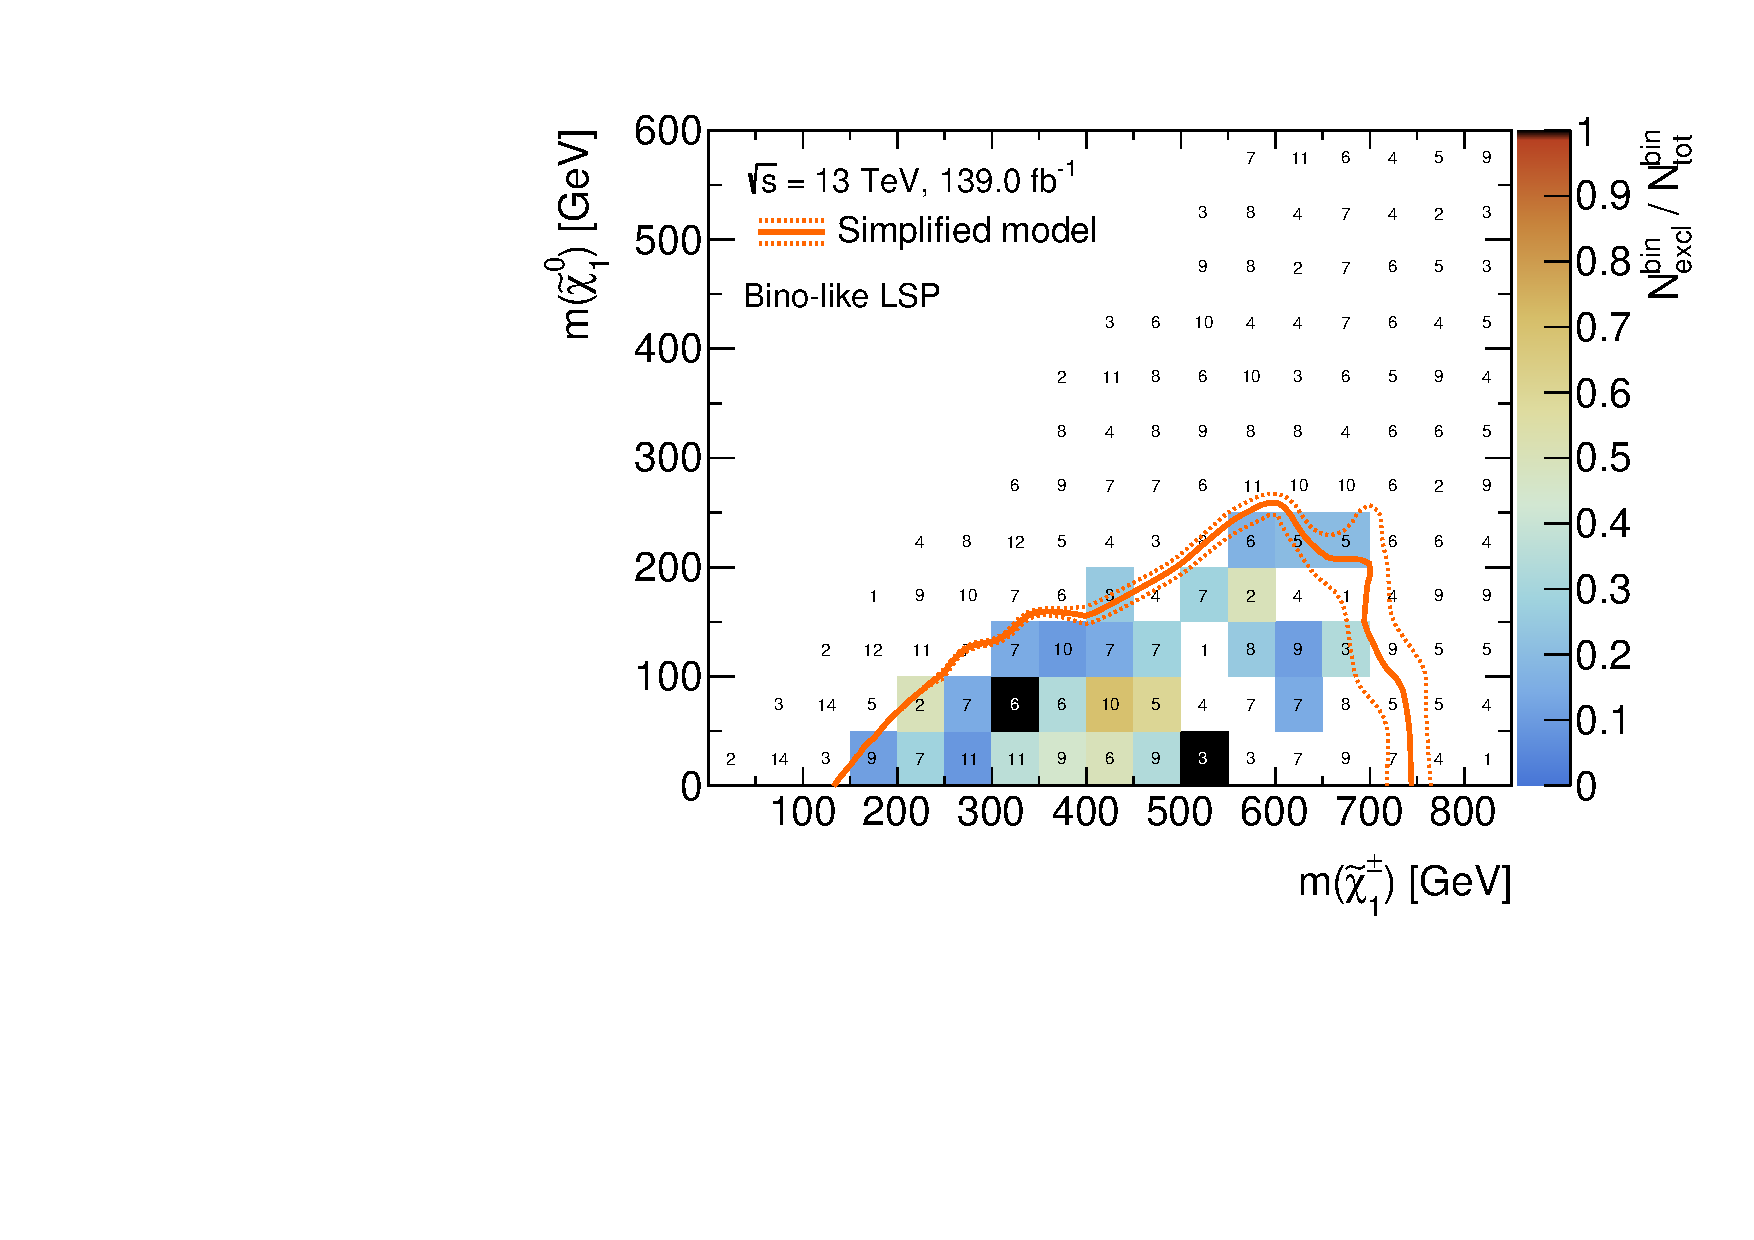
\includegraphics[width=\textwidth]{cut_bino_LSP/mchi1p_mlsp_contour}
		\caption{\label{fig:mchi1p_mchi20_contour_bino_lsp}}
	\end{subfigure}\hfill
	\begin{subfigure}[b]{0.49\linewidth}
		\centering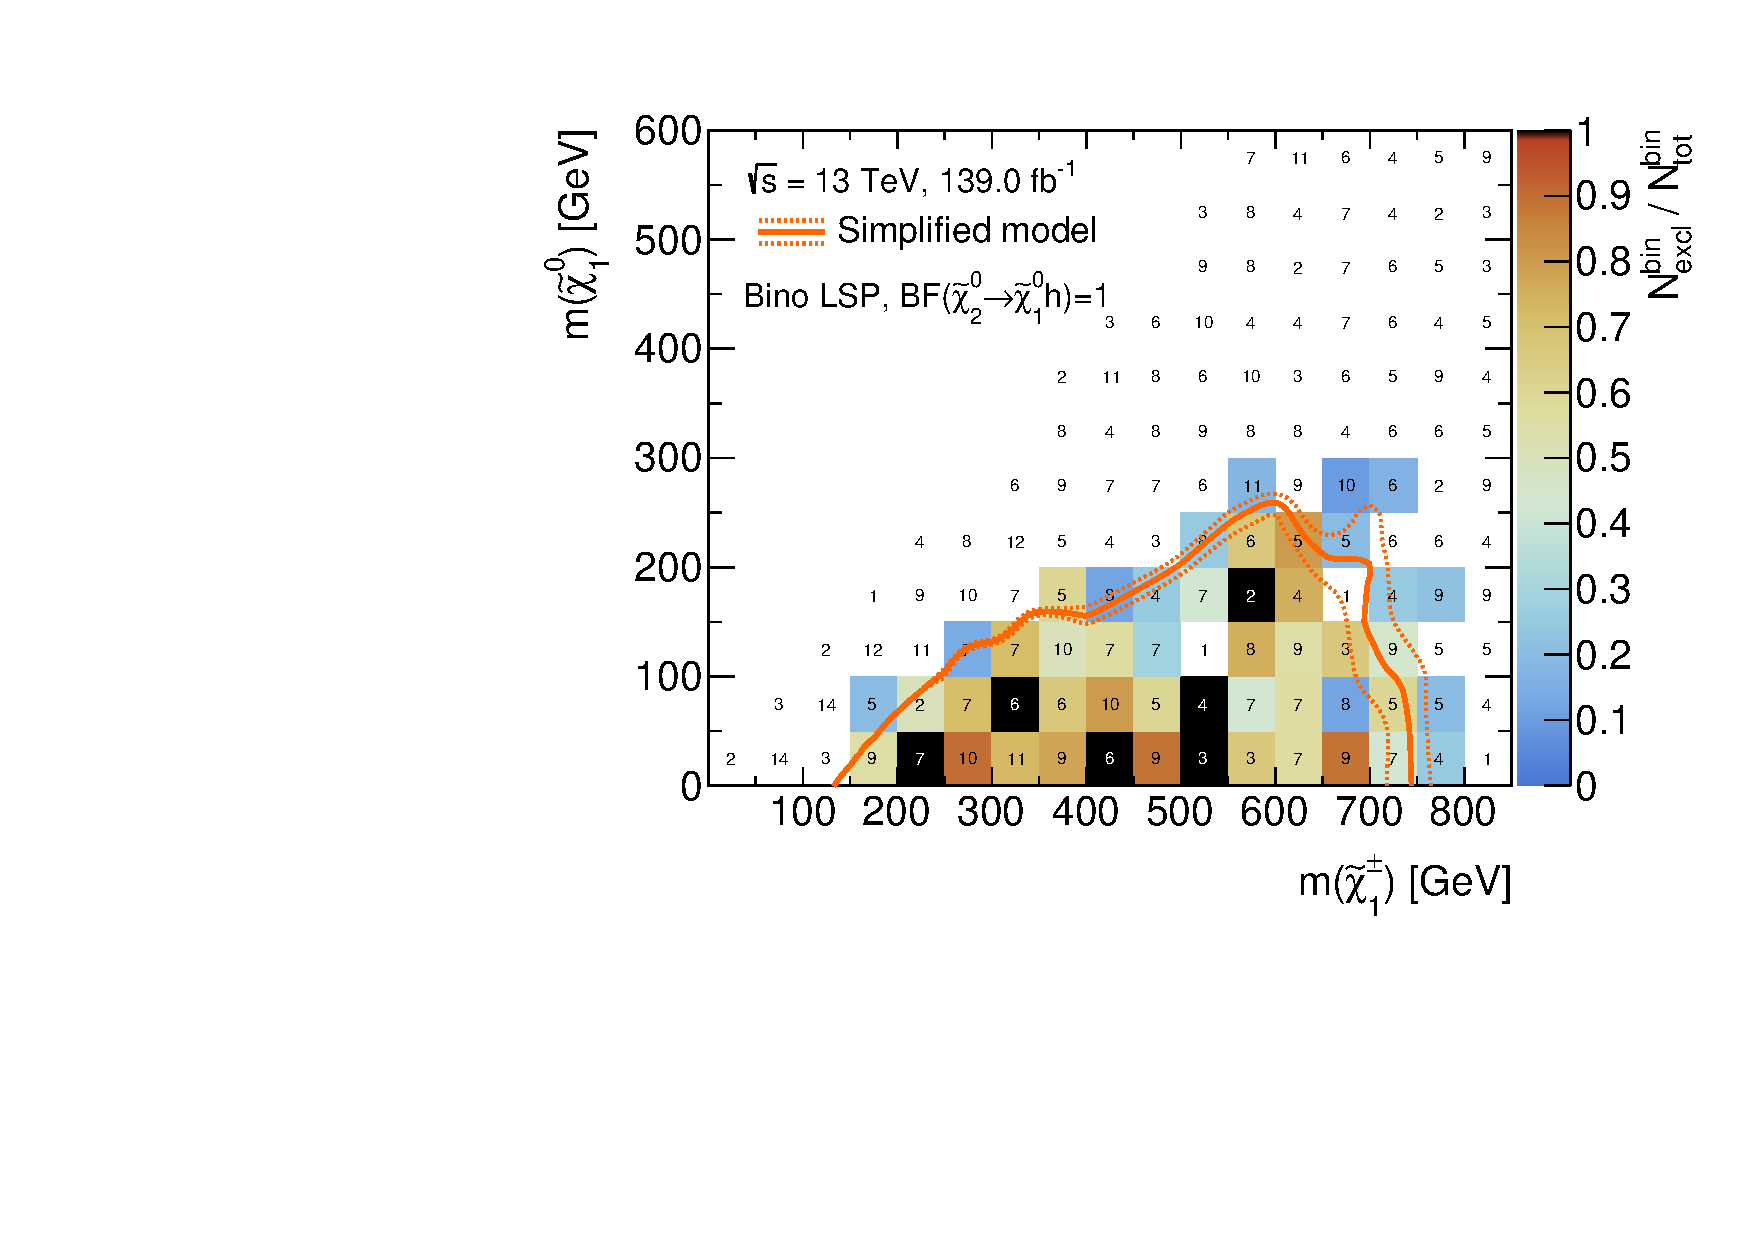
\includegraphics[width=\textwidth]{cut_none_bino_LSP_Wh-only/mchi1p_mlsp_contour}
		\caption{\label{fig:mchi1p_mchi20_contour_bino_lsp_wh_only}}
	\end{subfigure}\hfill
	\caption{}
	\label{fig:mixed_BFs}
\end{figure}

\section{Impact on pMSSM parameters}

\begin{figure}
	\centering
	\begin{subfigure}[b]{0.4\linewidth}
		\centering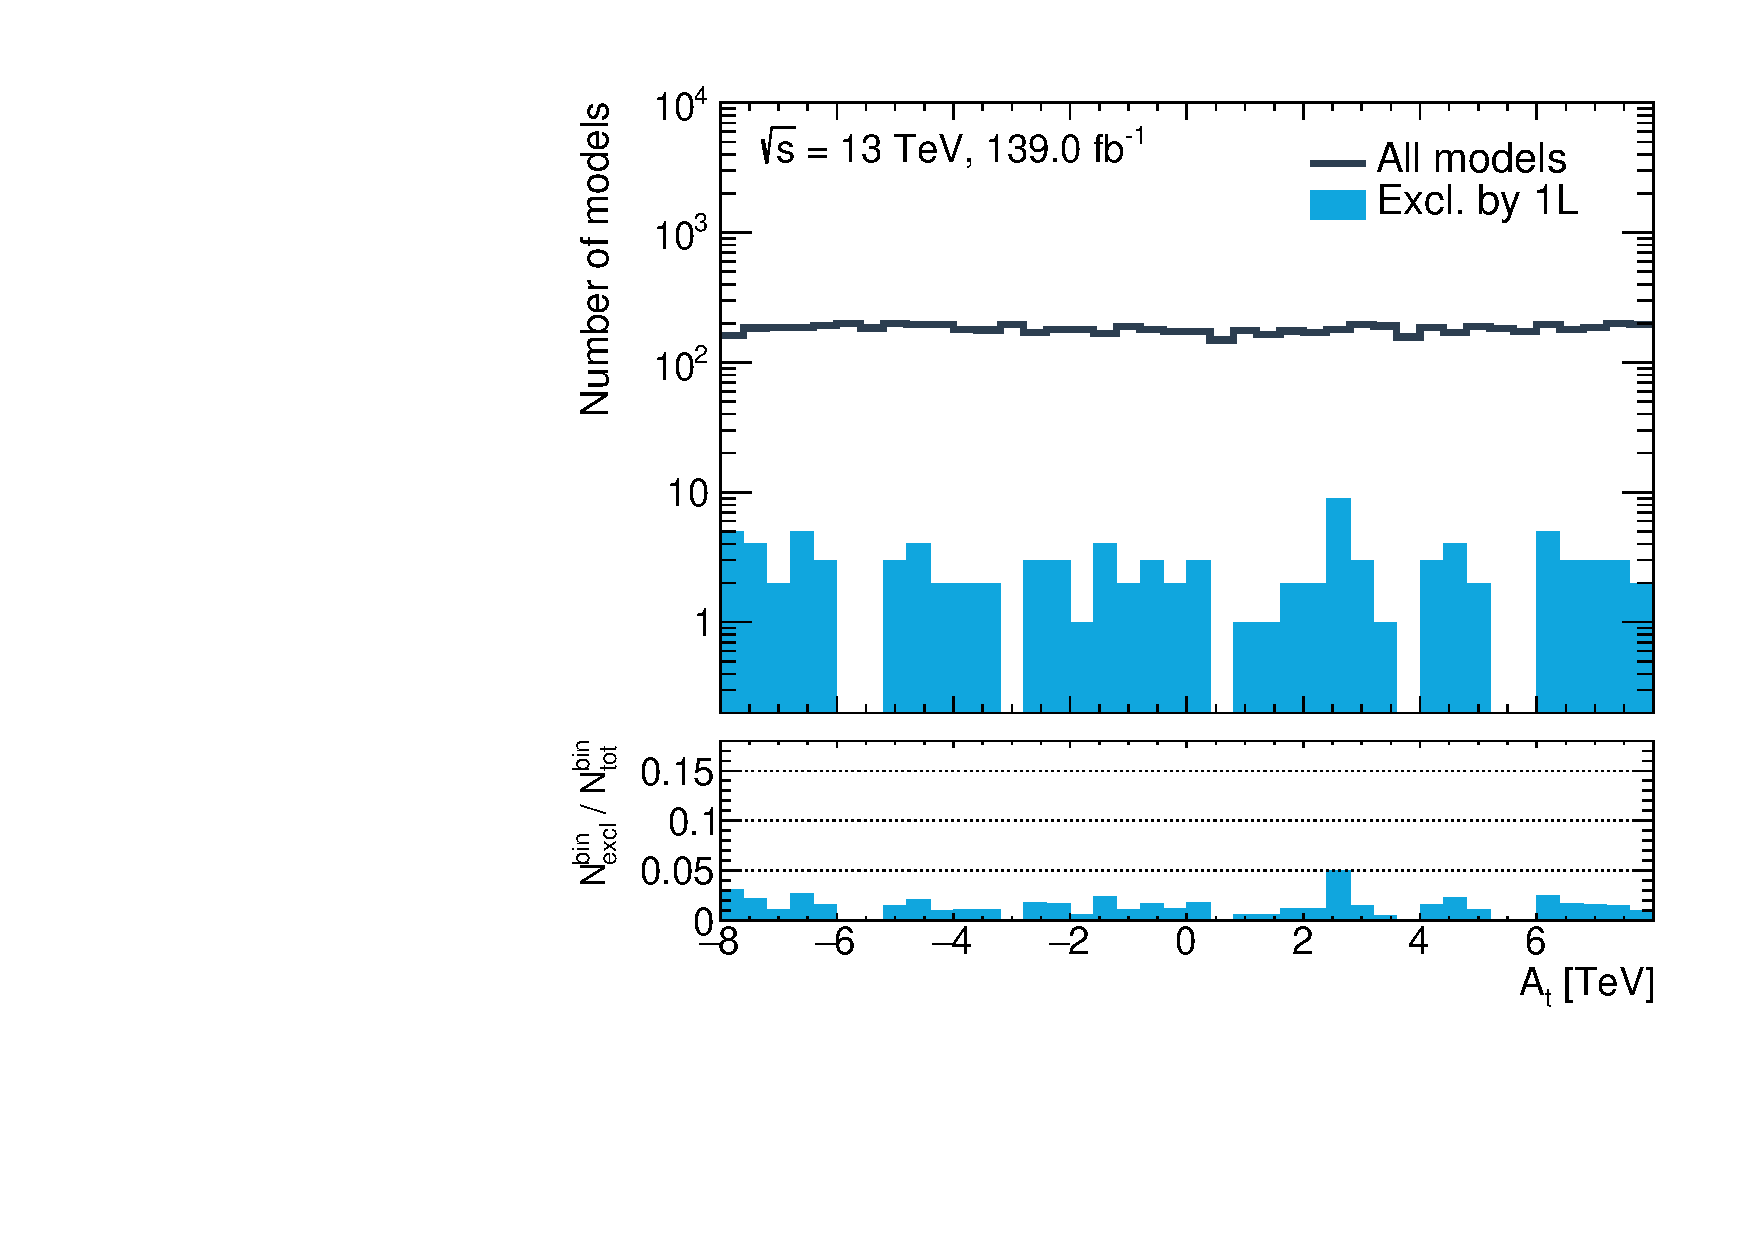
\includegraphics[width=\textwidth]{1D/At}
	\end{subfigure}
	\begin{subfigure}[b]{0.4\linewidth}
		\centering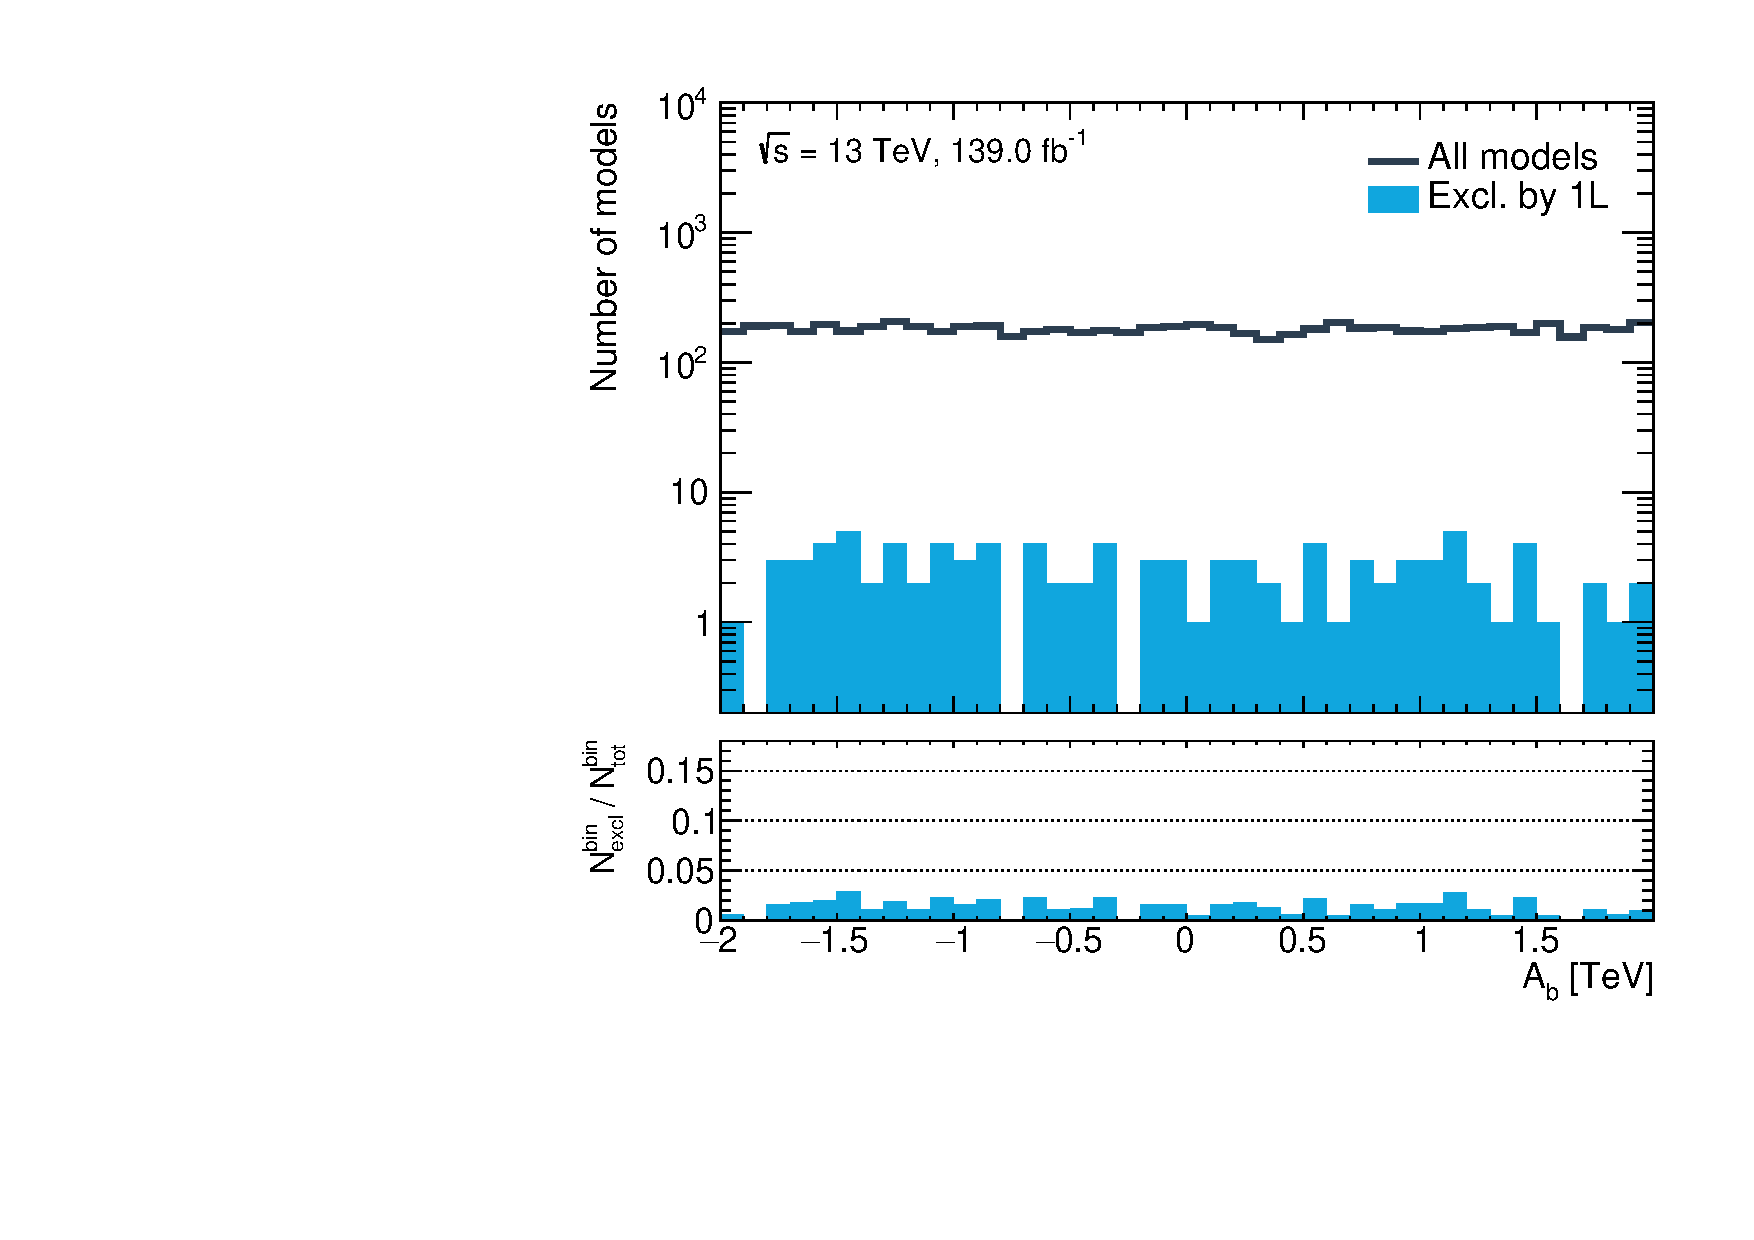
\includegraphics[width=\textwidth]{1D/Ab}
	\end{subfigure}
	\begin{subfigure}[b]{0.4\linewidth}
		\centering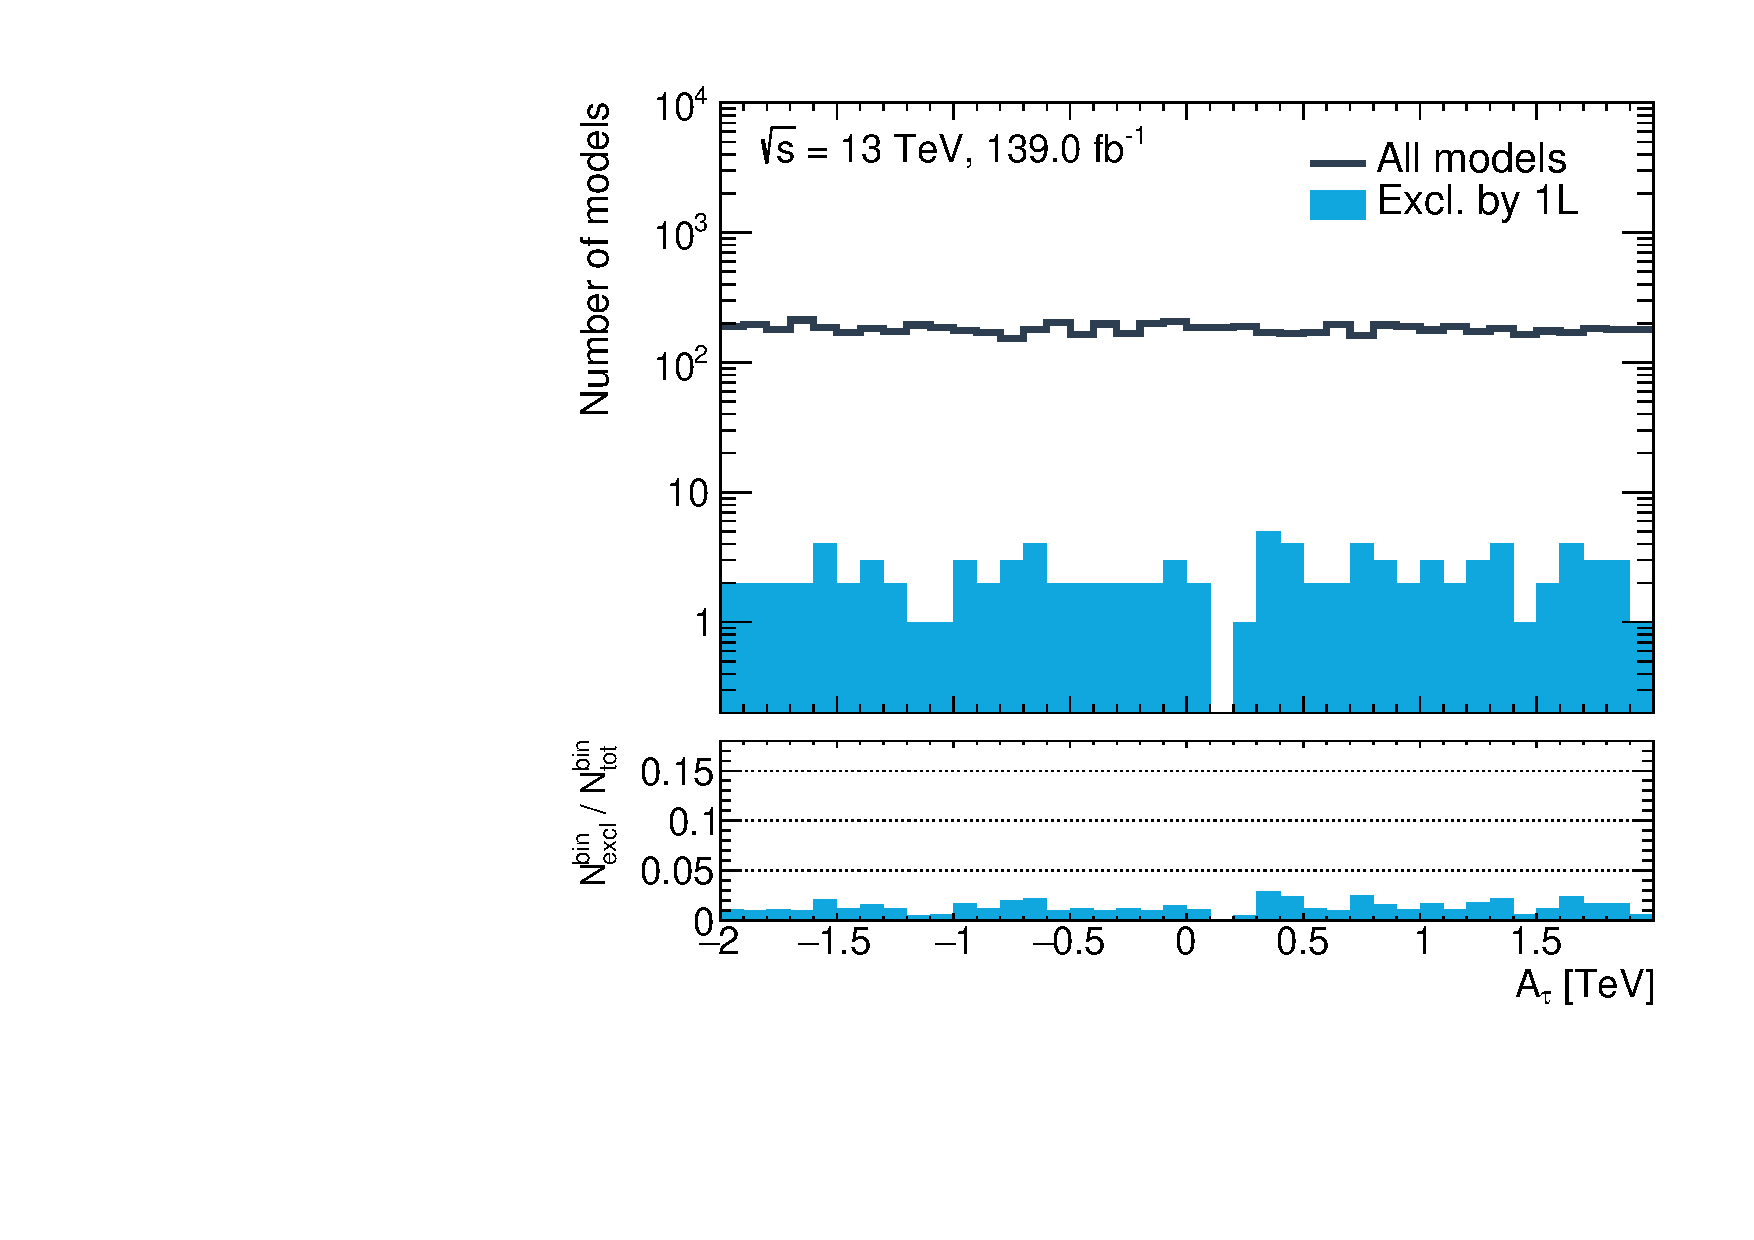
\includegraphics[width=\textwidth]{1D/Atau}
	\end{subfigure}
	\begin{subfigure}[b]{0.4\linewidth}
		\centering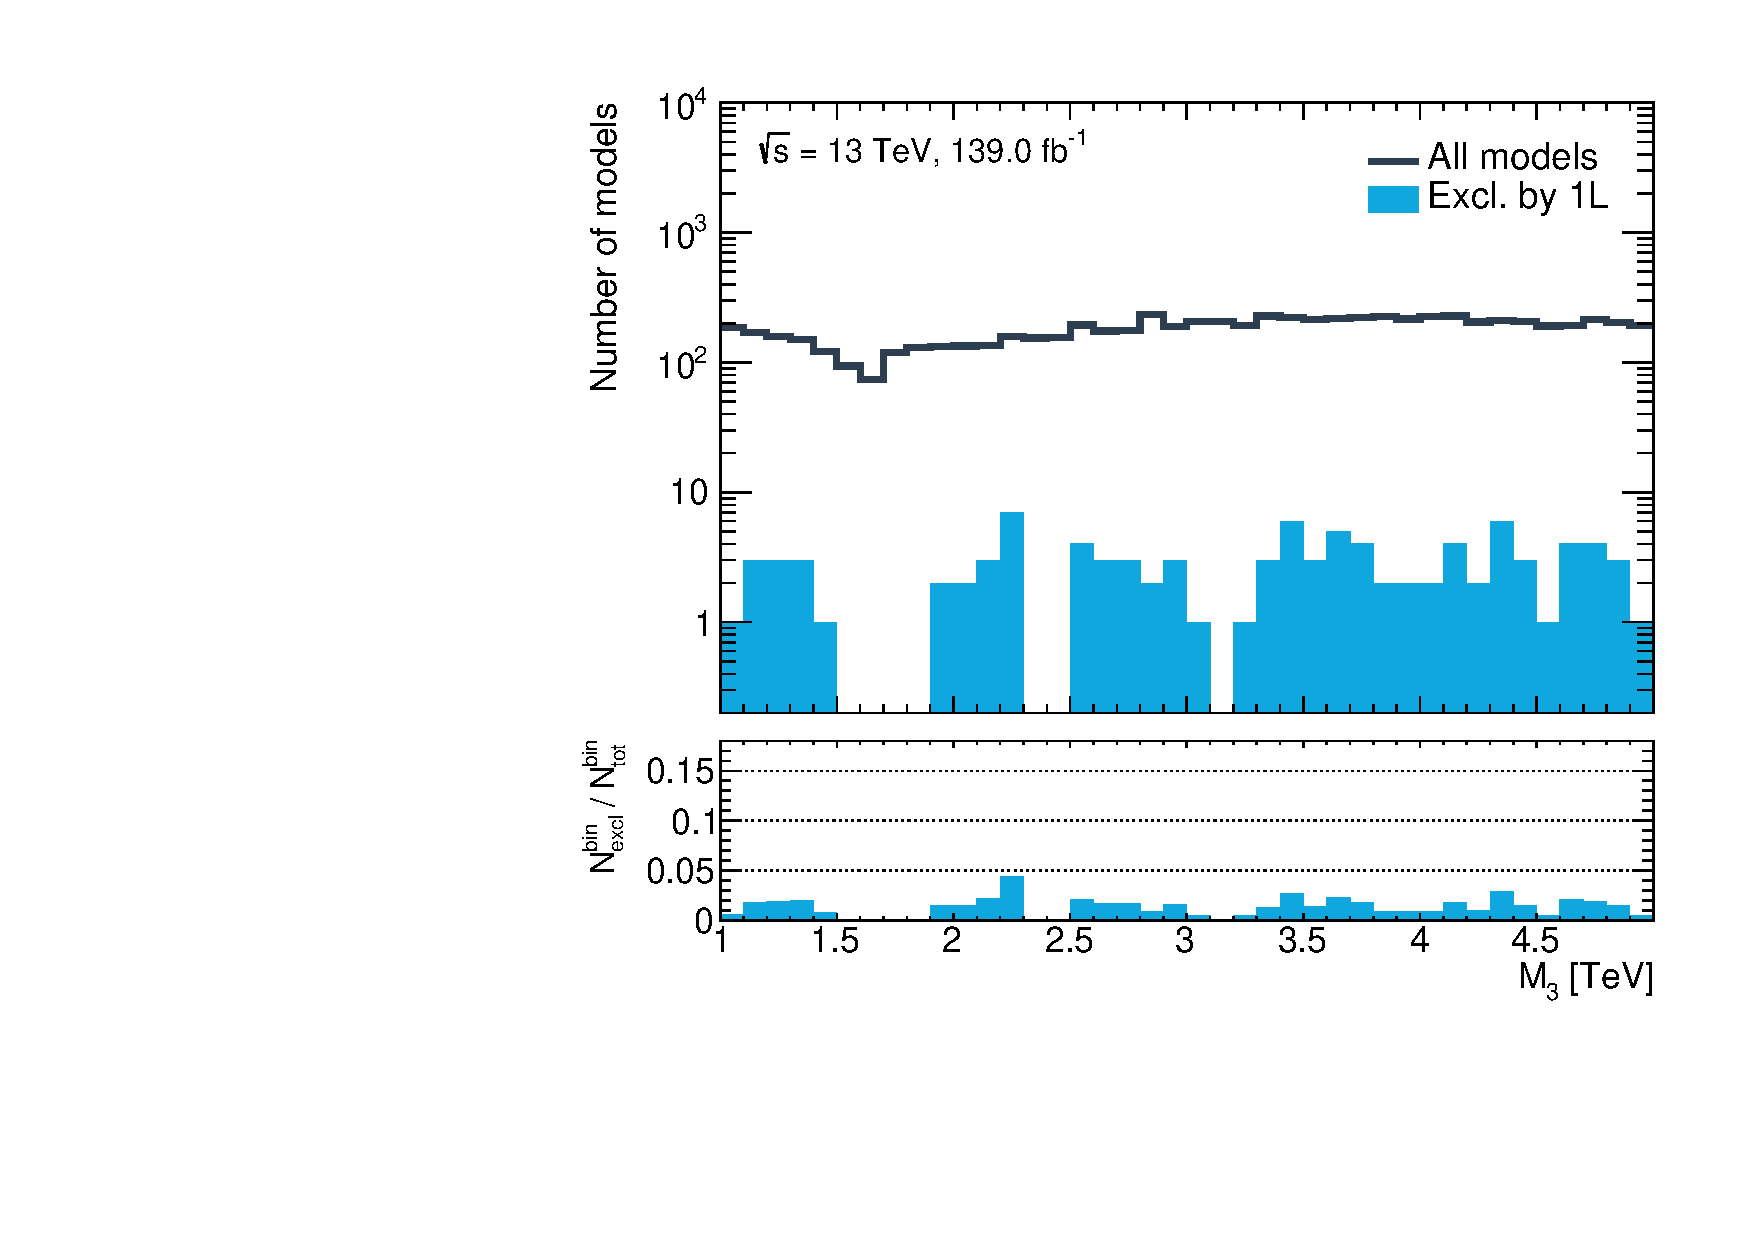
\includegraphics[width=\textwidth]{1D/M3}
	\end{subfigure}
	\begin{subfigure}[b]{0.4\linewidth}
		\centering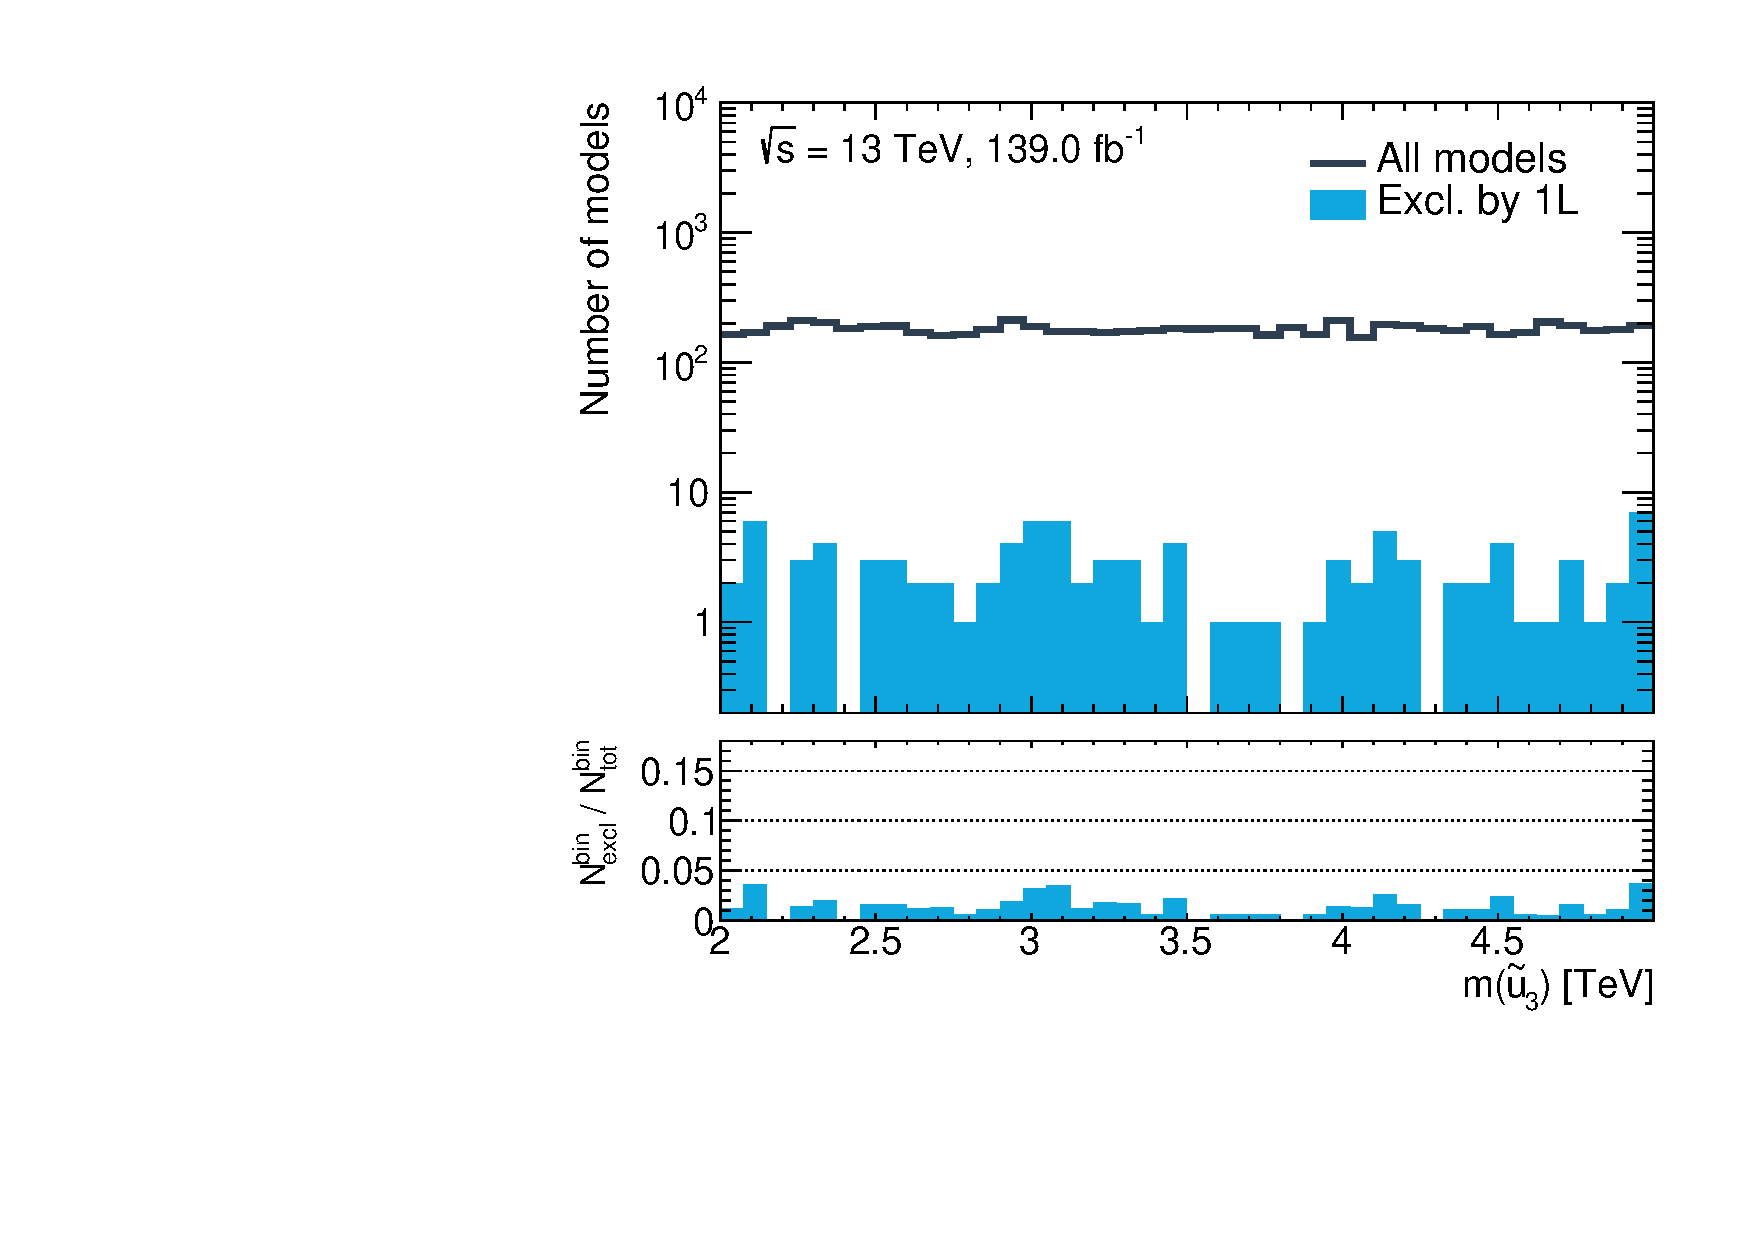
\includegraphics[width=\textwidth]{1D/mtR}
	\end{subfigure}
	\begin{subfigure}[b]{0.4\linewidth}
		\centering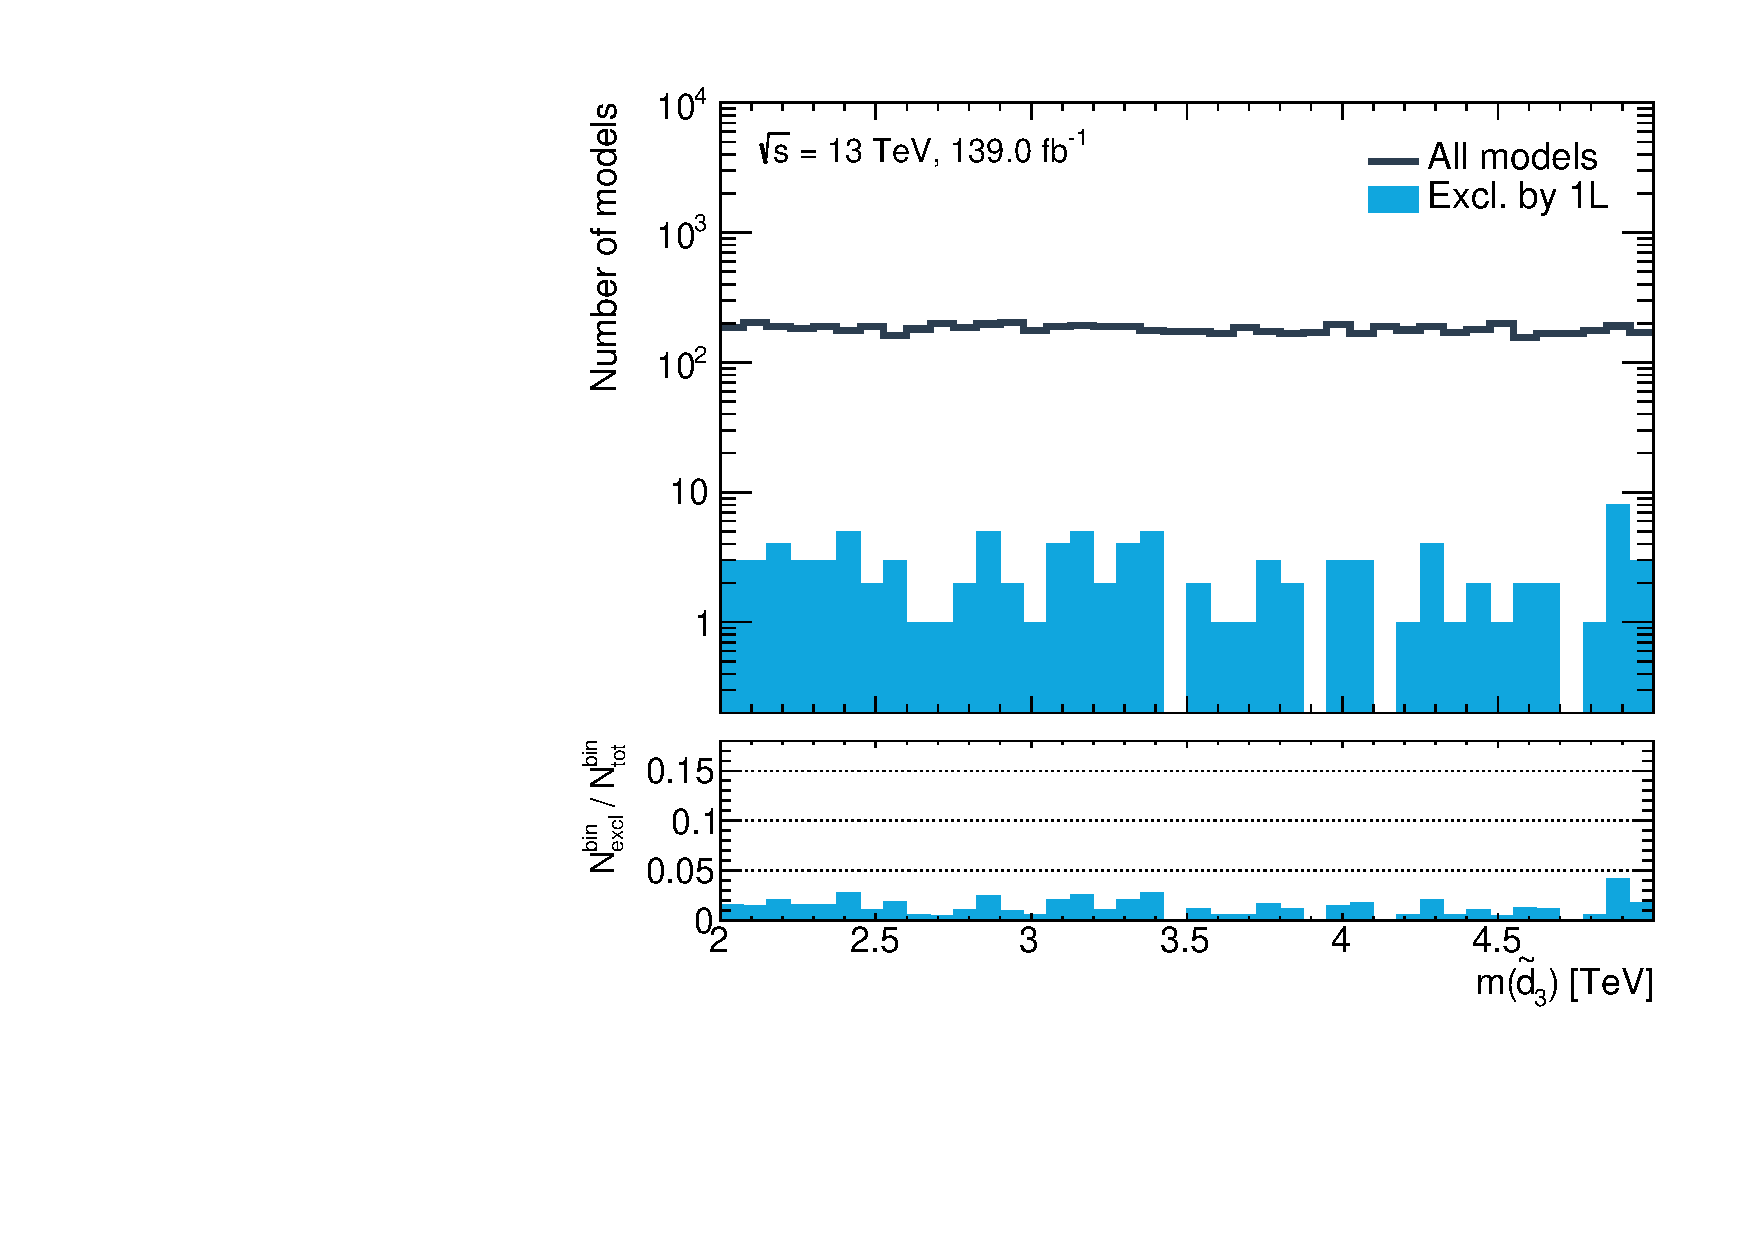
\includegraphics[width=\textwidth]{1D/mbR}
	\end{subfigure}
	\begin{subfigure}[b]{0.4\linewidth}
		\centering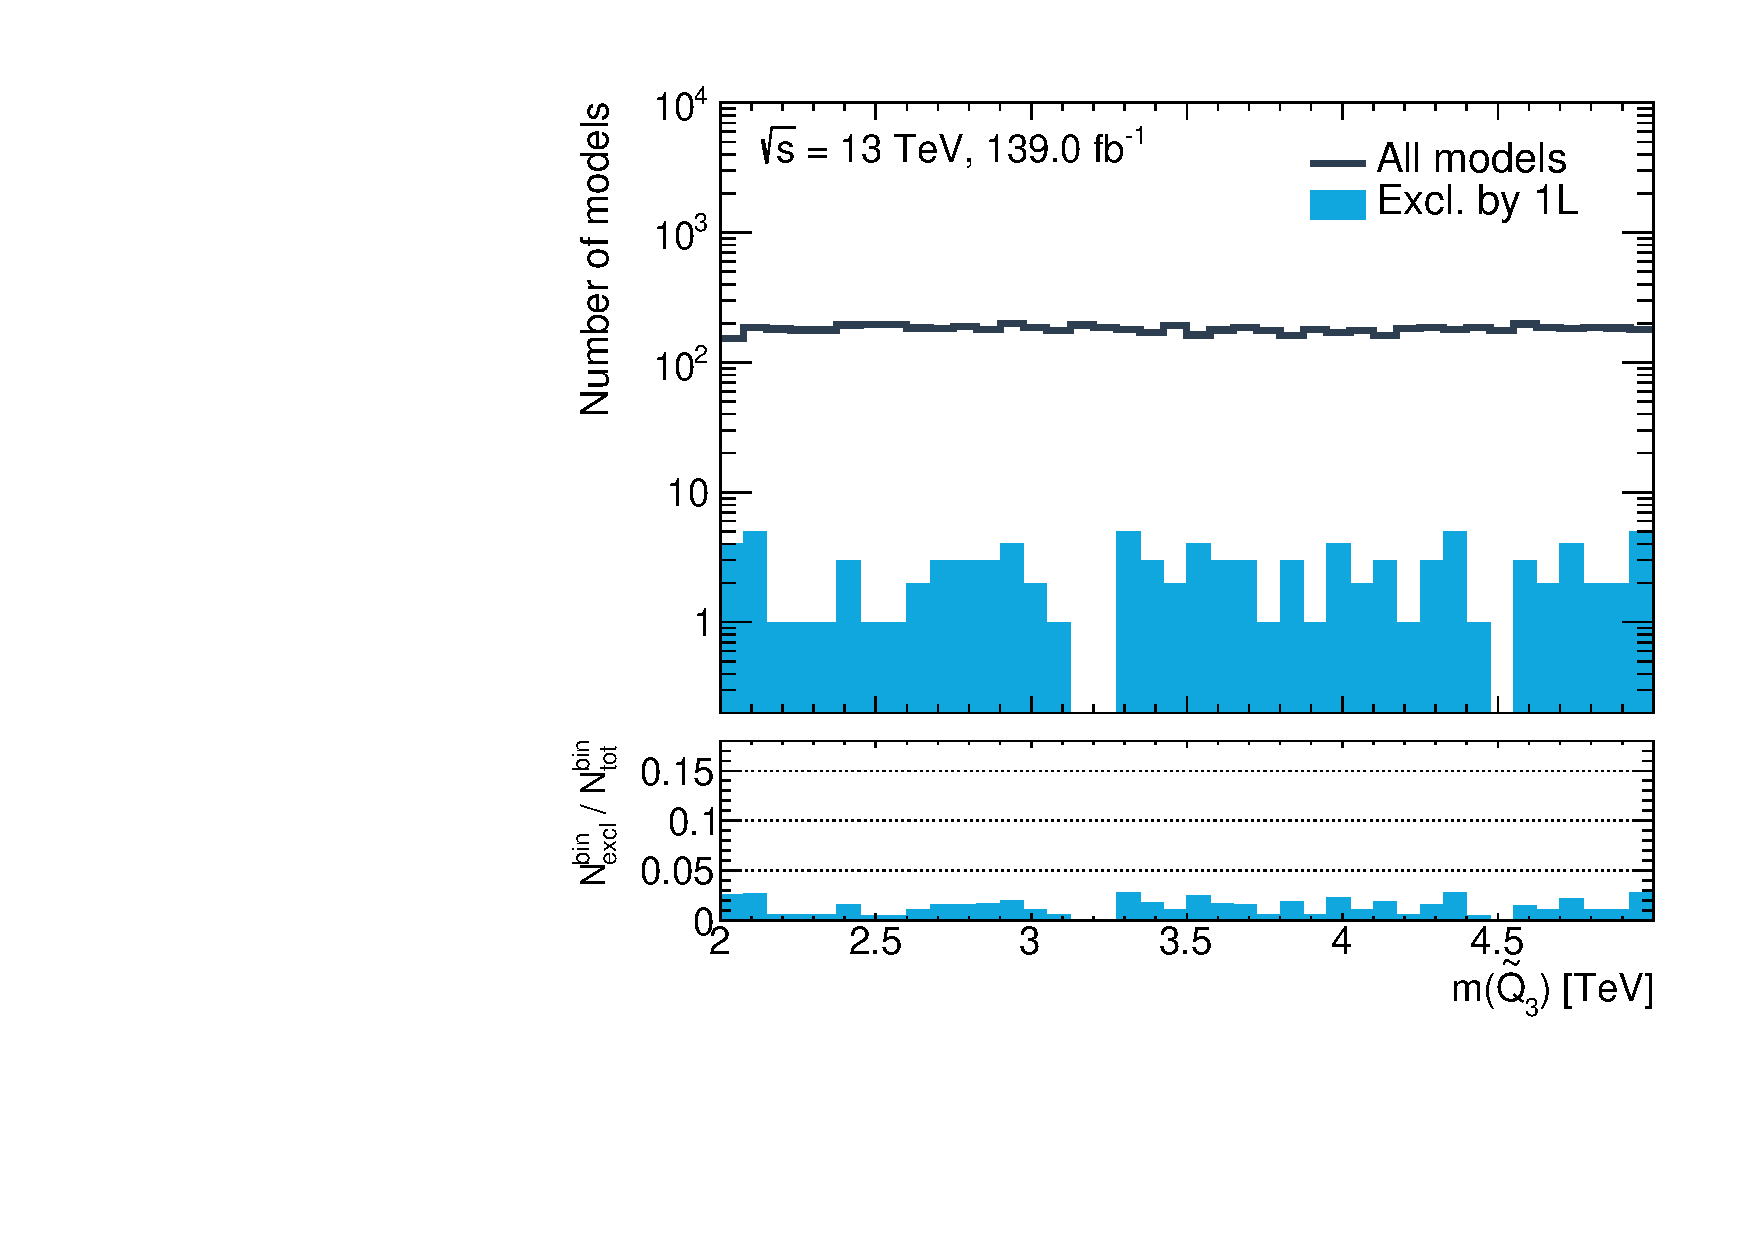
\includegraphics[width=\textwidth]{1D/mqL3}
	\end{subfigure}
	\caption{}
	\label{fig:impact_pMSSM_parameters_1D_2}
\end{figure}

\section{Impact on dark matter relic density}


\begin{figure}
	\centering
	\begin{subfigure}[b]{0.49\linewidth}
		\centering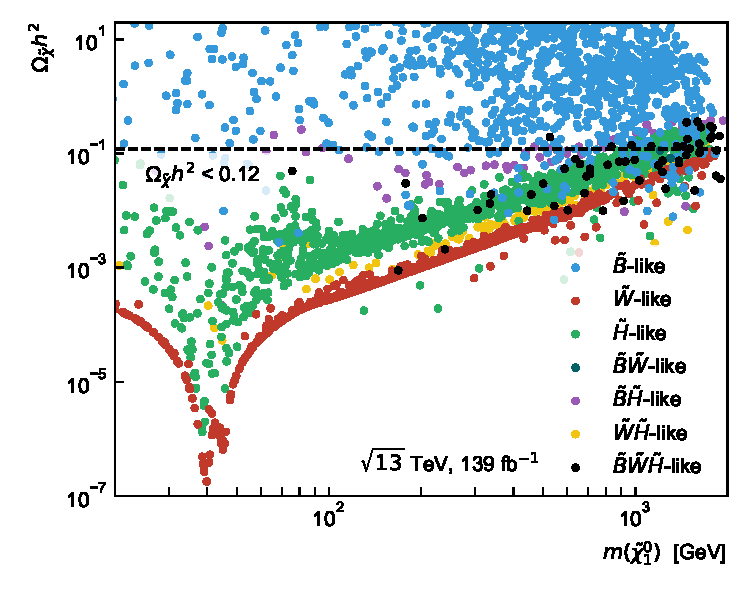
\includegraphics[width=\textwidth]{scatter/relic_density_lsp}
		\caption{\label{fig:relic_density_lsp}}
	\end{subfigure}\hfill
	\begin{subfigure}[b]{0.49\linewidth}
		\centering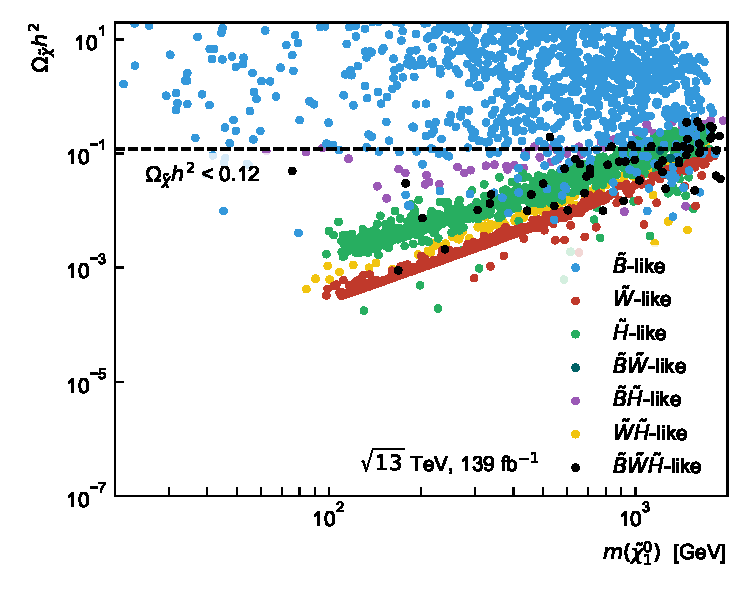
\includegraphics[width=\textwidth]{scatter/relic_density_lsp_constraint}
		\caption{\label{fig:relic_density_lsp_constraint}}
	\end{subfigure}\hfill
	\caption{}
	\label{fig:relic_density_lsp_withConstraint}
\end{figure}
